\chapter{$bbZZ$ Physics Analysis}

In this chapter, we report on a search for the resonant production of a double Higgs boson system. We select Higgs boson pairs that subsequently decay through the $bbZZ$ channel. The final state consists of two b jets, two charged leptons, and two neutrinos ($2 b 2 l 2 \nu$ final state). The analyzed data set was collected in 2016 by the CMS experiment in proton-proton collisions at 13 TeV COM energy, and corresponds to 35.9 fb$^{-1}$ of integrated luminosity. 

\section{Physics analysis overview}
\label{sec:an_overview}

We search for di-Higgs production through the gluon fusion mechanism mediated by two types of possible heavy resonances (separately): a spin-2 Randall-Sundrum (RS1) Kaluza-Klein (KK) graviton and a spin-0 RS1 radion \cite{WED, Xanda}. The width of the graviton and radion is assumed to be negligible with respect to the experimental resolution. We look for decays of WED particles (X) to the $bbZZ$ channel with the two b jets, two charged leptons, and two neutrinos in the final state. However,  the $bbWW$ intermediate channel can also contribute ($0(20)\%$) to the final state of this measurement. Therefore, the full chain of this measurement is $X \rightarrow HH \rightarrow bbZZ/bbWW \rightarrow 2 b 2l 2 \nu$. In the above, one of the Higgs bosons decays to a pair of b quarks and the other Higgs boson decays to ZZ or WW system. For the purposes of this measurement, we consider only leptonic decays of ZZ and WW. Intermediate taus are included when the decay to daughter muons and electrons. We explore the invariant masses of WED particles ranging from 250 to 1000 GeV. The result of the measurement is the upper limit on the production cross section of the resonance multiplied by the branching fraction of its decay into the aforementioned $2 b 2 l 2 \nu$ final state. 

In this data analysis (later referred to as the ``analysis''), we will describe first the data sets (often referred to as ``datasets'') and data triggers. The measurement uses the DoubleEG and DoubleMuon PDs defined in the previous chapter. These di-electron and di-muon channels are analyzed separately and the information is combined in the final result. To select the events with two prompt charged leptons, a set of triggers was applied, when the events were recorded. To increase the statistics of the measurement and maximize the number of leptons passing the selection, certain complex trigger strategies were employed. 

We then discuss the MC simulation of the signal and background processes (later referred to as ``signal'' and ``background''). The signal MC samples had to be produced for both graviton and radion particles for 16 mass points from 250 to 1000 GeV to cover the whole search range. 

The description of the physics object reconstruction and event selection was given in the previous chapter. Physics objects are constructed using the information from the CMS subsystems and the output of the PF algorithm. Then, based on the final state signature, the events containing corresponding physics objects are selected. The construction of the Higgs and Z boson candidates is discussed at length. The characteristics of the signal and background processes are specified and data-MC SFs are discussed.

A signal and background control regions are defined in the kinematic space of the candidates. The MVA technique is used to improve signal-background discrimination. We rely on the BDT classifier (commonly referred to as the BDT for brevity) to reduce the contribution of background processes in the signal region. In all physics measurements, there are sources of systematic and statistical uncertainties that affect the final results. We discuss all major uncertainties at length and specify the size of the effect of individual types of uncertainties on the final result. 

We present the statistical analysis used to extract the results of the measurements and discuss the CMS statistical package that has been used to extract the final results. Then, we present the results of the measurement and compare them with the theoretical predictions. Finally, we discuss the ``grand $HH$ combination'' using measurements of all available $HH$ channels.

The material in this chapter follows the description of two articles to which the author contributed directly \cite{bbZZAN, CMS-PAS-HIG-17-032}.

\section{Data analysis strategy}
\label{sec:strategy}
We form the Lorentz energy-momentum vector associated with the double Higgs system. This vector is constructed as the sum of the Lorentz vectors of the two leptons, two b jets, and the four-vector representing neutrinos ($\vec{p}^{miss}_T$). As the z component of the neutrinos' momentum is unknown, we form a pseudo-transverse mass:
$\tilde{M}_T(HH) = \sqrt{E^2 - p_{z}^2}$ (further referred to as the ``transverse mass'' for brevity), where $E$ and $p_z$ are the energy and the z-axis component of the Lorentz energy-momentum vector of the di-Higgs candidate. Because $p_z$ of the neutrinos is unknown and varies from event to event, the variable \mTHH has a distribution, the shape of which depends on the mass of the intermediate resonance and how much energy is carried by the neutrinos.

\mTHH distributions are derived for 16 masses and for both spin hypotheses. The \mTHH is constructed using signal and background simulations. The distributions are produced separately for the signal-enriched (SR) and control regions (CR), which are defined later in this chapter.

To extract the final results, we perform a simultaneous fit of the sum of the signal and background \mTHH distributions in the SR and CRs to the data. The fits are produced for both di-electron and di-muon channels and the results are combined. We obtain 95\% CL upper limits on the $HH$ production cross section multiplied by the BFs of the subsequent decay to the final state of this measurement. The employed statistical method is based on the CL$_{S}$ asymptotic procedure~\cite{Zech:1988un}.

\section{Data and Triggers}
\label{sec:data_and_triggers}

\subsection{Data}
The search is performed using DoubleMuon and DoubleEG PDs recorded by CMS in 2016.
%corresponding to an integrated luminosity of 35.9 fb$^{-1}$ recorded by the CMS experiment during Run 2 in 2016. 
%The data were produced in proton-proton collisions at the LHC at 13 TeV COM energy. 
The data were collected in several data taking periods and approximate values of the integrated luminosity of these periods are given in Table \ref{tab:datasets}.

\begin{table}[htbp]
\caption[List of data sets collected by the CMS in 2016.]{List of data sets collected by the CMS in 2016. Each era contains a unique letter identifier. Also, the date of the data processing is specified. If re-processing was run, it is labeled as ``v2''. Corresponding integrated luminosities are shown in the second column.
}
\label{tab:datasets}
\begin{center}
\scalebox{0.8}{
\begin{tabular}{|c|c|} \hline%\hline
Dataset & $\int\mathcal L$ dt (\fbinv) \\
\hline
%{\texttt Run2016B-03Feb2017-v1} & \multirow{2}{*}{$\sim$5.9} \\
{\texttt Run2016B-03Feb2017-v2} & {$\sim$5.9} \\
%{\texttt Run2016B-03Feb2017-v2} & \\
{\texttt Run2016C-03Feb2017-v1} & $\sim$2.7 \\
{\texttt Run2016D-03Feb2017-v1} & $\sim$4.3 \\
{\texttt Run2016E-03Feb2017-v1} & $\sim$4.1 \\
{\texttt Run2016F-03Feb2017-v1} & $\sim$3.2 \\
{\texttt Run2016G-03Feb2017-v1} & $\sim$3.8 \\
{\texttt Run2016H-03Feb2017-v1} & $\sim$11.8 \\
\hline
Total Luminosity & $\sim$35.9 \\
\hline%\hline
\end{tabular}
}
\end{center}
\end{table}

\subsection{Triggers\label{sec:triggers}}

The data events that are used in this measurement are selected with a set of HLT triggers that required the presence of two muons or two electrons in the event. In the di-electron final state, the trigger requires the leading electron to have $p_T$ above 23 GeV, and the sub-leading electron to have $p_T$ above 12 GeV. In offline selection $p_T$ selection is increased to 25 and 15 GeV correspondingly. %The latter leg corresponds to a relatively low-efficiency electron. Since the measurement is focused on ``golden'' electrons coming from on-shell Z boson decays, the offline selection is slightly tighter than the HLT selection and requires the sub-leading electron to have $p_T$ above 15 GeV.
The final state that contains two prompt muons is selected with an HLT path which is a combination of several HLT paths chained together using the logical ``OR'' operation. In other words, the muons are required to pass the selection of at least one of the HLT paths. At the HLT level, the leading and sub-leading muons have to pass the 17 and 8 GeV $p_T$ requirements respectively. The difference among HLT paths has been explained at length in Section \ref{ch:cms}. The offline analysis increases the $p_T$ threshold values to 20 and 15 GeV correspondingly. For the offline selection, electrons are selected in the range $|\eta| < $ 2.5 and muons in the range $|\eta| < $ 2.4. For both channels, the $|\eta|$ region in the gap (1.4442 to 1.566) between the barrel and endcap is excluded.

The same trigger selections are applied to MC simulated events to mimic the selection in data. The efficiencies are then derived for MC and data, and SFs are determined using the TnP procedure discussed in Section \ref{sec:TnP}. Trigger SFs have been computed for each trigger leg separately since the selection of each leg varies (Fig. ~\ref{fig:trigger_eff_diele}). Following the recommendations from the CMS Muon POG, scale factors have been calculated separately for two data collecting periods: runs B to G (Fig. \ref{fig:trigger_SF_dimu_BCDEFG}, and run H separately (Fig. \ref{fig:trigger_SF_dimu_H}), since the LHC conditions varied significantly for the run H. All eras have slightly different integrated luminosities, see Table \ref{tab:datasets}, so the final SFs are luminosity averaged. Additionally, as was discussed in the chapter on CMS Physics Objects Reconstruction, some triggers did not contain the DZ requirement, while others did. Therefore, scale factors of the DZ selection are also measured, see Fig. \ref{fig:trigger_SF_dimu_dZ_H}). Prior to measuring the trigger scale factors, the electrons and muons were required to satisfy ID and ISO selections; more details are given in the subsections \ref{sec:electrons}, \ref{sec:muons}. 

\begin{figure}[H]
\centering
\subfloat Leg 1
{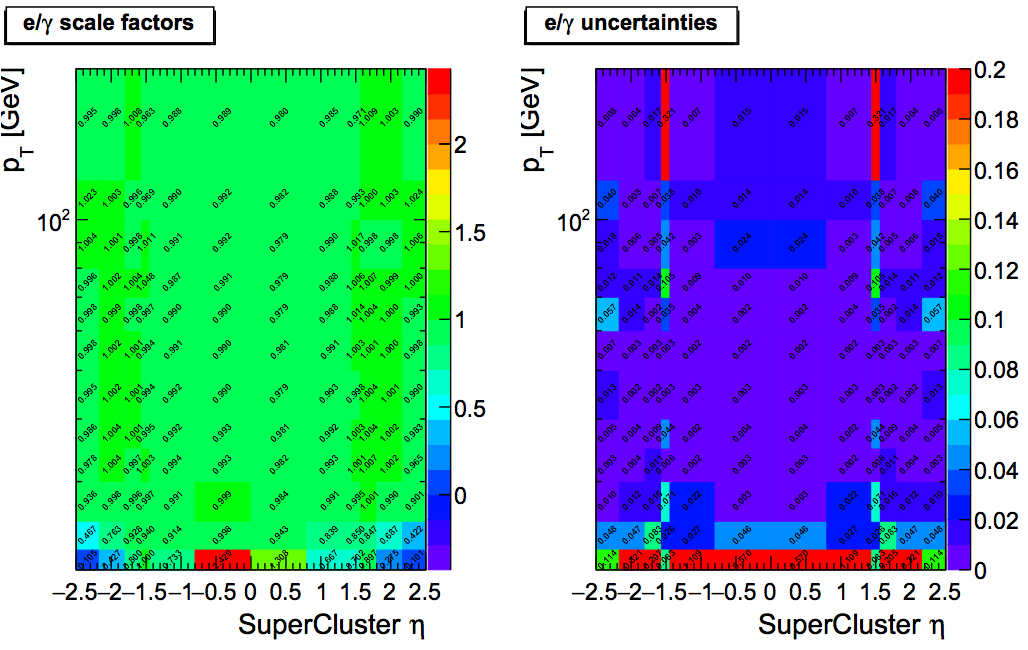
\includegraphics[width=1.0\textwidth]{trigger/electronTriggerEfficiencyelectronTriggerEfficiencyHLT_Leg1_WP90_2016.png} } \\
\subfloat Leg 2
{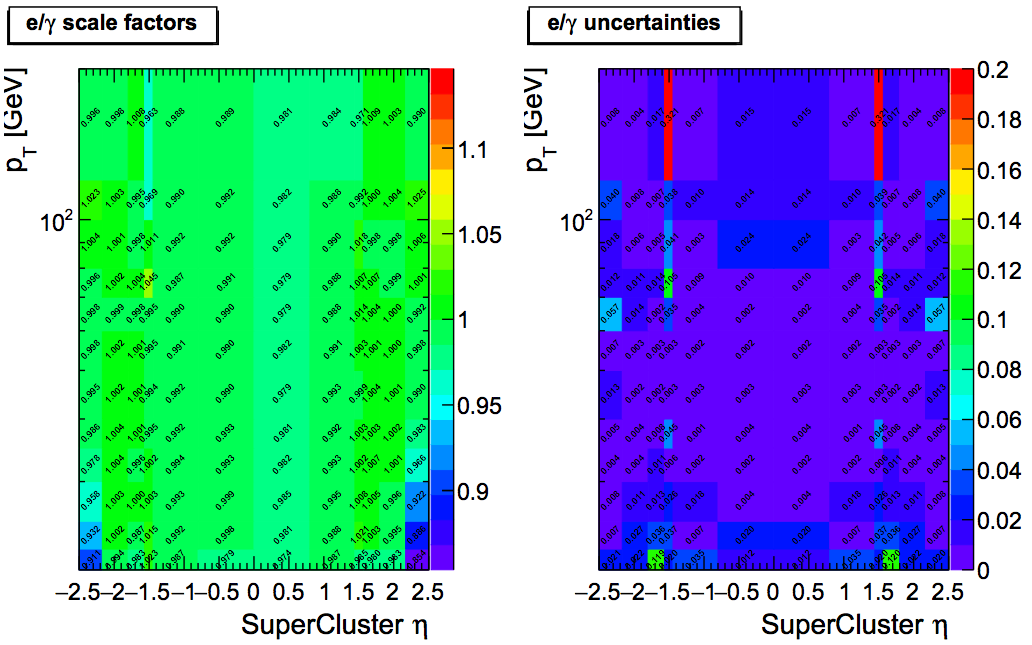
\includegraphics[width=1.0\textwidth]{trigger/electronTriggerEfficiencyelectronTriggerEfficiencyHLT_Leg2_WP90_2016.png} } \\
\caption[HLT trigger SFs for electrons.]{HLT trigger SFs for electrons approved by the CMS $e/ \gamma$ POG group. SFs are derived for both legs separately: Leg 1 (top) corresponds to the leading electron and Leg 2 (bottom) corresponds to the sub-leading electron. The values of the SFs are shown on the left, and the associated uncertainties with each value are shown on the right. Taken from ~\cite{vhbbAN}.}
\label{fig:trigger_eff_diele}
\end{figure}

\begin{figure}[H]
\centering
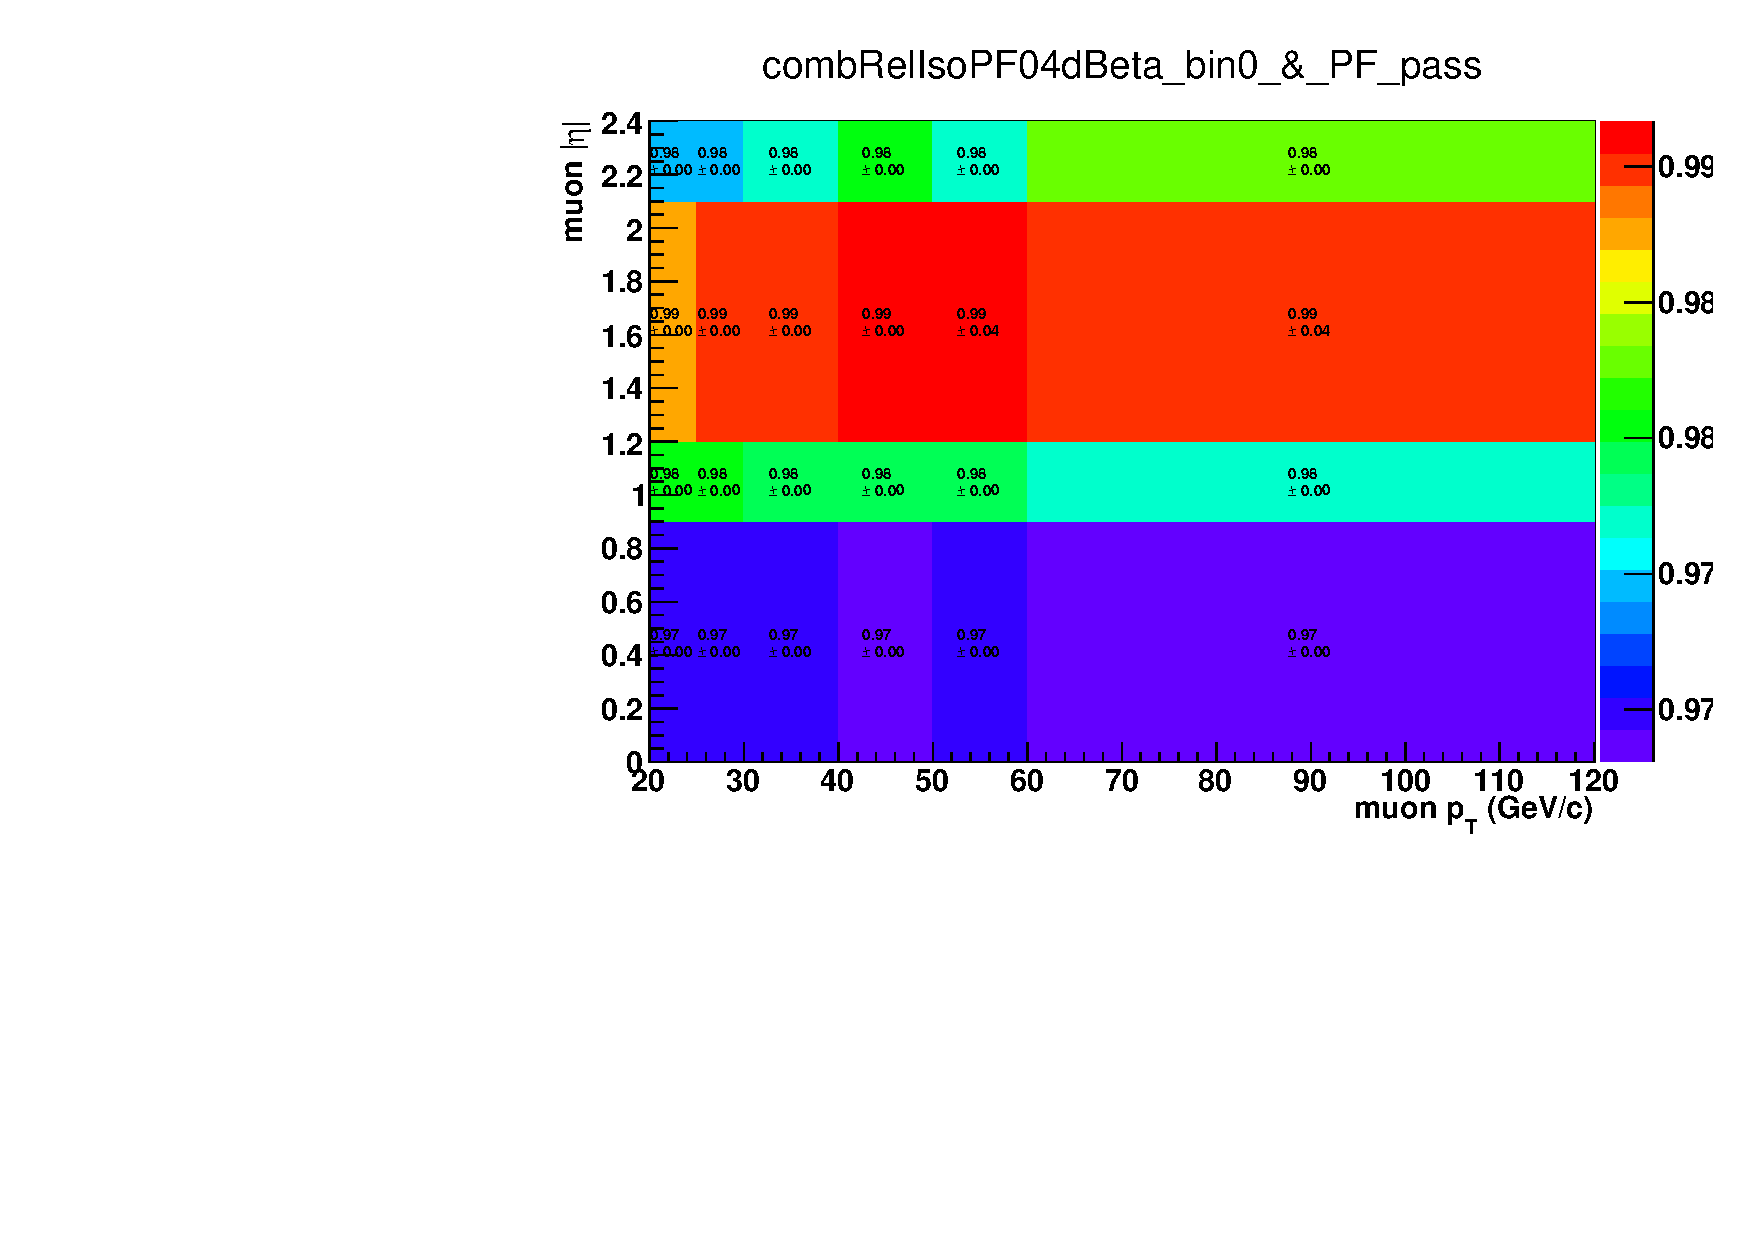
\includegraphics[width=0.475\textwidth]{trigger/Run_BCDEFG_PlotSF_hlt_Mu17_Mu8_OR_TkMu8_leg8_NUM_hlt_Mu17_Mu8_OR_TkMu8_leg8_DEN_LooseIDnISO_PAR_pt_eta_pt_abseta_ratio.pdf}
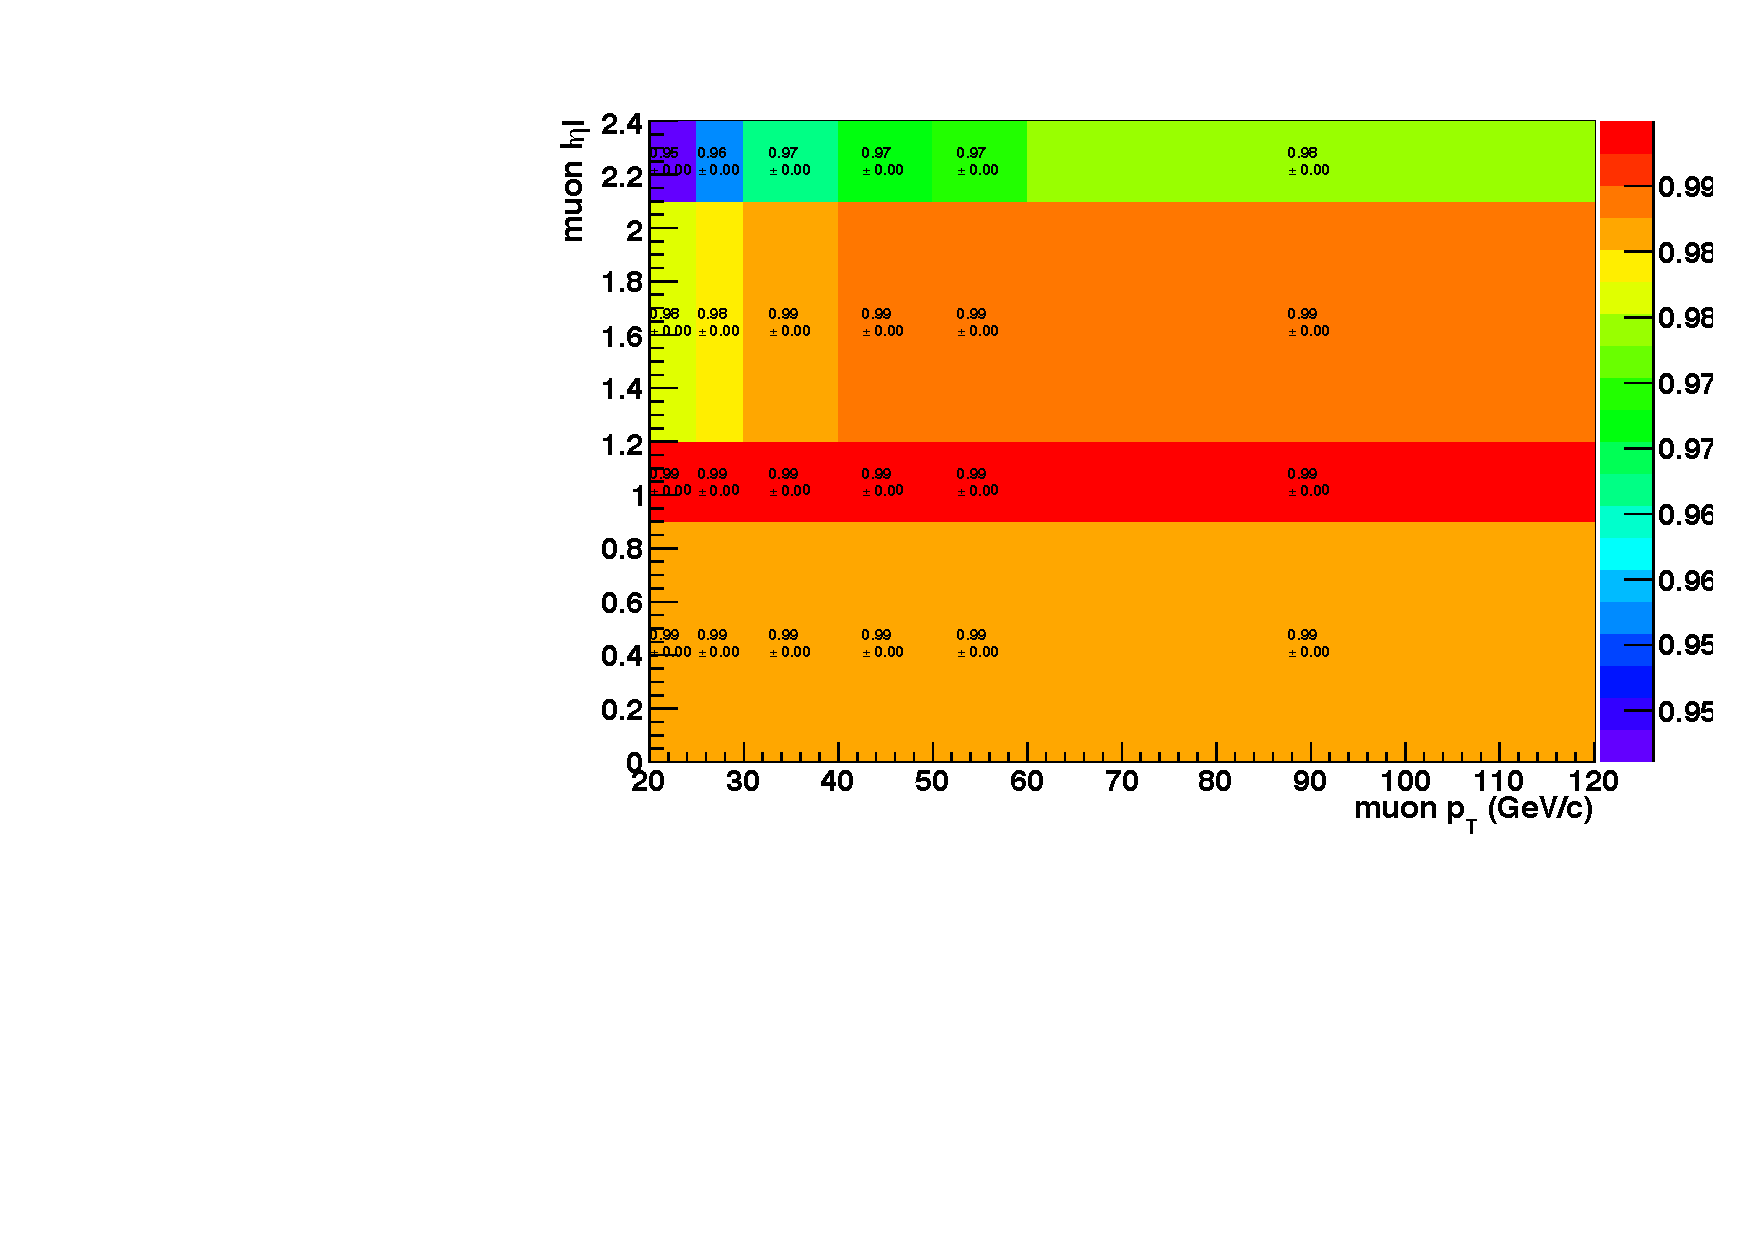
\includegraphics[width=0.475\textwidth]{trigger/Run_BCDEFG_PlotSF_hlt_Mu17Mu8_leg17_NUM_hlt_Mu17Mu8_leg17_DEN_LooseIDnISO_PAR_pt_eta_pt_abseta_ratio.pdf}\\
\caption[HLT SFs for muons as a function of $p_{T}$ and $\eta$, measured for eras B to G.]{Final HLT SFs for muons as a function of $p_{T}$ and $\eta$, measured for eras B to G. Left: Scale factors for 8 GeV leg (sub-leading muon). Right: Scale factors for 17 GeV leg (leading muons), provided that the sub-leading muon already passed the 8 GeV $p_T$ requirement.}
\label{fig:trigger_SF_dimu_BCDEFG}
\end{figure}

\begin{figure}[H]
\centering
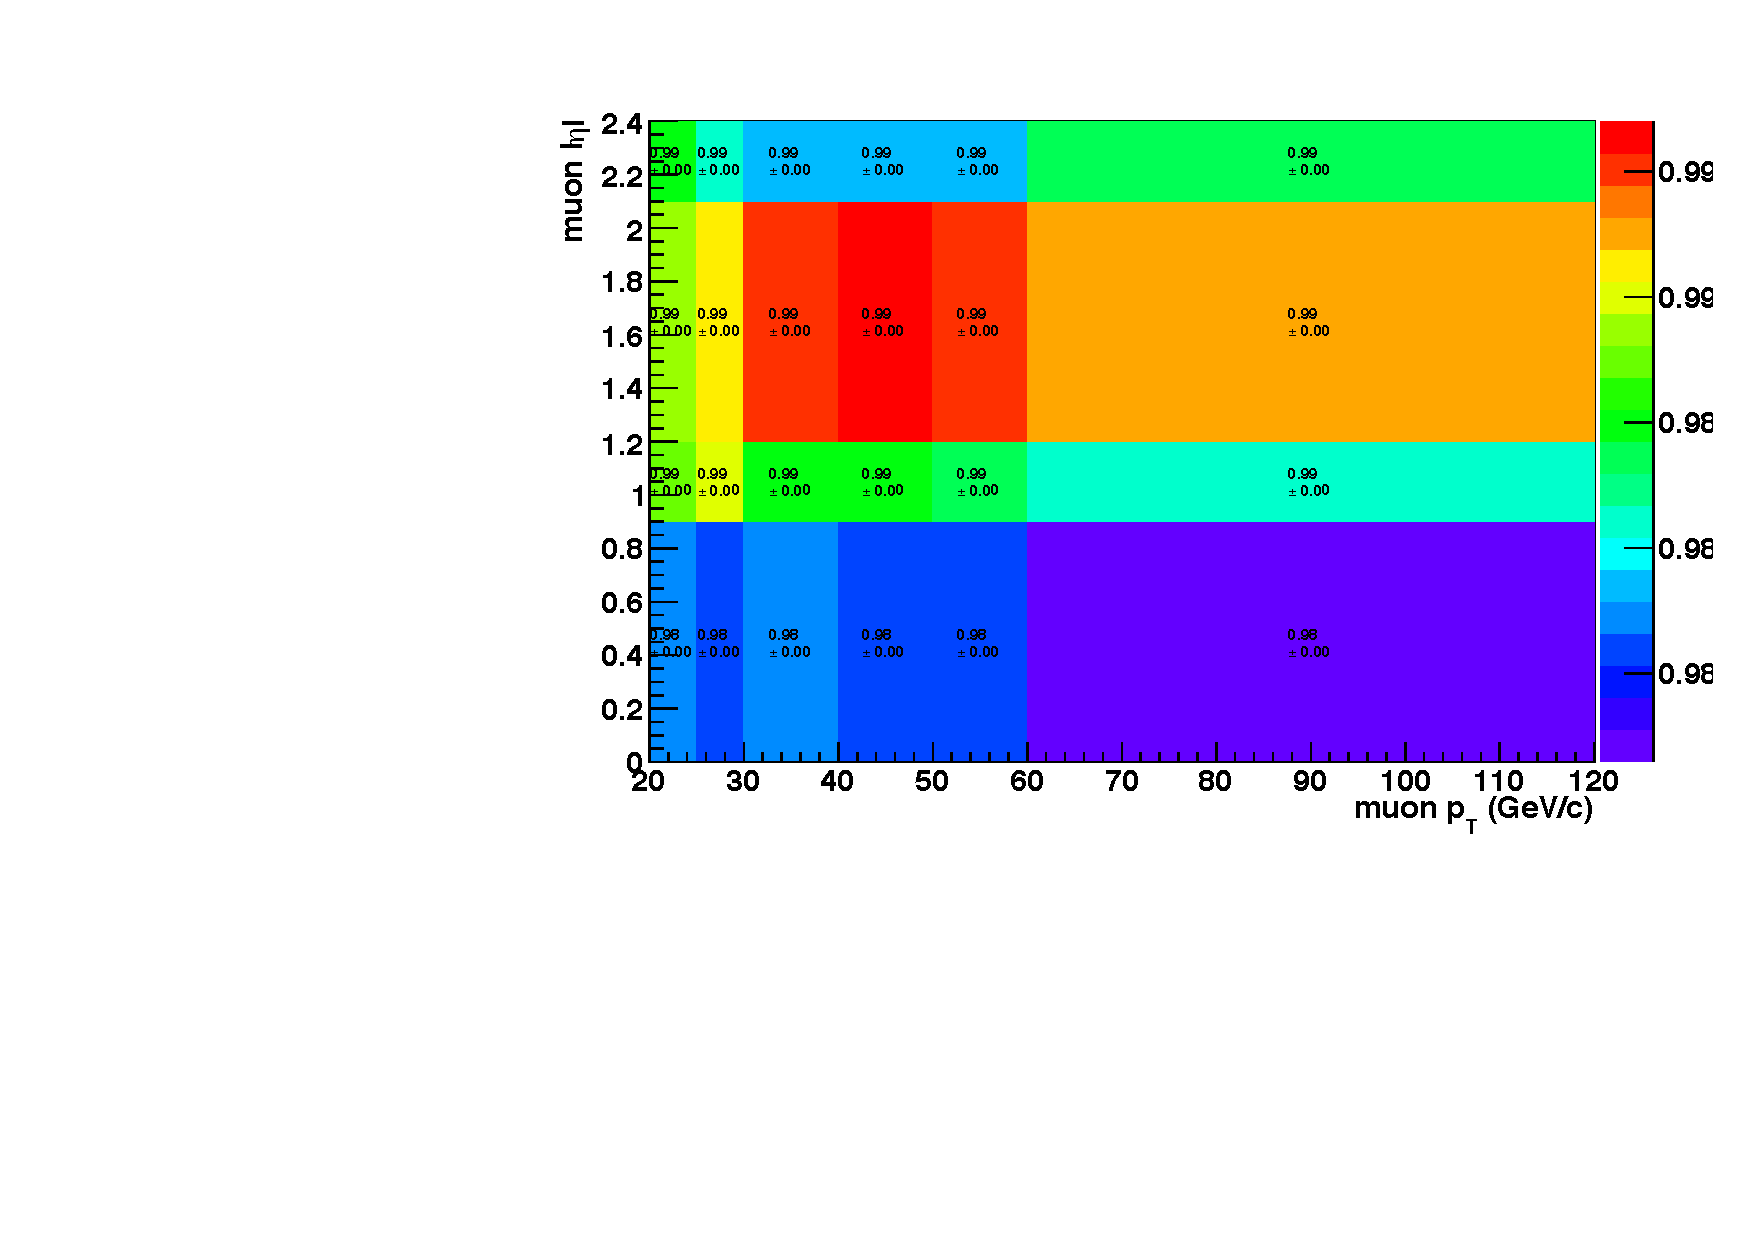
\includegraphics[width=0.475\textwidth]{trigger/Run_H_PlotSF_hlt_Mu17_Mu8_OR_TkMu8_leg8_NUM_hlt_Mu17_Mu8_OR_TkMu8_leg8_DEN_LooseIDnISO_PAR_pt_eta_pt_abseta_ratio.pdf}
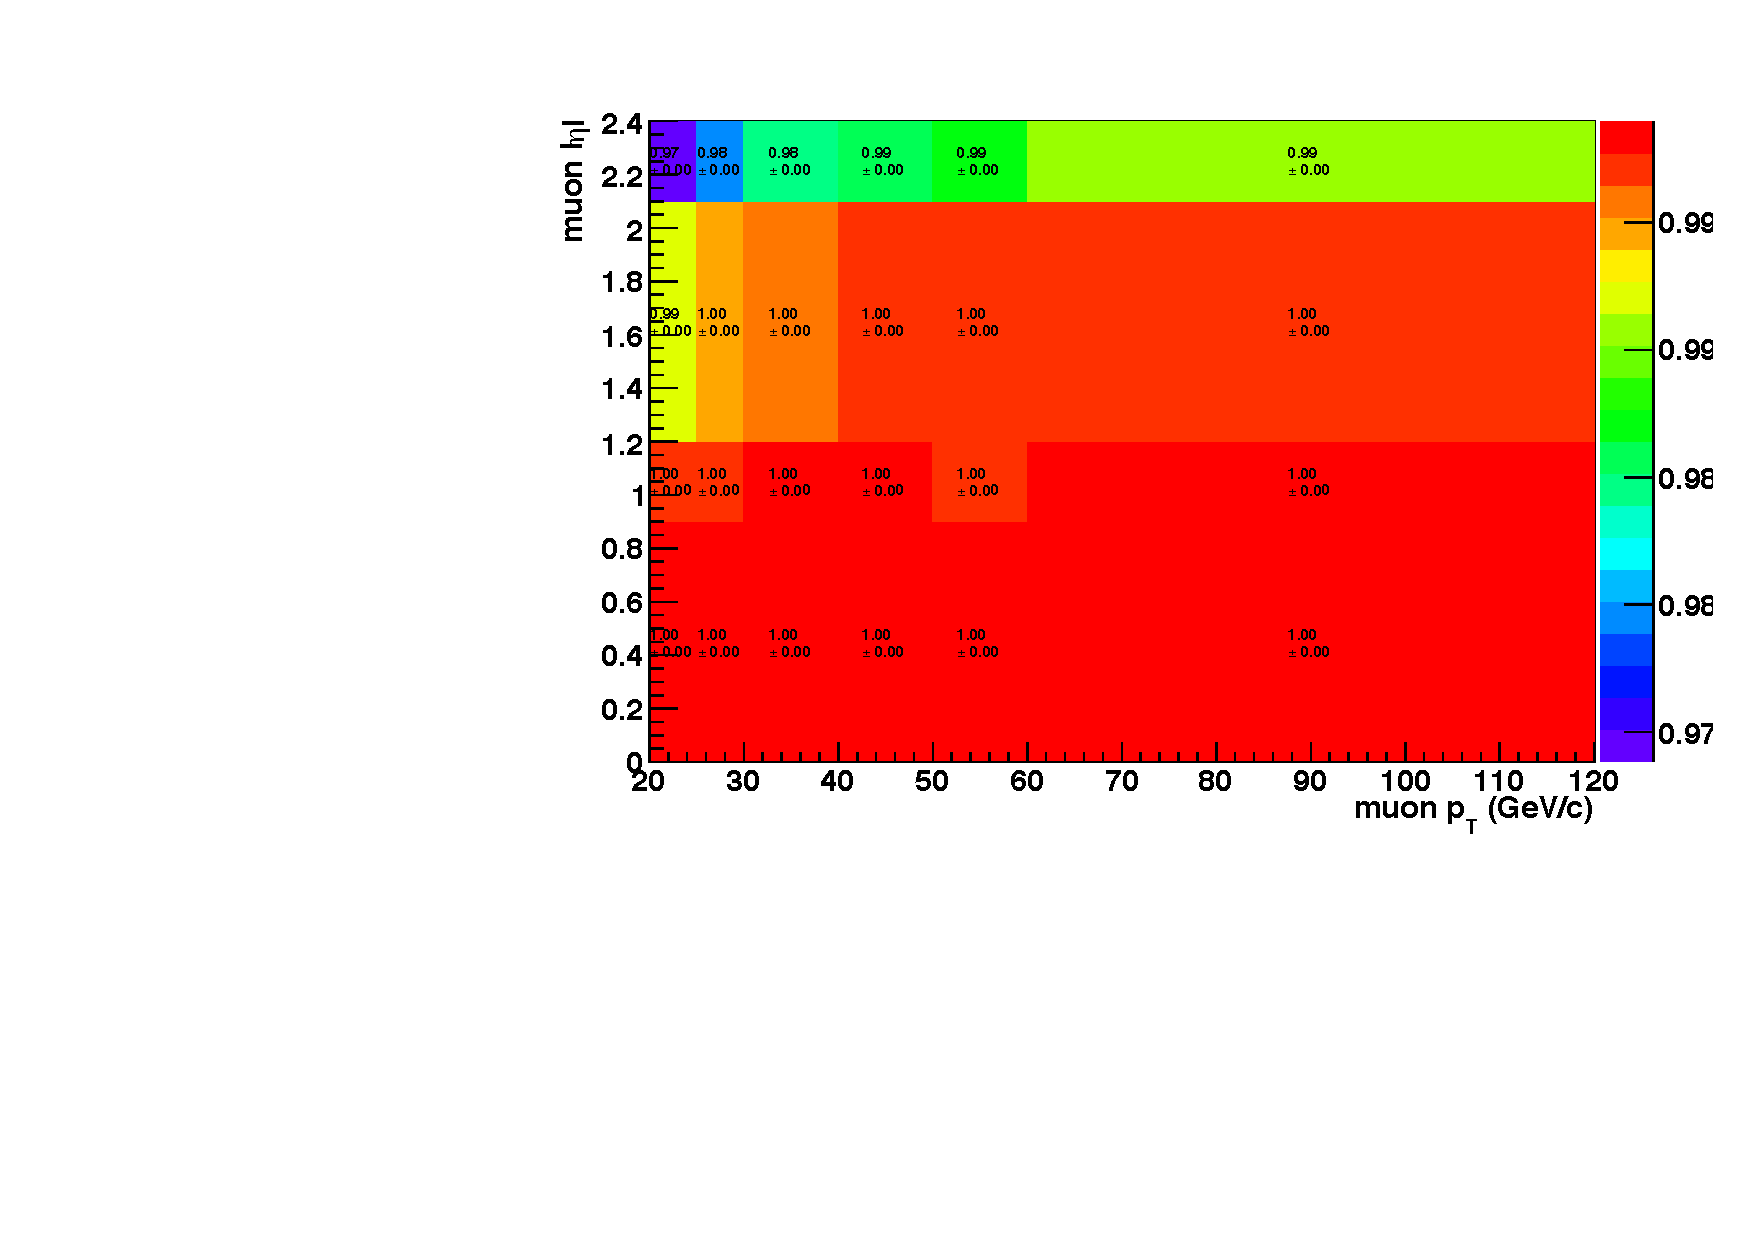
\includegraphics[width=0.475\textwidth]{trigger/Run_H_PlotSF_hlt_Mu17Mu8_leg17_NUM_hlt_Mu17Mu8_leg17_DEN_LooseIDnISO_PAR_pt_eta_pt_abseta_ratio.pdf}\\
\caption[HLT SFs for muons as a function of $p_{T}$ and $\eta$, measured for era H.]{Final HLT SFs for muons as a function of $p_{T}$ and $\eta$, measured for era H. Left: Scale factors for 8 GeV leg (sub-leading muon). Right: Scale factors for 17 GeV leg (leading muons), provided that the sub-leading muon already passed the 8 GeV $p_T$ requirement.}
\label{fig:trigger_SF_dimu_H}
\end{figure}

\begin{figure}[H]
\centering
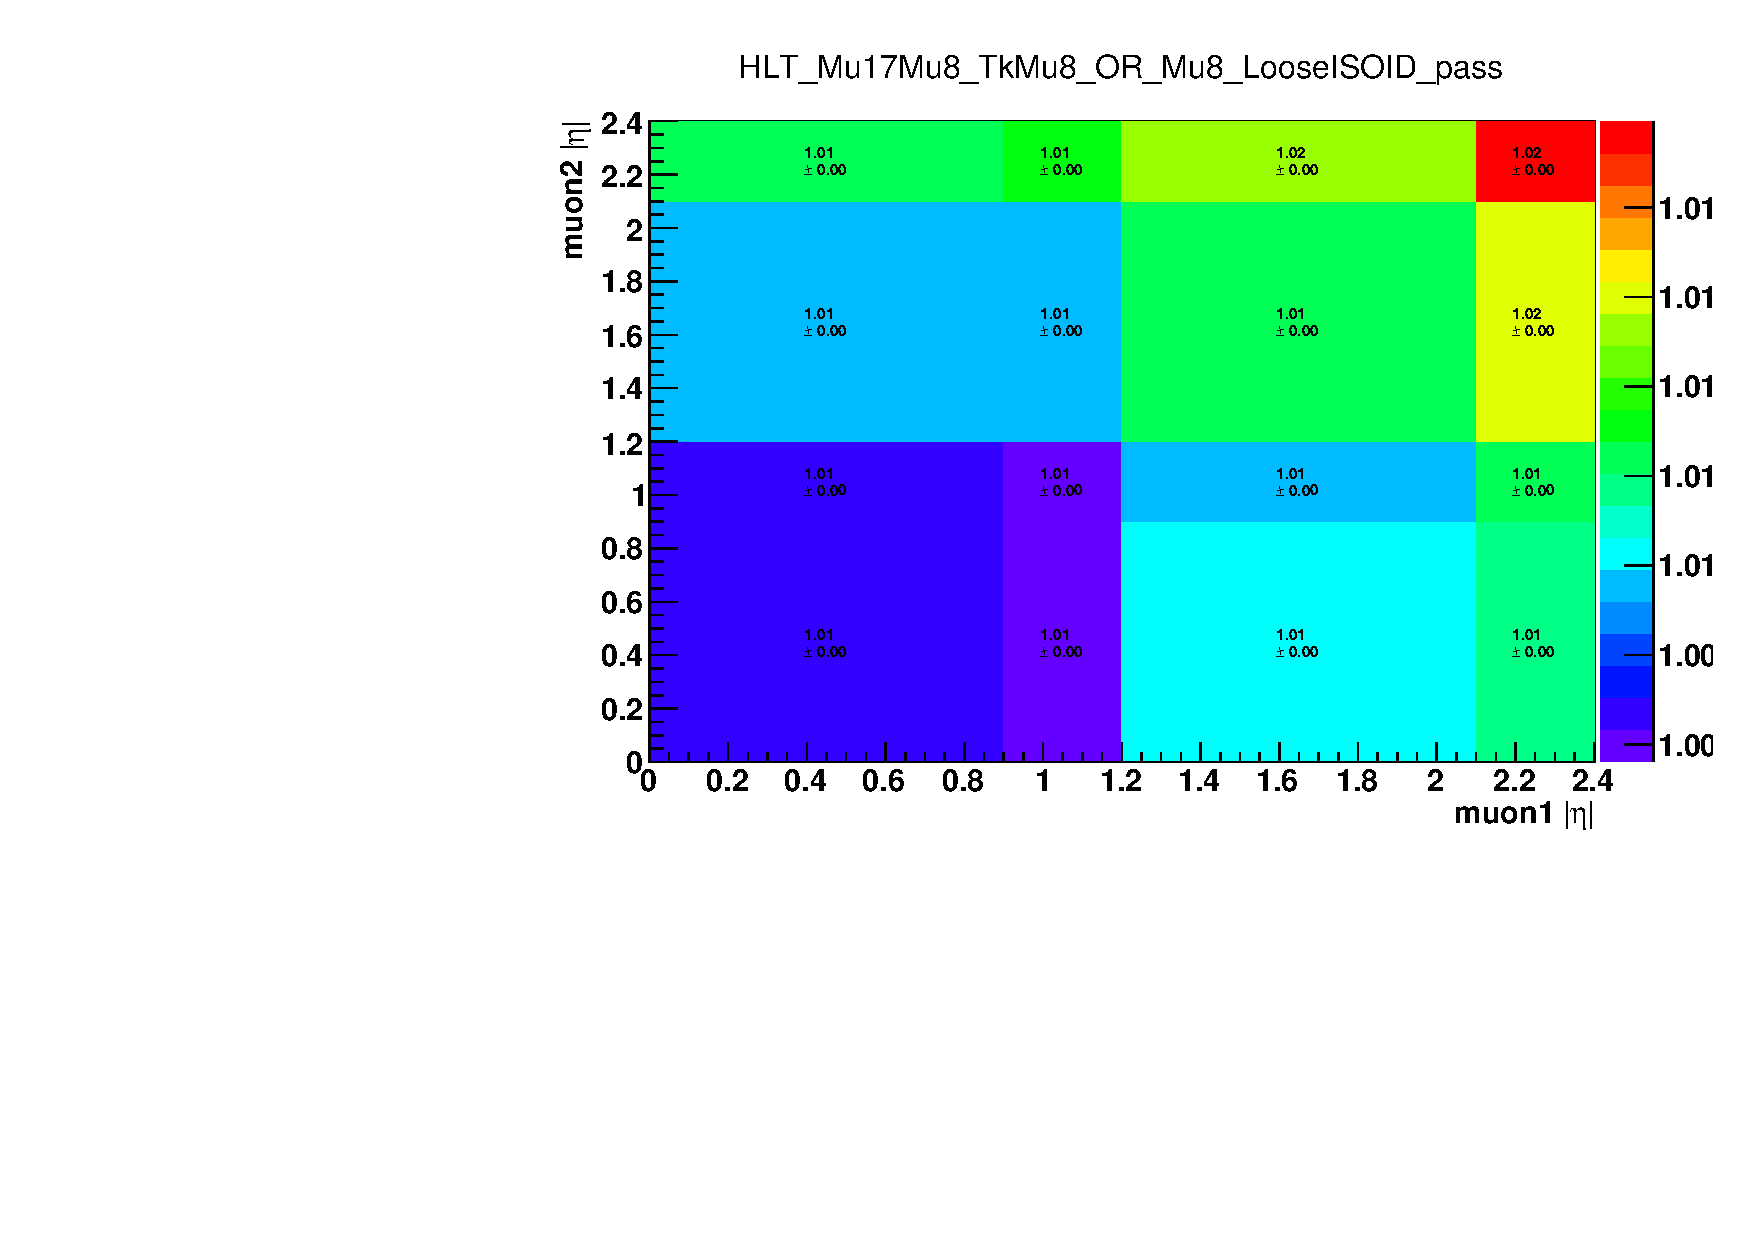
\includegraphics[width=0.85\textwidth]{trigger/PlotSF_dZ_NUM_dZ_DEN_hlt_Mu17_Mu8_OR_TkMu8_loose_PAR_eta1_eta2_abseta_tag_abseta_ratio.pdf}
\caption[SFs of the dZ requirement for muons.]{SFs of the dZ requirement for muons as a function of the $\eta$ values of both muons.}
\label{fig:trigger_SF_dimu_dZ_H}
\end{figure}

\section{Simulated Samples}
\label{sec:simulated_samples}

The data analysis carried out in this thesis is optimized using the MC simulation. MC samples for signal and background processes have been produced with various HEP software packages (``generators'') that generate the processes of interest: processes that create the final state of this measurement. 

\subsection{Signal processes simulation\label{sec:signalMC}}

The signal Monte Carlo (MC) samples have been generated using the {\MGMCatNLO} ~\cite{Alwall:2014hca} package. In these samples, the process of the gluon fusion production of WED spin-0 and spin-2 narrow resonances is simulated at leading order (LO). The production of resonances is followed by the decay of the resonances in the double Higgs boson system. All Higgs bosons are assumed to be SM Higgs bosons with an invariant mass of 125~GeV. Samples are generated for two spin hypotheses and 16 mass values covering the range of heavy resonance masses from 250 to 1000 GeV. Two types of signal samples are present: resonance decaying to $2b 2l 2\nu$ final state through the $X \rightarrow HH \rightarrow bbZZ$ decays and also through the $X \rightarrow HH \rightarrow bbWW$ decays. In both samples, the first Higgs boson decays to a pair of b quarks. However, in the first sample, the other Higgs boson decays to ZZ pair, while in the second sample the other Higgs boson decays to WW pair. Only \PZ~boson decays in a dielectron, a dimuon, or a two neutrino state are selected. For \PW ~bosons, the chosen signature is characterized by a W boson decay to an electron and an anti-electron neutrino or a muon accompanied by an anti-muon neutrino. Intermediate decays to tau leptons with the subsequent decays to electrons and muons are also included. 

To compare the expected numbers of events in the simulation to the number of observed events in the data for a given integrated luminosity, the signal production cross section has been normalized to 2 pb. This is a typical theoretical value of the production cross section of the WED particle in the 250-300 GeV range, the range to which the current physics analyses are very sensitive with the available LHC data. Additionally, the computed event rates take into account the branching fractions of the corresponding di-Higgs decay chains to the final state: 0.0012 and 0.0266 for $HH\to bbZZ\to bb\ell\ell\nu\nu$ and $HH\to bbWW\to bb\ell\nu\ell\nu$, respectively \cite{CERNYR4}.

\subsection{Background processes simulation\label{sec:bkgMC}}
In this analysis the main background processes are top-antitop production (\ttbar) and Drell-Yan production in association with jets. 
Other background processes that contribute to a lesser degree include single top production, diboson production, and the production of a single Higgs boson in association with a Z boson (``ZH production''), see Table \ref{tab:bg_mcsamples}. Other background processes are fully rejected in the event selection and thus are neglected. 

\begin{table}[H]
%\footnotesize
%\begin{center}
\caption[Background Monte Carlo samples.]{Background Monte Carlo samples. First column is the name of the process, the second column is the name of the generator used to simulate the corresponding process.
}
\label{tab:bg_mcsamples}
%\scalebox{0.8}{
\begin{tabular}{ | l | l | }%|l|r|r|r|r|r|} % it is separator L separator L separator and all with SPACES
\hline
% Sample & Generator & $m_{H} (\GeV/c^2)$ & $\sigma$ (pb) & events & $\int\cal L$ (\fbinv) \\
%\hline
%\multicolumn{5}{|l|}
{\texttt{DY plus 1 Jet }} & \MGMCatNLO-PYTHIA \\
% & \MADGRAPH\,5+\PYTHIA{}\,8 & 725 & 39 800 000 & 54.5 \\
%\multicolumn{5}{|l|}
{\texttt{DY plus 2 Jets }} & \MGMCatNLO-PYTHIA \\
% & \MADGRAPH\,5+\PYTHIA{}\,8 & 725 & 39 800 000 & 54.5 \\
%\hline
%\multicolumn{5}{|l|}
{\texttt{DY plus 3 Jets }} & \MGMCatNLO-PYTHIA \\
% & \MADGRAPH\,5+\PYTHIA{}\,8 & 394.5 & 19 400 000 & 50.2 \\
%\hline
%\multicolumn{5}{|l|}
{\texttt{DY plus 4 Jets }} & \MGMCatNLO-PYTHIA \\
% & \MADGRAPH\,5+\PYTHIA{}\,8 & 96.47 & 4 960 000 & 52.2 \\
%\multicolumn{5}{|l|}
{\texttt{WW }} & PYTHIA \\
% & \PYTHIA{}\,8 & 118.7 & 993 640 & 8.37 \\
%\hline
%\multicolumn{5}{|l|}
{\texttt{WZ }} & PYTHIA \\
% & \PYTHIA{}\,8 & 47.13 & 1 000 000 & 21.22 \\
%\hline
%\multicolumn{5}{|l|}
{\texttt{ZZ }} & PYTHIA \\
% & \PYTHIA{}\,8 & 16.523 & 985 600 & 59.65 \\
%\multicolumn{5}{|l|}
{\texttt{ZH with $H \to b\bar{b}$ and $Z \to \ell \ell$ }} & \MGMCatNLO \\
%\hline
%\multicolumn{5}{|l|}
{\texttt{$t\bar{t}$ }} & POWHEG-PYTHIA \\
% & \POWHEG+\PYTHIA{}\,8 & 831.76 & 187 626 200 + 97 994 442& 343 \\
%\hline
%\multicolumn{5}{|l|}
{\texttt{top quark tW channel }} & POWHEG-PYTHIA \\
% & \POWHEG+\PYTHIA{}\,8 & 35.6 & 1 000 000 & 28.09 \\
%\hline
%\multicolumn{5}{|l|}
{\texttt{$\bar{t}$ quark tW channel }} & POWHEG-PYTHIA\\
% & \POWHEG+\PYTHIA{}\,8 & 35.6 & 999 400 & 28.07 \\
%\hline\hline
%\multicolumn{5}{|l|}
{\texttt{top quark t-channel }} & POWHEG-PYTHIA \\
% & \POWHEG+\PYTHIA{}\,8 & 136*0.325 & 999 400 & 22.6 \\
%\hline
%\multicolumn{5}{|l|}
{\texttt{$\bar{t}$ t-channel }} & POWHEG-PYTHIA \\
% & \POWHEG+\PYTHIA{}\,8 & 81*0.325 & 1 695 400 & 64.4 \\
%\hline\hline
%\multicolumn{5}{|l|}
{\texttt{top quark s-channel }} & \MGMCatNLO-PYTHIA\\
% & \POWHEG+\PYTHIA{}\,8 & 10.32 & 998 400 & 96.74 \\
\hline%\hline
\end{tabular}
%\end{center}
%}
%\label{backgrounds} 
\end{table}

The Drell-Yan (DY) process in association with one to
four jets is generated at leading order (LO) using {\MGMCatNLO} with the MLM
matching scheme~\cite{Alwall:2007fs}. To account for the higher
order QCD and electroweak effects in V+jets production (following
~\cite{DY_QCDnEWK}), DY events are further reweighted
according to the dilepton transverse momentum, see \ref{DY_reweighting}. 

The simulations of the background processes associated with top
quark production are generated at next-to-leading order (NLO) in QCD. 
The {\POWHEG} ~\cite{Alioli:2009je, pwh1, pwh2, pwh3} generator was used to generate the
samples for top quark pair production and single top quark production in the tW
and t channels. For the single top s channel production, the
{\MGMCatNLO} generator was used. Single top backgrounds have been rescaled to the theoretical values of the next-to-next-to-leading order (NNLO) cross sections \cite{Kidonakis:2012db, Czakon:2013goa}. 

{\PYTHIA} 8.212~\cite{Sjostrand:2007gs, Sjostrand:2014zea} was used to generate diboson samples at LO. Diboson
background yields are normalized to NLO cross sections
\cite{CMS-PAS-SMP-18-002, CMS-PAS-SMP-16-006, Khachatryan:2016txa}. The dominant SM Higgs background process, the SM production of a single Higgs boson in the association with a \PZ ~boson (ZH), is simulated
at NLO using the {\MGMCatNLO} generator with FxFx merging ~\cite{Frederix:2012ps}. 
The SM Higgs background from the ZH process is scaled to NNLO with the
MCFM program ~\cite{Campbell:2010ff}. All the final cross section values at the NNLO accuracy in perturbative QCD have been computed with the original generators  ~\cite{xsecZH, xsecTT, xsecST, xsecVV}.

Normalizations for \ttbar ~and DY background processes are determined from data, as explained later in this chapter.

The NNPDF3.0 \cite{Ball:2014uwa} Parton Distribution Functions
(PDF) set is used for all the LO and NLO samples. {\POWHEG} and {\MGMCatNLO} are interfaced with
{\PYTHIA}8.212 for the parton
showering and hadronization stages. The description of the underlying event is done using the tune CUETP8M1 derived in \cite{Khachatryan:2015pea}. For the simulation of the CMS detector response, \GEANTfour~\cite{GEANT4} was used. 

For all MC simulations, further reweighting of events is done using the SFs derived to account for the discrepancies between the data and simulation. This includes SFs related to the lepton efficiencies as well as b tagging efficiencies, see Sections \ref{sec:TnP}, \ref{sec:b_tagging}.

As discussed in Section \ref{sec:pileup}, multiple overlapping proton-proton interactions occurred in each bunch crossing during data collecting in 2016, with an average of 24 hard scattering vertices per event. To account for this fact, all simulated samples include additional interactions to reproduce the real pileup distribution measured in data. To match the expected pileup in data, pileup reweighting is done for all MC simulated events.

\section{Physics Objects Selection}
\label{sec:objects}

\hyphenation{fa-shion}
\hyphenation{ener-gy}

During the reconstruction of the collisions at the CMS, data for each event are refined into high-level physics objects that correspond to particles created as a result of a proton-proton interaction. Among the physics objects necessary for this measurement are reconstructed electrons, muons, jets originating from quarks of heavy flavor (b jets), and the missing transverse momentum. The reconstruction details have been given in Section \ref{sec:cms_reco}. Here we focus on the analysis-specific selection of each of these physics objects.

\subsection{Electrons}\label{sec:electrons}
Electrons are reconstructed using the GSF algorithm \cite{GSF}. The electron candidates are then selected by first applying a loose isolation requirement of 0.4, after which they have to pass the Tight ID criterion defined by the CMS $e/\gamma$ POG, see \ref{sec:cms_reco}. At the offline level, the analysis applies additionally the loose WP (WP90) ~\cite{vhbbAN}. With this WP, one achieves an electron selection efficiency of 90\% by utilizing variables such as the agreement between the position of the ECAL cluster and GSF track that forms the electron, the energy of the 3 by 3 crystal core of the electron's cluster, the ratio of electron energy measured in ECAL to the electron's momentum measured in the tracking system, the ratio of the HCAL to ECAL energy, $p_T$ and $\eta$ of the electron, etc.
\subsection{Electrons}\label{sec:EGamma}

This is a justified level of the desired identification efficiency for the $Z \to \ell \ell$ channel since we select on-shell Z boson decays to charged leptons, where produced prompt leptons are very energetic. Finally, the electrons must be isolated from other particles in the event. Numerically, a selection criterion on the isolation is imposed (see Section \ref{sec:isolation}), where the expected contribution of particles from pileup interactions is $\rho$-subtracted using the effective areas method, see Section \ref{sec:isolation}. In this measurement, the isolation (with the cone size 0.3) for electrons is required to be smaller than 0.06, which means that all other particles together in the isolation cone around the electron cannot have more than 6$\%$ of the electron's energy.

\subsection{Muons}\label{sec:muons}
Muon candidates are reconstructed using tracker muon and global muon tracks identified by the PF algorithm. The selection procedure is similar to the one of electrons: first, a loose relative isolation selection of 0.4 is applied, then muons have to pass the Tight WP of the muon ID selection. At the offline level, a more stringent set of quality requirements (WP Loose) recommended by the CMS Muon POG is applied to the muon object. The ID definition contains the variables such as muon track segments compatibility, the fraction of valid hits in the inner tracker, $\chi^2$ variables of the inner tracker and global tracks, position matching variables, energy deposits in the calorimeters, impact parameter variables, etc. Lastly, a relative $\Delta\beta$-subtracted PF isolation selection of 0.15 is applied, with the cone size 0.4.

\subsection{Jets}\label{sec:jets}
Jets are reconstructed using the anti-$k_T$ jet clustering algorithm. This algorithm clusters PF candidates in a cone with a radius of 0.4. The energy and the resolution of the produced jets (so-called AK4 jets) are further corrected using JEC and JER corrections. These are used to calibrate the energy of the jets and to smear the resolution of jets to match the resolution of jets in the data. 

To reject misreconstructed (or misidentified) jets due to detector noise, pileup, etc., a loose jet identification WP is applied following the recommendations from the CMS JetMET POG. The ID variables include the jet $p_T$ and $\eta$, HCAL and ECAL energy fractions due to charged and neutral hadrons, the jet multiplicity, etc. If jets are found to be overlapping with charged leptons used in the measurement, these jets are not considered by the analysis. We consider jets with a $p_T$ greater than 30 GeV, which are in the range of $|\eta| < 2.4$. At least two jets must be present in the event. 

\subsection{b jets}\label{sec:bjets}
Each identified jet is further assigned a probability to originate from the b quark using the CMVA b tagging discriminant. This tagger produces as output a continuous discriminant with a value between -1 and 1, that is used to define three WPs depending on the chosen discriminant value. CMS BTag POG provides the CMS with the WP Loose, Medium, and Tight. For our measurement, the WP Medium requirement (>0.4432) has led to the best expected (from the simulation) results (the lowest upper limits as will be explained later). Therefore, the WP Medium is chosen in this analysis for the derivation of the final results. Jets passing the WP Medium requirement are classified as b jets. The threshold is chosen such that the misidentification rate for light-quark and gluon jets is about 1$\%$ and the b jet tagging efficiency for this working point is about 66$\%$. Two b jets with the largest scores of the CMVA discriminant are used to reconstruct the $H \to b\bar{b}$ candidate, which will be explained at length later in this chapter. 

\subsection{Missing transverse momentum}
In this measurement two neutrinos are present in the final state. They come from the off-shell Z boson decays to neutrinos and also from leptonic decays of W bosons. Even though the two neutrinos present in the signal events cannot be identified directly by the CMS detector, their presence can be inferred from the combined transverse momentum vector, using the momentum conservation requirement in the transverse plane for each event. The missing transverse momentum ~$\vec{p}^{miss}_T$ is computed as the negative vector sum of the transverse momenta of all visible PF objects and is further JEC and JER corrected, see Section \ref{sec:met}. The missing transverse energy \ETslash is the magnitude of the ~$\vec{p}^{miss}_T$ vector. 

All corrections recommended by the CMS JetMET POG are used in this measurement ~\cite{MissingETRun2Corrections}. Additionally, a set of filters related to the instrumental effects is employed, such as the removal of the misreconstructed signals in the HCAL, noise in the tracker, etc. ~\cite{MissingETOptionalFiltersRun2}. 

\section{Event Selection}\label{sec:selection}

The candidate events are selected in the data sample if they contain the following physics objects: 2 b jets, 2 charged leptons, and missing transverse energy. All these objects pass specific kinematic requirements defined in \ref{sec:cms_reco}, \ref{sec:triggers}, and \ref{sec:objects}. Then we reconstruct intermediate particles of the decay chain by combining the observed physics objects. $Z \to ll$ and $Z^* \to \nu \nu$ are reconstructed first. Then $H \to ZZ^*$ and $H \to b\bar{b}$ are reconstructed. The distributions of these variables will be shown later after the data-MC corrections are discussed. Finally, two Higgs boson candidates are used to form the $HH$ system that could originate from the narrow resonance we are searching for.

In this chapter, we discuss how $HH$ candidates are formed, how the selection criteria are applied to reduce contamination from background processes in the signal-enriched region (discussed later), how kinematic quantities used to compute the final results are defined, and how well simulation represents the collected data.

\subsection{Kinematic selection of physics objects}
We have described the kinematic selection of leptons and jets (and b jets) in the previous chapter. Because there is another $bbZZ$ measurement in the CMS Higgs group, our analysis shares some phase space with this other measurement. Therefore, the selected data samples may contain a certain overlap. The other $bbZZ$ team studies the $2 b 2 l 2 q$ final state, where $q$ stands for any quark initiating the jet. To ensure that both measurements produce statistically independent (``orthogonal'') results, a selection on the MET is introduced. Since the final results - the production cross sections multiplied by the BFs of the final state - depend on the mass point, the MET selection varies with mass. While the derivation of the final results (called ``limits'') will be explained later in this chapter, at this point it is worthwhile to point out that both analyses computed limits for all resonance mass hypotheses applying different MET selection criteria. Using a significance-like figure of merit ($S/(S+B)$), see Fig. \ref{fig:met_cuts}, we derived the set of MET requirements. These values have been checked by the other $bbZZ$ team and further optimized to yield the best simplified combined limits, when the results of both measurements are merged together. The final selection is shown in Table \ref{metCuts}.  %%%%Due to the computational intensity of such, a common value of the BDT threshold was chosen for some of the mass ranges. Here we show ``r vs cut'' figures. 

\begin{figure}[H]%hbpt? 
\begin{center}
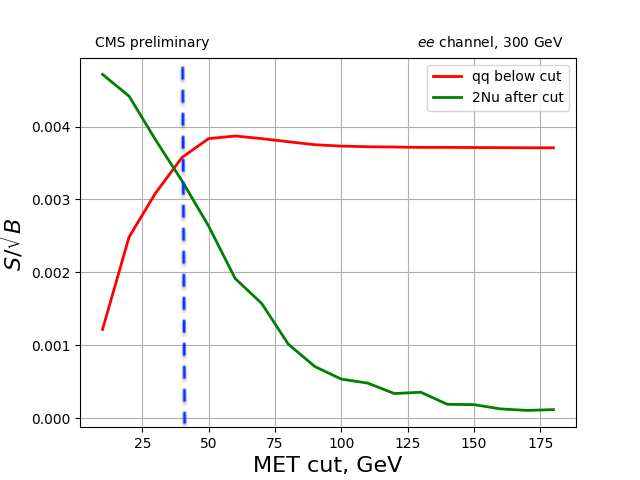
\includegraphics[width=0.45\textwidth]{ee_300_met_2.png}
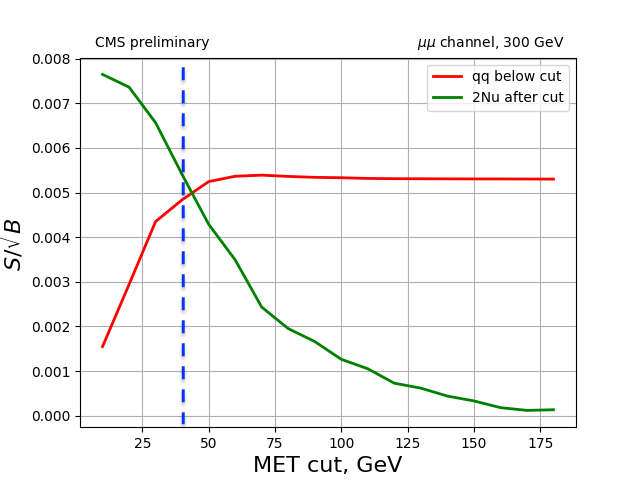
\includegraphics[width=0.45\textwidth]{mm_300_met_2.png}\\
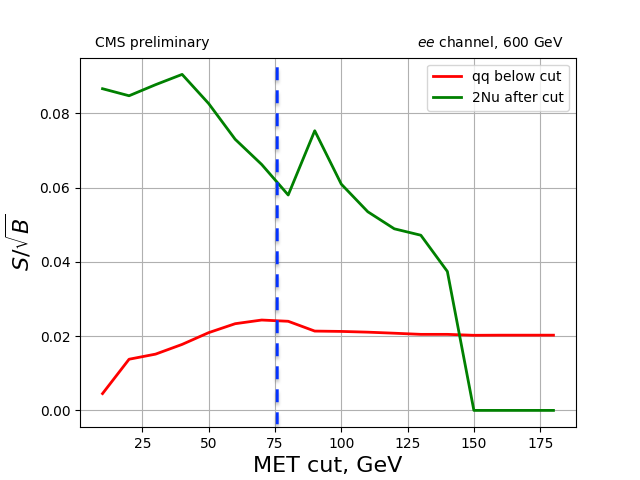
\includegraphics[width=0.45\textwidth]{ee_600_met_2.png}
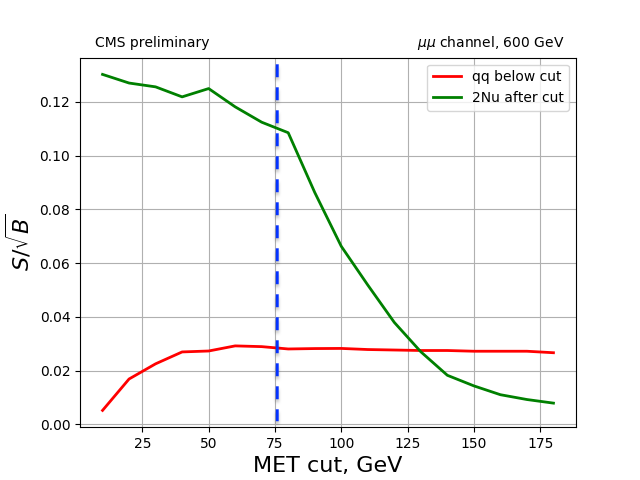
\includegraphics[width=0.45\textwidth]{mm_600_met_2.png}\\
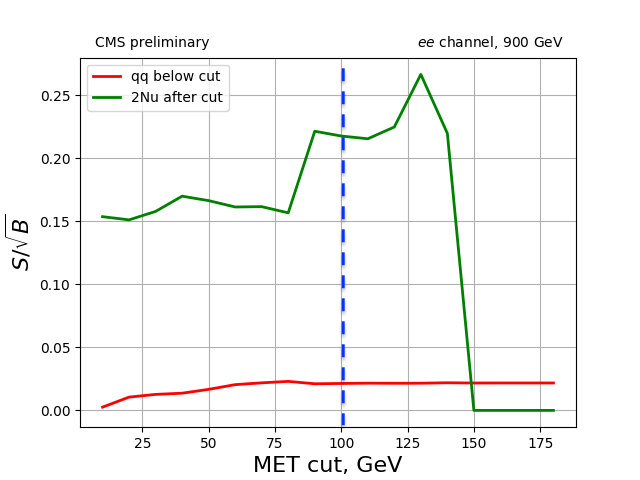
\includegraphics[width=0.45\textwidth]{ee_900_met_2.png}
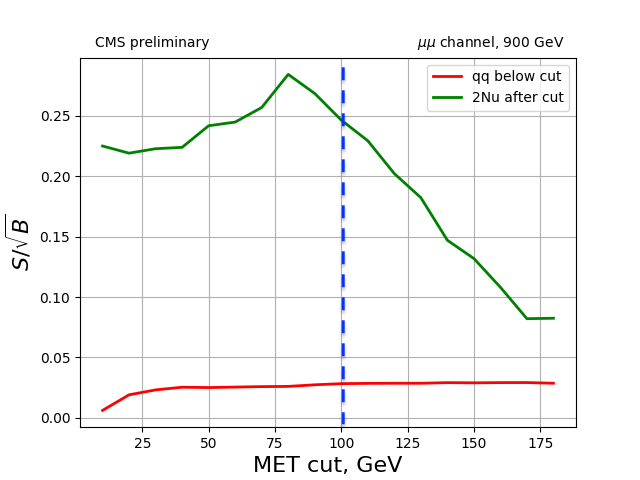
\includegraphics[width=0.45\textwidth]{mm_900_met_2.png}\\
\caption[Optimisation of the MET selection for two $bbZZ$ analyses]{ Optimisation of the MET selection for two $bbZZ$ analyses. S and B stand for signal and background process yields respectively. A significance-like figure of merit ($\sqrt{S}/B$) as a function of the MET cut is used to identify the best selection for each given mass hypothesis. The green curve shows the significance for this measurement, where events are kept above a given threshold. The red curve shows the  significance for the other $bbZZ$ measurement, where the MET requirement is inverted (events are kept below that threshold). Top: 300 GeV resonance mass. Middle: 600 GeV resonance mass. Bottom: 900 GeV resonance mass. The plots on the left are for the di-electron channel and the plots on the right are for the di-muon channel. The dashed blue lines indicate the values of the MET selection, see Table \ref{metCuts}.}
\label{fig:met_cuts}
\end{center}
\end{figure}

\begin{table}[H]
\begin{center}
\caption[The MET requirements as a function of the mass of the $HH$ candidate.]{The MET requirements as a function of the mass of the $HH$ candidate. Selection values (the second column) are provided for different mass hypotheses (the first column) of the narrow resonance decaying to the $HH$ system.}
\begin{tabular}{|c|c|} \hline
{Signal mass (GeV)} & \ETslash selection (GeV)\\\hline
260-300 & \textgreater~40 \\
350-600 & \textgreater~75 \\
650-1000 & \textgreater~100 \\
\hline
\end{tabular}
\label{metCuts}
\end{center}
\end{table}

\subsection{Signal candidate construction and selection}


Two leptons of the opposite signs and the same flavor with an invariant mass greater than 76 GeV are selected as Z candidates. This mass requirement helps to reject dilepton candidates not corresponding to real Z bosons. Events with a dilepton mass higher than 76 GeV will be used for SR and $t\bar{t}$ CR. Additional Z mass selection will be discussed later in this chapter. These on-shell Z bosons are assumed to come from the $H \to Z Z^*$ decays. The other Z boson, the off-shell Z boson, decays to two neutrinos in our signature and is represented by MET. The Lorentz four-vectors of the dilepton candidate and MET are added and the resulting four-vector represents the first Higgs boson candidate. 

The other Higgs boson is formed from the pair of b jets with the highest output value of the CMVA algorithm. No requirement is applied on the existence or absence of other b jets in an event because they may be present due to a b jet misidentification or b jets resulting from pileup interactions or the underlying event. The invariant mass of the \HBB~candidate is required to be greater than 20 GeV to remove contamination from background events with low mass resonances that decay to two jets, such as events with J/psi, Upsilon or low energy QCD interactions. There is no upper requirement on the \HBB~ invariant mass. Together with the first Higgs boson, the constructed di-Higgs system approximates the double Higgs boson production that this measurement studies. 

The final double Higgs boson candidate ($HH$ candidate) comprises the \Zll~candidate, the MET representing the \Znn~decay, and the \HBB~candidate. The four-momentum of this $HH$ candidate is defined as the sum of the four-momenta of the two leptons and two b jets in the candidate as well as the four-momentum of the MET defined as (\ETslash, $\vec{p}^{miss}_T$), see Sec. \ref{sec:cms_reco}.


$HH$ system decays to a pair of b quarks and a pair of W bosons can also result in the same final state. The expected yields for the $bbWW$ channel with respect to the $bbZZ$ yields are comparatively small (1 to 4) because of the stringent kinematic selection on the dilepton invariant mass. However, the contribution from the $HH$ system decaying through the $bbWW$ intermediate state is still considered to be part of our signal in this measurement. The minimum requirement on the dilepton mass is necessary to ensure that our measurement is orthogonal to the known $HH$ search from CMS in the $bbVV$ channel that focused on $bbWW$ decays \cite{bbWW}, where only events with the dilepton mass below 76 GeV were studied.

In collider physics, one of several common definitions of the transverse mass is given by: $M_T=\sqrt{( E^2- p_z^2)}$. This quantity is  used in CMS searches for new particles. We proceed in the same fashion constructing our final variable - \mTHH, using the di-Higgs four-vector defined in the previous paragraphs. 

While up until this moment we had the same requirements for the search of the radion/graviton $\to HH$ for any heavy resonance mass, it is worthwhile noting that at this point the analysis becomes mass point specific. This is because the selection on the BDT discriminant (which will be explained later) and the MET requirement differ with the mass hypothesis. When we compute limits for different radion or graviton hypotheses we apply different selection criteria. 

Finally, the reader should be informed that if an event does not have enough physics objects that are suitable (as discussed in the objects selection section) for building the \Zll~or \HBB~candidates, or if the event does not pass candidate selection requirements on those objects or the full $HH$ system, the event is discarded.

\subsection{Signal and control kinematic regions}

Three regions are defined: signal-enriched or signal region, and two CRs. The signal region is chosen such that the expected signal fraction is the largest there. Two control regions are defined such that they contain predominantly the background events with almost no signal. We define two CRs, one for each of the two main background sources: the CR for $t\bar{t}$ (CRTT) and the CR for Drell-Yan in association with jets (CRDY). The CRDY contains a high fraction of DY events, and the CRTT contains nothing but \ttbar~(more than 95\%). This ensures the correctness of the DY and \ttbar~normalizations extracted during the fit procedure (explained later).

Two intermediate particles in the decay chain are almost fully reconstructed, \HBB~and \Zll. The signal region is defined in the kinematic space of \HBB~and \Zll~events. This corresponds to an area determined by the mass of the Higgs boson (125 GeV) and the mass of the Z boson (91.2 GeV). To account for detector smearing effects, the mass windows near the pole masses are defined such that we select events within the \HBB~mass range from 90 to 150 GeV and Z mass range from 76 to 106 GeV, see Fig. \ref{fig:regions}. In  CMS, these relatively standard mass windows are chosen to take into account the detector resolution effects on a two b jet system and the dilepton mass (and the natural width for a Z boson), containing approximately 95$\%$ of true Higgs and Z boson candidates. The proportion of signal events is further increased with respect to background events by applying an additional requirement, the MVA requirement, which will be explained in the next section.

\begin{figure}[!htb]%hbpt? 
\begin{center}
%\raisebox{0.17\height} 
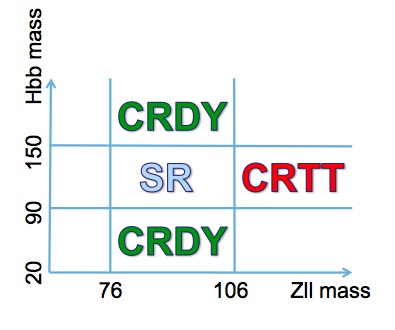
\includegraphics[width=0.45\textwidth]{regions.png}
\caption[Analysis phase space with the signal and two control regions.]{ Signal region, control region \ttbar, and control region Drell-Yan in the kinematic space of \ZtoLL ~and ~\HBB~masses. }
\label{fig:regions}
\end{center}
\end{figure}

CRs are defined by inverting the SR selection. The Drell-Yan plus jets (or ``DY'' later for brevity) background process contains a real Z boson with two jets. Two jets from this process have a broad distribution. We obtain the CRDY by inverting the \HBB~selection. To construct the CRTT, we use the fact that $t\bar{t}$ events do not contain a real Z boson. Thus, to define CRTT, we invert the \Zll~selection and use only the events in the upper range of the Z mass, see Fig. \ref{fig:regions}. 

CRs are used to fit the event yield of the simulated background processes to the event yield in data and, thus, to determine the relative normalizations of $t\bar{t}$ and Drell-Yan background processes, which is done using CRTT and CRDY correspondingly. 

The efficiency of the candidate selection, up to this point, is summarised in Table \ref{eff_upto_bdt}, where numbers are provided for the SR. The number of observed data events and expected signal events will be presented in the Section \ref{sec:statistics}. The signal contributions are split into two components: $bbZZ$ and $bbWW$, and are shown separately. The corresponding total number of events passing the selection are also given, shown in the fourth column. Note that the number of signal events surviving the BDT selection in the SR is 2 - 5 times greater (depending on the mass point) than the number of all signal events present in the CRDY, while CRTT contains no signal. 

\begin{table}
\begin{center}
\caption[Fraction of events surviving the candidate selection and kinematic requirements.]{Fraction of events surviving the candidate selection and kinematic requirements. Efficiencies are given for $bbZZ$ and $bbWW$ contributions in the SR and are normalised to the initial event counts before any selection is applied. A di-muon channel is presented. Numbers for the di-electron channel have the same trend but lower values, because in CMS efficiencies for electrons are lower than for muons.}
\begin{tabular}{ |c|c|c| } \hline
{Process} & Mass (GeV) & Efficiency (\%)  \\\hline
bbWW & 300 & 0.2 \\
bbZZ & 300 & 10.4 \\\hline
bbWW & 900 & 0.1 \\
bbZZ & 900 & 15.1 \\\hline
\end{tabular}
\label{eff_upto_bdt}
\end{center}
\end{table}

\subsection{Signal region candidate selection with a multivariate technique}

After the SR and CRs have been defined, in the final step of the event selection we require the events in the SR to pass the threshold value of the BDT discriminant. An MVA discriminant that uses a boosted decision trees algorithm is trained considering a number of kinematic quantities of a candidate to be above a certain threshold. As this selection step is complex, it is described in a dedicated chapter (see \ref{sec:BDT}).

\subsection{Candidate reweighting in simulated events}

Several factors lead to a difference in the behavior of simulation in comparison to real data. These factors include the difference in the kinematics of simulated events from what it is in nature as well as the differences in the simulation of the detector response that affects reconstruction efficiencies for physics objects that form candidates, as well as tagging and mistagging rates for b jets. 

These factors are quantified through per-event SFs that are used as event weights in preparation of all kinematic distributions and computation of the expected event counts. The SFs of all types are produced centrally in CMS by the appropriate POGs. The full per-event weight for a simulated event is a product of all individual SFs discussed below.

\begin{itemize}

\item{\bfseries Lepton efficiency} 

Scale factors that reflect the differences between data and simulation in lepton 
reconstruction, selection, and triggering are computed as the ratios of the corresponding
efficiencies between data and simulation. Additionally, since the DZ requirement was absent for some triggers, the efficiency of the DZ selection needs to be measured. 

The efficiencies and, subsequently, the scale factors are measured separately for the efficiencies of the reconstruction procedure, lepton identification, isolation requirements, and impact parameter requirements. The TnP procedure discussed in Section \ref{sec:TnP} is applied to measure all of these efficiencies. The scale factors of all listed types for both leptons are used as multiplicative factors
to form the per-candidate lepton efficiency SF.

On average, the muon ID scale factors are equal to 0.992 - 1.004, depending on the $p_t$ and $\eta$ of leptons. The muon ISO SFs are equal to 0.991-1.004. The electron ID $\cdot$ ISO SFs, computed together, are ranging from 0.832 to 1.073. For an an illustration, see the Fig. \ref{fig:eleIDnISO_SF}. The HLT SFs have been discussed in the subsection \ref{sec:triggers}. 



%\begin{figure}[H]
%\centering
%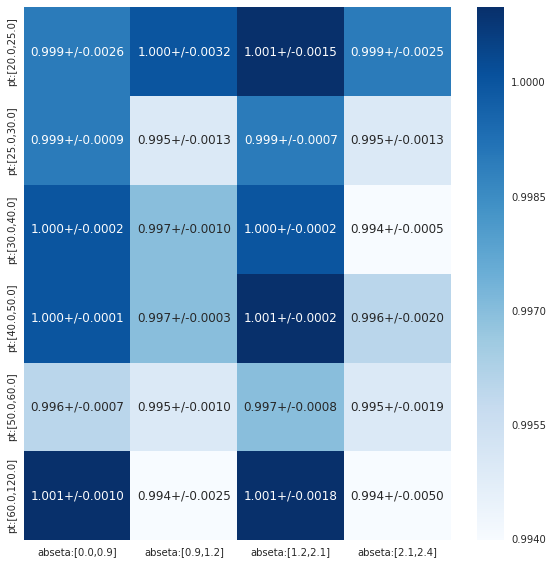
\includegraphics[width=0.55\textwidth]{muon_ID_BCDEFv2.png}
%\bigbreak
%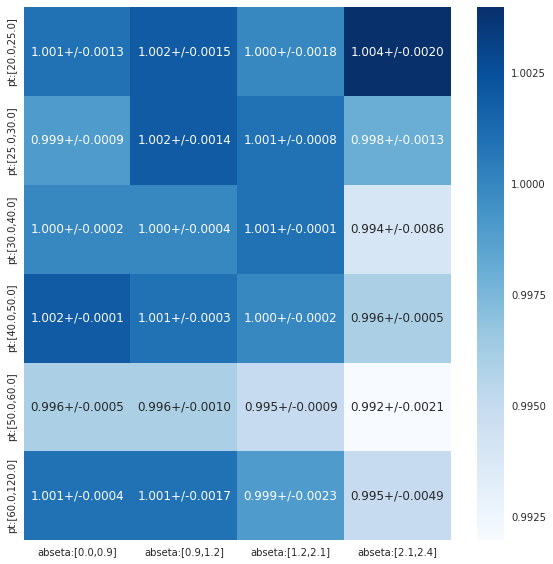
\includegraphics[width=0.55\textwidth]{muon_ID_GHv2.png}
%\caption[Muon ID scale factors as a function of the electron $p_{T}$ and $\eta$.]{ Muon ID scale factors as a function of the muon $p_{T}$ and $\eta$. Top: eras B to F. Bottom: eras G and H.}
%\label{fig:muonID_SF}
%\end{figure}
%
%
%\begin{figure}[H]
%\centering
%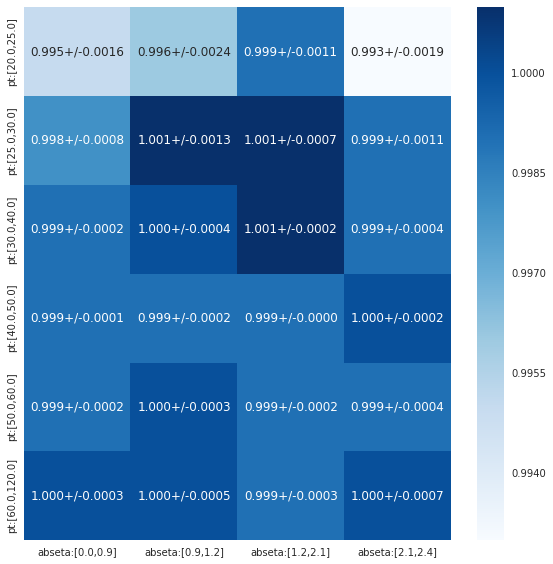
\includegraphics[width=0.55\textwidth]{muon_ISO_BCDEFv2.png}
%\bigbreak
%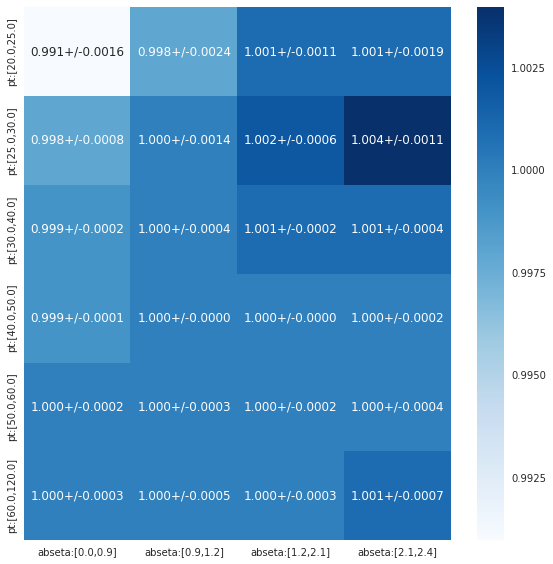
\includegraphics[width=0.55\textwidth]{muon_ISO_GHv2.png}
%\caption[Muon ISO scale factors as a function of the electron $p_{T}$ and $\eta$.]{ Muon ISO scale factors as a function of the electron $p_{T}$ and $\eta$. Top: runs B to F. Bottom: eras G and H.}
%\label{fig:muonISO_SF}
%\end{figure}

\begin{figure}[H]
\centering
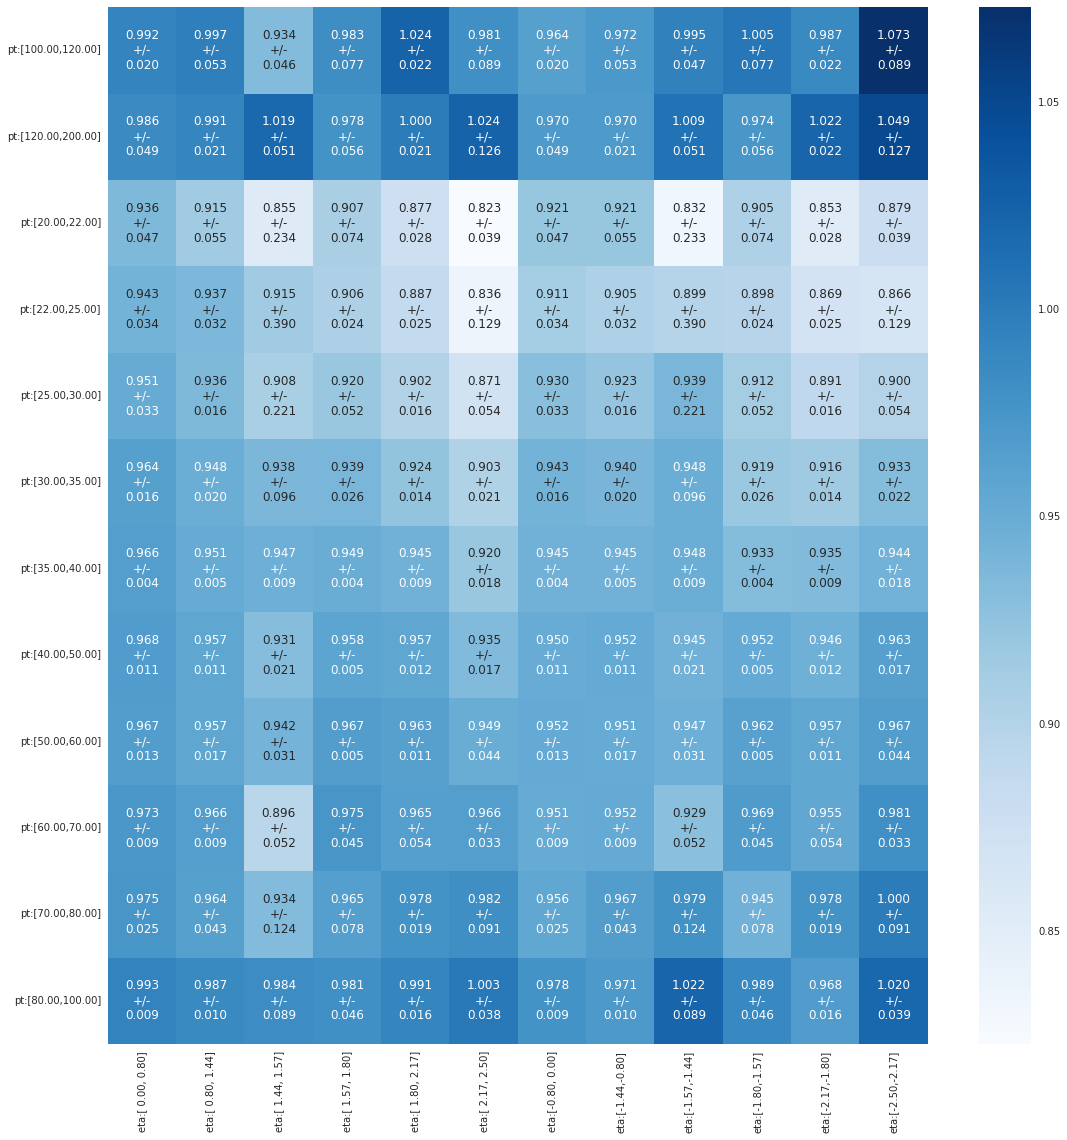
\includegraphics[width=0.8\textwidth]{EIDISO_ZH_out.png}
\caption[Electron ID plus ISO scale factors.]{ Electron ID plus ISO scale factors as a function of the electron $p_{T}$ and $\eta$. The x axis corresponds to $\eta$ of the electron, the y axis corresponds to $p_T$ of the electron.}
\label{fig:eleIDnISO_SF}
\end{figure}




\item{\bfseries b tagging and light flavor mistagging probability scale factors} 

To identify the b jets, a selection on the output of the CMVA tagger is applied. The efficiency of the b jet selection is measured (with the TnP method) in data and in the heavy-flavor enhanced MC sample, the $t\bar{t}$ process containing top and anti-top quark decays. Since these efficiencies are different, the b tagging SFs are derived. Because this measurement contains two b jets in the final state, a total per event b tagging SF is equal to 0.7 - 1.3 for signal and 0.6 - 1.4 for background processes. 

\item{\bfseries Kinematic reweighting of the DY plus jets samples} 
\label{DY_reweighting}

DY plus jets samples used in this measurement are produced at LO (see Section \ref{sec:data_and_triggers}). The samples are corrected to exhibit NLO kinematic behaviour in the EW interaction by assigning a weight to each event. As the biggest discrepancy between data and simulation for such samples is typically found in the di-jet invariant mass distribution, an LO-to-NLO correction as a function of the $\Delta \eta_{b\ jets}$ separation is computed following the procedure described in \cite{DYLOtoNLO}. As stated there, this correction improves the data-MC agreement in many distributions derived from the di-jet objects or based on the $p_T^{\Zll}$ variable, while has a negligible effect on the remaining kinematic variables. The correction means that a kinematic weight is assigned to each event.

It was found by several Higgs analysis teams that the previous correction does not address the data-MC discrepancies for Z bosons with high $p_T$. The spectrum of the $p_T$ of the Z boson distribution is harder for DY plus jets MC simulation than for data. This is due to the fact that the simulation does not include higher-order QCD+EW corrections \cite{NLO_Vjets}. The DY plus jets simulated samples are reweighted as a function of the $p_T^{\Zll}$ to update the LO samples to the NLO in QCD+EW. The corrections can be as large as 10\% for energetic Z bosons with $p_T > 400$ GeV.

\end{itemize}

\section{Multivariate selection in the signal region}

To reduce the background contamination in the SR, we employ an MVA discriminant. In this section, we will discuss which discriminating variables were used, how the MVA discriminant was constructed, and what the efficiencies of the BDT selection are for all major signal and background processes. 
\label{sec:BDT}

\subsection{Kinematic variables of a candidate}
\label{sec:variables}

A number of kinematic quantities can be constructed out of four-vectors that are used to construct candidates of our final state. The distributions of these quantities, in general, differ for candidates originating from different background processes as opposed to for candidates from the hypothetical signal. 

In this section, we discuss a set of kinematic quantities that are the most discriminating between the expected signal candidates and background candidates. This set of variables is used as an input for computing the multivariate discriminant that is later discussed in this section. In total, nine variables are chosen for this purpose. About 30 - 40 other kinematic variables were considered at the early stages of this data analysis. However, they were discarded as it was found that they do not improve the results of this measurement in a significant way, while at the same time they considerably increase the complexity of the measurement.

Since the MVA selection requirement will be applied on a quantity that was computed based on these variables, the simulation has to reproduce the variables well. We will define each of the nine variables below. For SR and both CRs, we will show the comparison of distributions from data and simulation for each variable. Since the number of plots would be too large to show for two channels and two spin hypotheses, not to mention for all masses, we will include in this dissertation only di-muon channel plots for the 300 GeV graviton mass hypothesis. However, all other relevant figures of the nine main variables, including the di-electron channel and other mass points, were examined and documented in the internal CMS notes, and show similar behavior and agreement as those included here.

As we outlined before, even for simple physics objects the distributions from MC simulations and collected data have discrepancies. For more complex objects and candidates, these discrepancies become even larger. In general, MC simulations do not reproduce very narrow regions of the kinematic phase space well, or align with the data perfectly at the high order of the QCD. Therefore, one normally adjusts the event yields (rates) of background processes using the normalization values determined in the fit to data in the control regions. The shape of the distributions are further modified during the bin-by-bin correction procedure. The distributions as they are, without the extra normalizations from the fit being applied to the event yields of MC simulated background processes, are called pre-fit distributions. After the normalizations from the fit are applied to the rates of background processes, post-fit distributions are obtained. In the next Section, we provide both pre-fit and post-fit distributions back-to-back for an illustration how MC simulation performs out of the box and after the adjustment based on the fit to the data. The fitting procedure is discussed at length in the Statistical Analysis chapter \ref{sec:statistics}. 

The list below summarises the set of variables used as input to the MVA discriminant:

\begin{itemize}

\item{\bfseries $\Delta R$ separation between two b jets.}
The $\Delta R$ (defined in Section \ref{ch:cms}) separation between the b jets ($\Delta R_{b\ jets}$) gradually decreases as we start considering larger graviton or radion masses. This fact is explained by the Lorentz boost of the \HBB~system. When a heavy resonance produces two SM Higgs bosons, they are highly boosted. For the Higgs boson, which will further decay to a pair of b quarks (\HBB), the b quarks will come out of the decay almost collinear to each other with a minimal value of $\Delta R_{b\ jets}$. For background processes, this separation does not depend on the graviton or radion mass. 

\item{\bfseries $\Delta R$ separation between two leptons.}
The distance between two leptons in $\eta - \varphi$ space ($\Delta R_{leptons}$) tends to be smaller for the dilepton system coming from the real Z bosons originating from \HZZ~decays, in comparison to the $\Delta R_{leptons}$ distance between two random OSSF leptons produced by background processes. 

\item{\bfseries Missing transverse momentum.}
The $\vec{p}^{miss}_T$ distribution coming from the off-shell Z bosons is constrained by the invariant mass of the parent Higgs boson and, thus, has a more narrow distribution. Conversely, the MET coming from $t\bar{t}$ background process can produce smaller and larger values of the MET outside of the aforementioned constrainment. 

\item{\bfseries Invariant mass of the $\HBB$~candidate.} 
The mass of a two b jet system coming from a real Higgs boson tends to be close to the SM Higgs boson invariant mass smeared by the b jet energy-momentum resolution, while the background candidates from unrelated b jets can have smaller and larger masses, especially if they come from the top quarks of the $t\bar{t}$ background.

\item{\bfseries Transverse momentum of the \HBB~candidate.} 
The transverse momentum of the \HBB~candidate ($p_T^{Hbb}$) tends to have a relatively narrow and peaked distribution for candidates coming from the hypothetical signal in comparison to the broad distributions produced by background processes. 

\item{\bfseries Invariant mass of the $ZZ^*$~system.} 
$ZZ^*$ mass of two Z bosons coming from the Higgs boson decay ($\HZZ$) tends to be close to the SM Higgs boson mass smeared by the $\vec{p}^{miss}_T$ resolution, while the background candidates from DY production in association with jets can have random masses. These can be particularly large if they come from DY production in association with several jets in addition to some instrumental MET present in the event.

\item{\bfseries Transverse momentum of the $ZZ^*$~system.} 
The transverse momentum of the \HZZ~candidate ($p_T^{Hzz}$) tends to have a relatively narrow and peaked distribution for candidates coming from the hypothetical signal in comparison to broad distributions produced by the background processes. 

\item{\bfseries Invariant mass of the Z boson candidate.} 
Z bosons coming from the Higgs boson have the invariant mass near the pole mass, while \ttbar contains no real Z bosons.

\item{\bfseries Transverse momentum of the Z boson candidate.} 
The transverse momentum of the Z candidate ($p_T^Z$) tends to have a relatively narrow distribution for candidates coming from a real Z boson produced in the decays of the hypothetical signal in comparison to broad distributions of $p_T^{\ell\ell}$, when dilepton systems are produced by background processes. 

\end{itemize}

At this stage of the analysis description, we refer the reader to the pre-fit plots (figures in the left columns). The figures are shown in the following order: all nine distributions in CRDY (see Figs. \ref{MCcomparisons_mm_low_CRDY_1}, \ref{MCcomparisons_mm_low_CRDY_2}, \ref{MCcomparisons_mm_low_CRDY_3}, \ref{MCcomparisons_mm_low_CRDY_4}, \ref{MCcomparisons_mm_low_CRDY_5}), in the BDT sideband \footnote{Once the BDT selection is introduced, in the SR the candidates will have to pass the BDT requirement. The region below the BDT selection is called the BDT sideband. In the unblinding scheme employed in this measurement, discussed later, the SR distributions are not examined at this point; data-MC agreement is checked using CRs and the BDT sideband of the SR.} of the SR (see Figs. \ref{MCcomparisons_mm_low_SR_bdt_sideband_1}, \ref{MCcomparisons_mm_low_SR_bdt_sideband_2}, \ref{MCcomparisons_mm_low_SR_bdt_sideband_3}, \ref{MCcomparisons_mm_low_SR_bdt_sideband_4}), and in CRTT (see Figs. \ref{MCcomparisons_mm_low_CRTT_1}, \ref{MCcomparisons_mm_low_CRTT_2}, \ref{MCcomparisons_mm_low_CRTT_3}, \ref{MCcomparisons_mm_low_CRTT_4}, \ref{MCcomparisons_mm_low_CRTT_5}). The simulated distributions are found to be in an acceptable agreement ($\chi^2 \sim 2$ ) with those from the data and are judged to be adequate for use in a multivariate discriminant construction discussed next. The distributions in the SR will be shown in the Section \ref{sec:fit_results}.

%~~~~~~~~~~~~~~~~~~~~~~~~~~~~~~~~~~~~~~~~~~~~~~~~~~~~~~~~~~~~~~~~~~~~~~~~~~~~~~~~~~~~~~~~~~~~~~~~~~~~ 
\begin{figure}[H]
\begin{center}
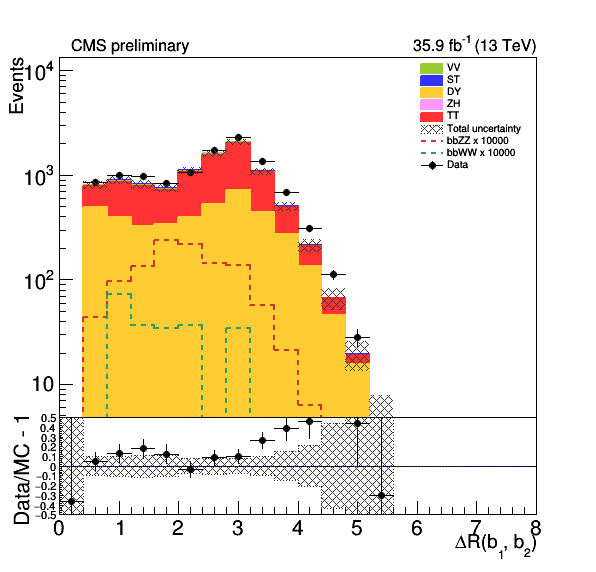
\includegraphics[width=0.43\textwidth]{figures/mm_300_april18/dR_bjets_mm_CRDY_prefit_plot_apr18.png}
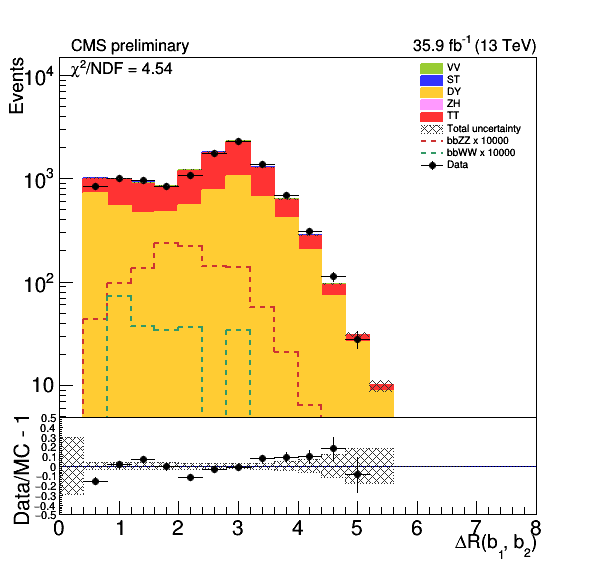
\includegraphics[width=0.43\textwidth]{figures/mm_300_april18/dR_bjets_mm_CRDY_FullPostfit_plot_apr18.png}\\
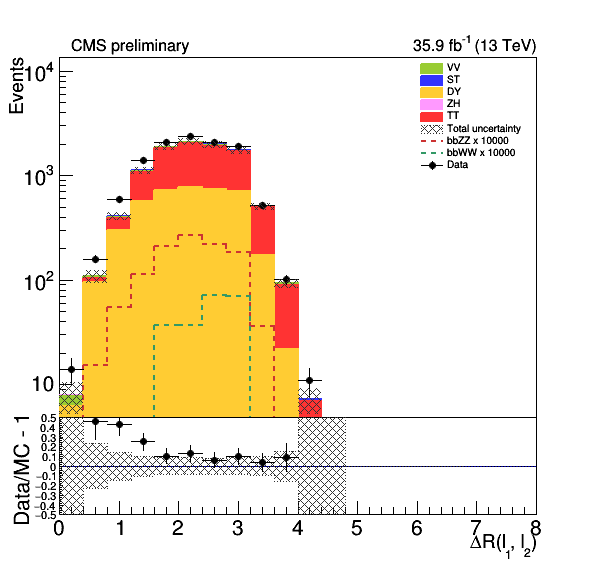
\includegraphics[width=0.43\textwidth]{figures/mm_300_april18/dR_leps_mm_CRDY_prefit_plot_apr18.png}
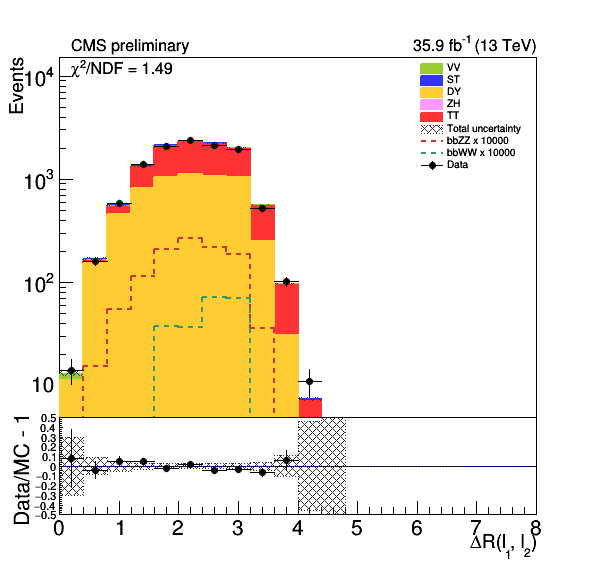
\includegraphics[width=0.43\textwidth]{figures/mm_300_april18/dR_leps_mm_CRDY_FullPostfit_plot_apr18.png}\\
% 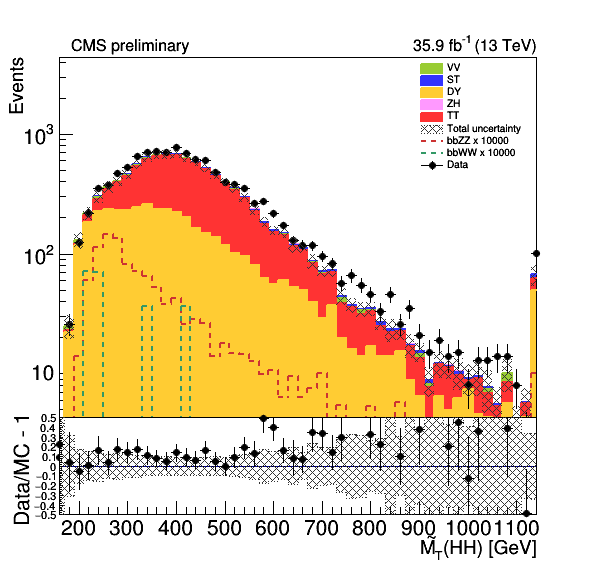
\includegraphics[width=0.31\textwidth]{figures/mm_300_april18/hhMt_mm_CRDY_prefit_plot_apr18.png}
% 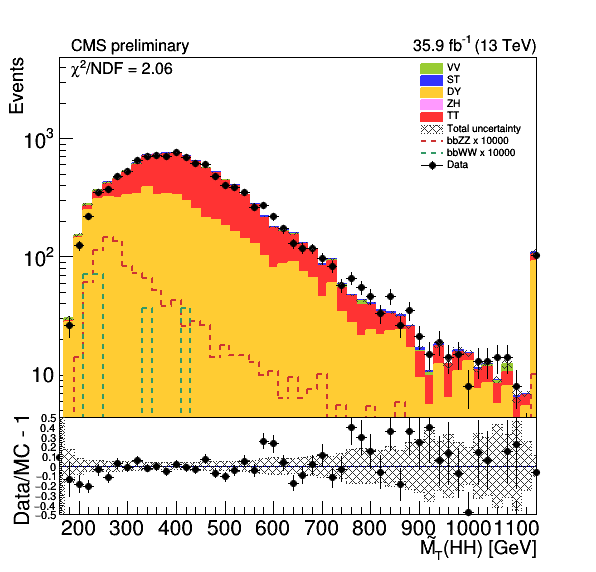
\includegraphics[width=0.31\textwidth]{figures/mm_300_april18/hhMt_mm_CRDY_FullPostfit_plot_apr18.png}\\
\caption[Data-MC comparison in CRDY.]{Comparison of data and MC samples. 300 GeV graviton mass hypothesis, CRDY region, $\mu\mu$ channel. Pre-fit plot on the left; Post-fit plot on the right.}
\label{MCcomparisons_mm_low_CRDY_1}
\end{center}
\end{figure}


\begin{figure}[H]
\begin{center}
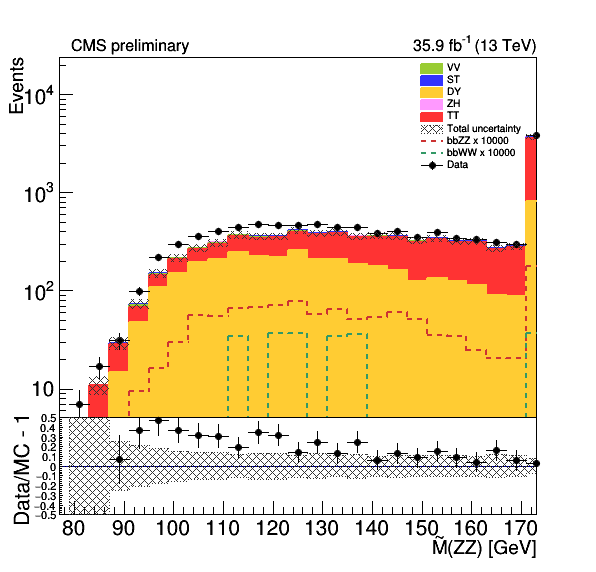
\includegraphics[width=0.43\textwidth]{figures/mm_300_april18/hmass0_mm_CRDY_prefit_plot_apr18.png}
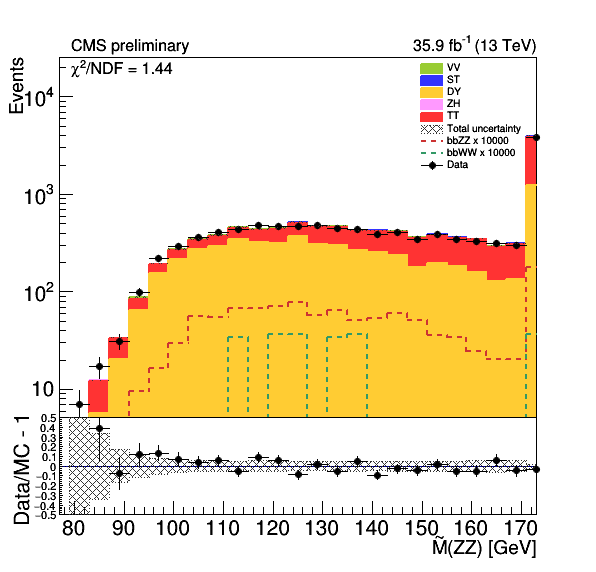
\includegraphics[width=0.43\textwidth]{figures/mm_300_april18/hmass0_mm_CRDY_FullPostfit_plot_apr18.png}\\
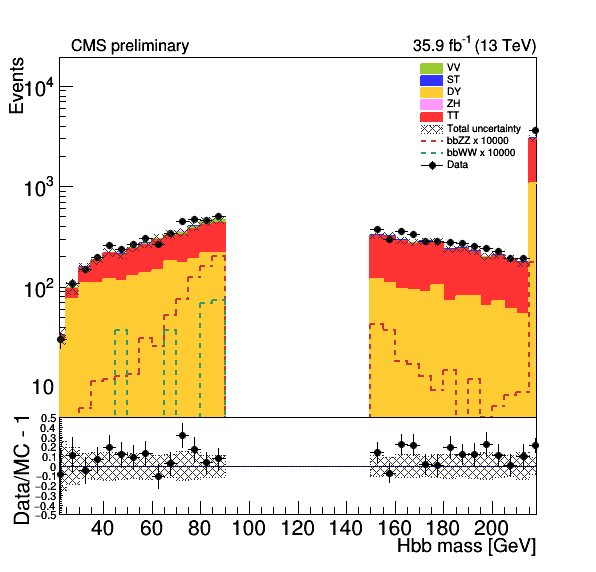
\includegraphics[width=0.43\textwidth]{figures/mm_300_april18/hmass1_mm_CRDY_prefit_plot_apr18.png}
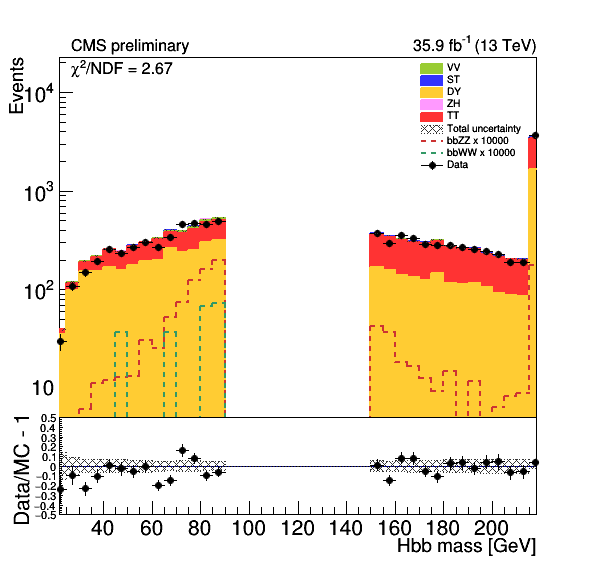
\includegraphics[width=0.43\textwidth]{figures/mm_300_april18/hmass1_mm_CRDY_FullPostfit_plot_apr18.png}\\
\caption[Data-MC comparison in CRDY.]{Comparison of data and MC samples. 300 GeV graviton mass hypothesis, CRDY region, $\mu\mu$ channel. Pre-fit plot on the left; Post-fit plot on the right.}
\label{MCcomparisons_mm_low_CRDY_2}
\end{center}
\end{figure}

\begin{figure}[H]
\begin{center}
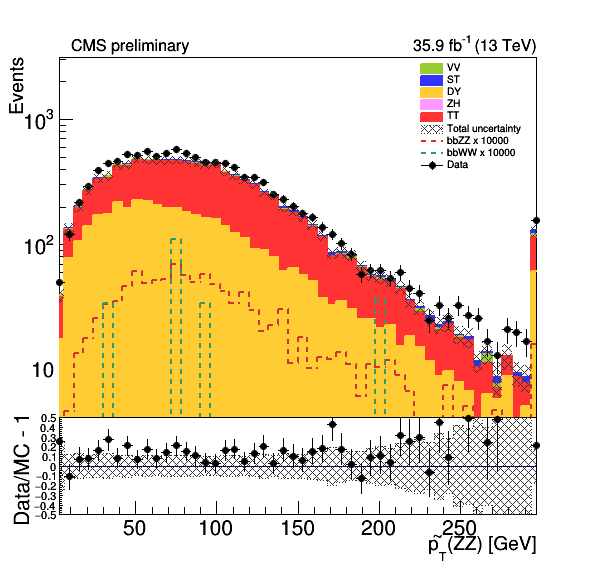
\includegraphics[width=0.43\textwidth]{figures/mm_300_april18/hpt0_mm_CRDY_prefit_plot_apr18.png}
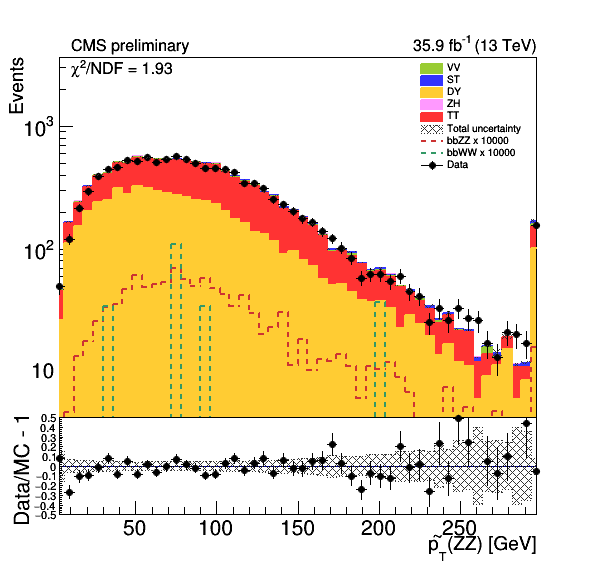
\includegraphics[width=0.43\textwidth]{figures/mm_300_april18/hpt0_mm_CRDY_FullPostfit_plot_apr18.png}\\
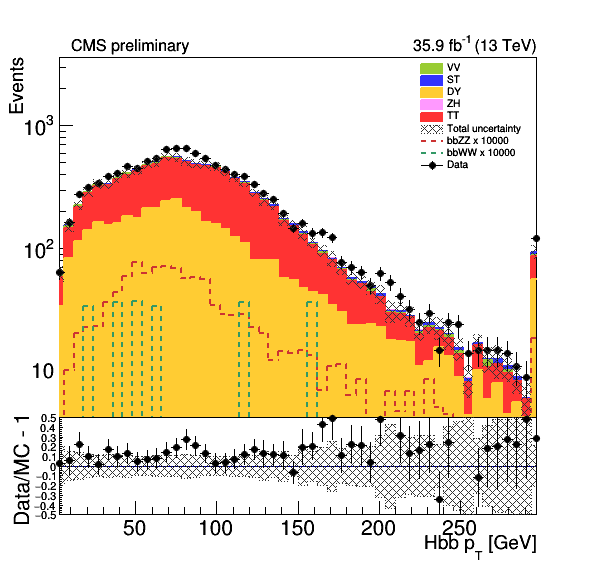
\includegraphics[width=0.43\textwidth]{figures/mm_300_april18/hpt1_mm_CRDY_prefit_plot_apr18.png}
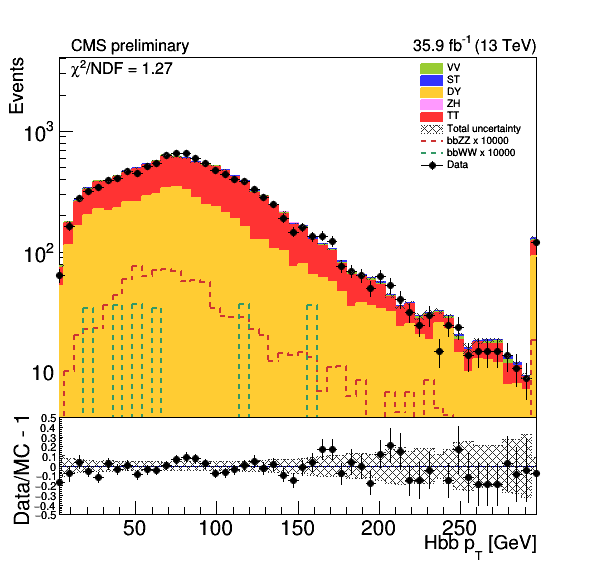
\includegraphics[width=0.43\textwidth]{figures/mm_300_april18/hpt1_mm_CRDY_FullPostfit_plot_apr18.png}\\
\caption[Data-MC comparison in CRDY.]{Comparison of data and MC samples. 300 GeV graviton mass hypothesis, CRDY region, $\mu\mu$ channel. Pre-fit plot on the left; Post-fit plot on the right.}
\label{MCcomparisons_mm_low_CRDY_3}
\end{center}
\end{figure}

\begin{figure}[H]
\begin{center}
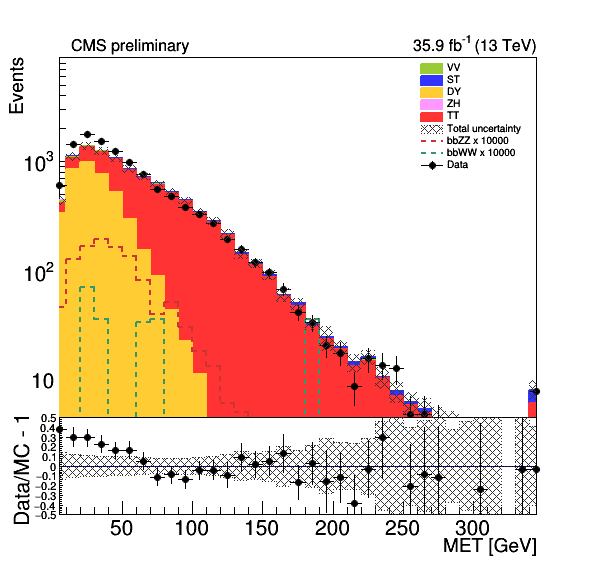
\includegraphics[width=0.43\textwidth]{figures/mm_300_april18/met_pt_mm_CRDY_prefit_plot_apr18.png}
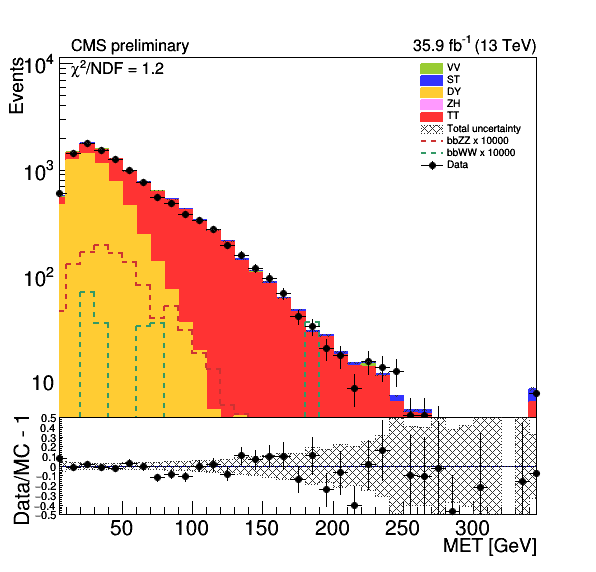
\includegraphics[width=0.43\textwidth]{figures/mm_300_april18/met_pt_mm_CRDY_FullPostfit_plot_apr18.png}\\
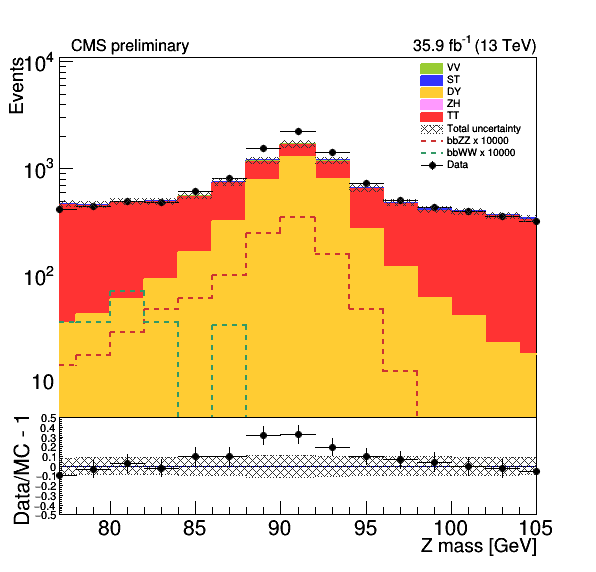
\includegraphics[width=0.43\textwidth]{figures/mm_300_april18/zmass_mm_CRDY_prefit_plot_apr21.png}
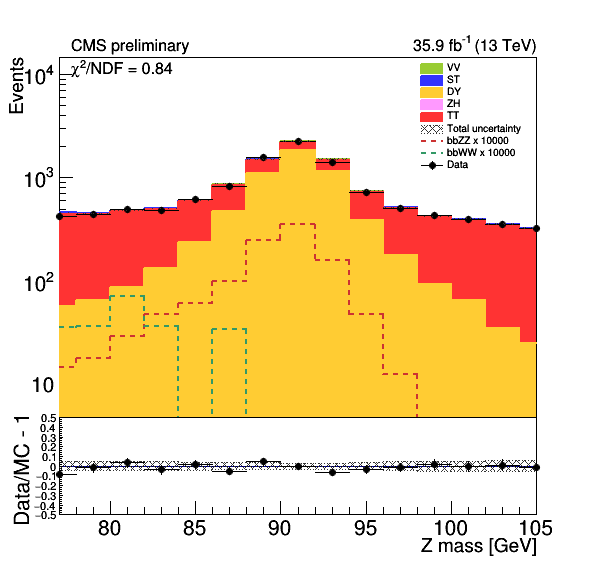
\includegraphics[width=0.43\textwidth]{figures/mm_300_april18/zmass_mm_CRDY_FullPostfit_plot_apr21.png}\\
\caption[Data-MC comparison in CRDY.]{Comparison of data and MC samples. 300 GeV graviton mass hypothesis, CRDY region, $\mu\mu$ channel. Pre-fit plot on the left; Post-fit plot on the right.}
\label{MCcomparisons_mm_low_CRDY_4}
\end{center}
\end{figure}

% 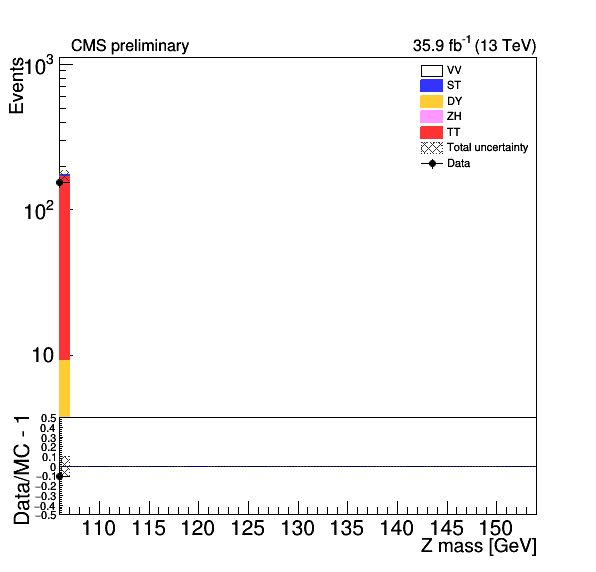
\includegraphics[width=0.31\textwidth]{figures/mm_300_april18/zmass_high_mm_CRDY_prefit_plot_apr18.png} 
% 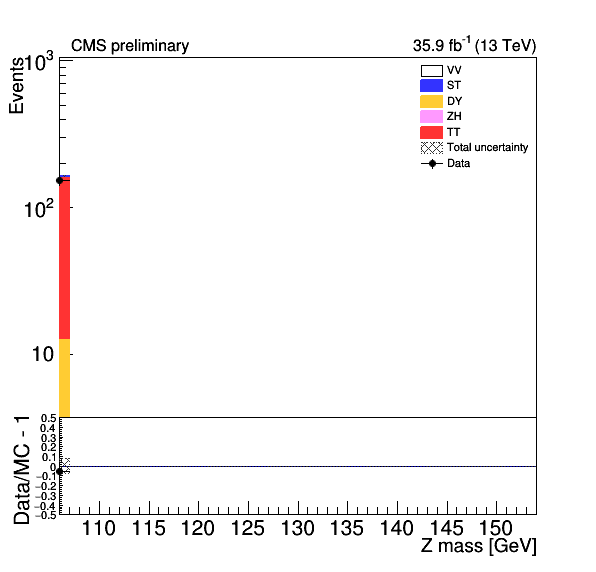
\includegraphics[width=0.31\textwidth]{figures/mm_300_april18/zmass_high_mm_CRDY_FullPostfit_plot_apr18.png}\\ 
\begin{figure}[H]
\begin{center}
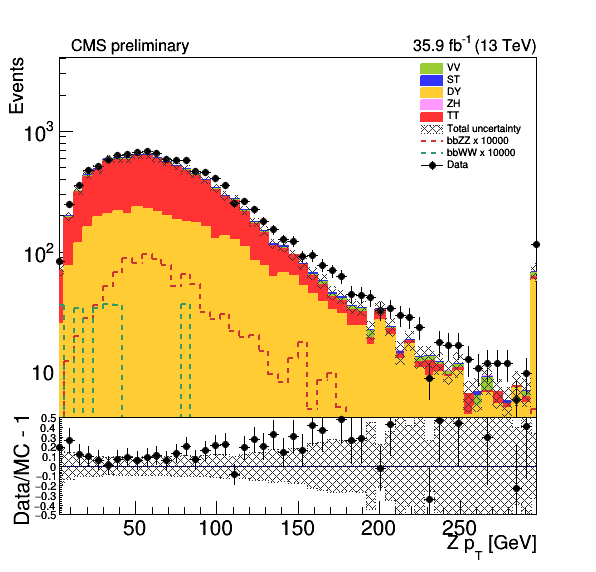
\includegraphics[width=0.43\textwidth]{figures/mm_300_april18/zpt0_mm_CRDY_prefit_plot_apr18.png}
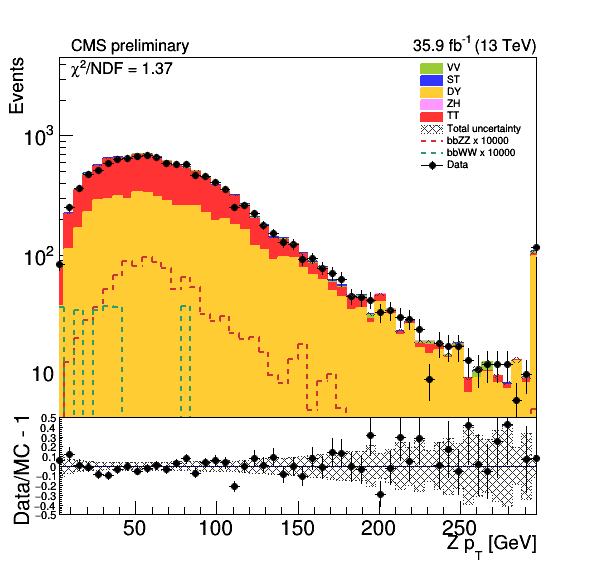
\includegraphics[width=0.43\textwidth]{figures/mm_300_april18/zpt0_mm_CRDY_FullPostfit_plot_apr18.png}\\
\caption[Data-MC comparison in CRDY.]{Comparison of data and MC samples. 300 GeV graviton mass hypothesis, CRDY region, $\mu\mu$ channel. Pre-fit plot on the left; Post-fit plot on the right.}
\label{MCcomparisons_mm_low_CRDY_5}
\end{center}
\end{figure}


%~~~~~~~~~~~~~~~~~~~~~~~~~~~~~~~~~~~~~~~~~~~~~~~~~~~~~~~~~~~~~~~~~~~~~~~~~~~~~~~~~~~~~~~~~~~~~~~~~~~~                                                                                                             

\begin{figure}[H]
  \begin{center}
    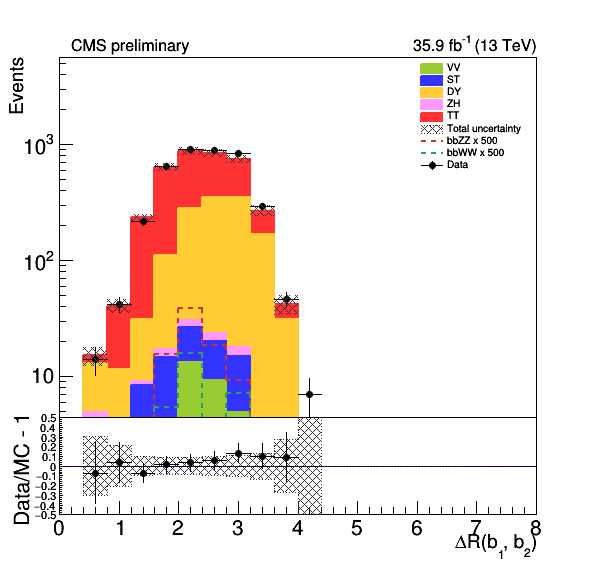
\includegraphics[width=0.43\textwidth]{figures/mm_300_april18/mm_300_good_SR_bdt_sideBand_april18/dR_bjets_mm_SR_prefit_plot_apr18.png}
    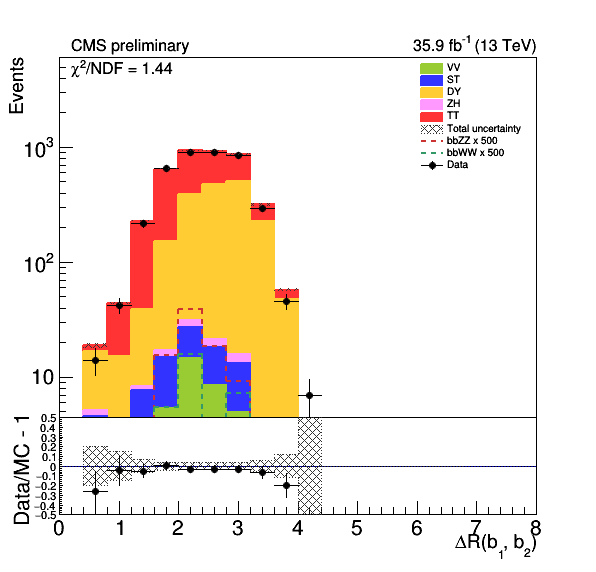
\includegraphics[width=0.43\textwidth]{figures/mm_300_april18/mm_300_good_SR_bdt_sideBand_april18/dR_bjets_mm_SR_FullPostfit_plot_apr18.png}\\
    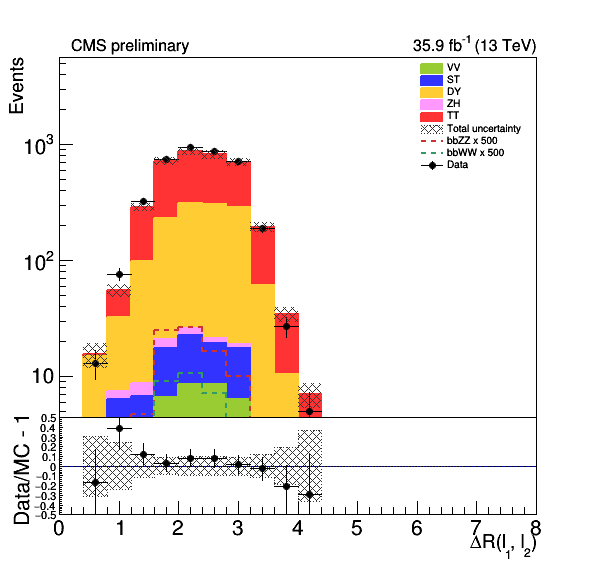
\includegraphics[width=0.43\textwidth]{figures/mm_300_april18/mm_300_good_SR_bdt_sideBand_april18/dR_leps_mm_SR_prefit_plot_apr18.png}
    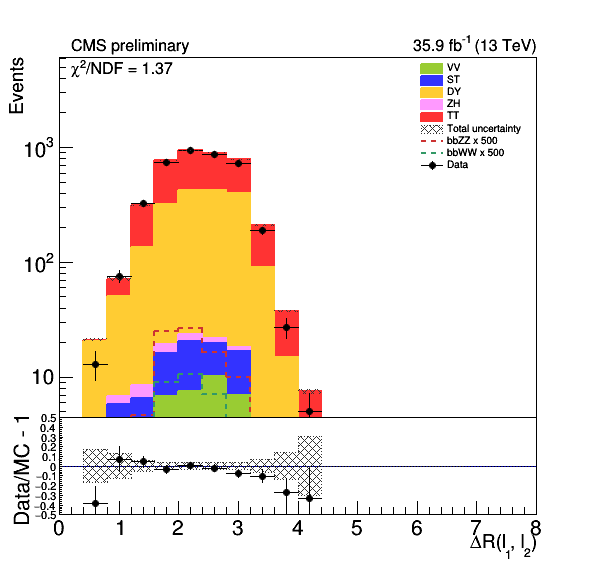
\includegraphics[width=0.43\textwidth]{figures/mm_300_april18/mm_300_good_SR_bdt_sideBand_april18/dR_leps_mm_SR_FullPostfit_plot_apr18.png}\\
%    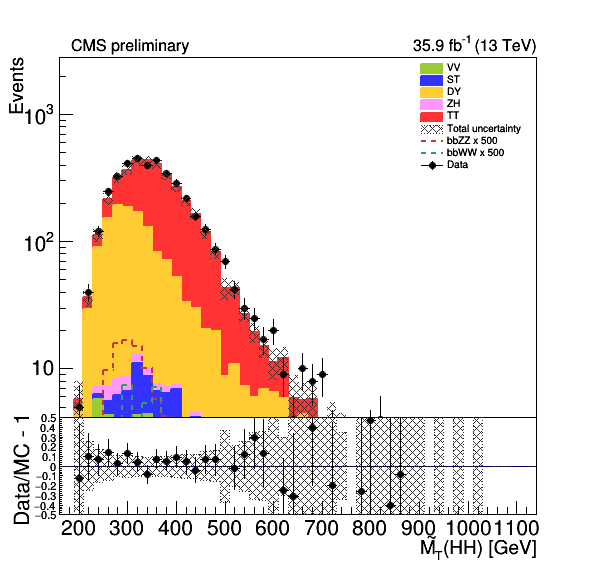
\includegraphics[width=0.31\textwidth]{figures/mm_300_april18/mm_300_good_SR_bdt_sideBand_april18/hhMt_mm_SR_prefit_plot_apr18.png}
%    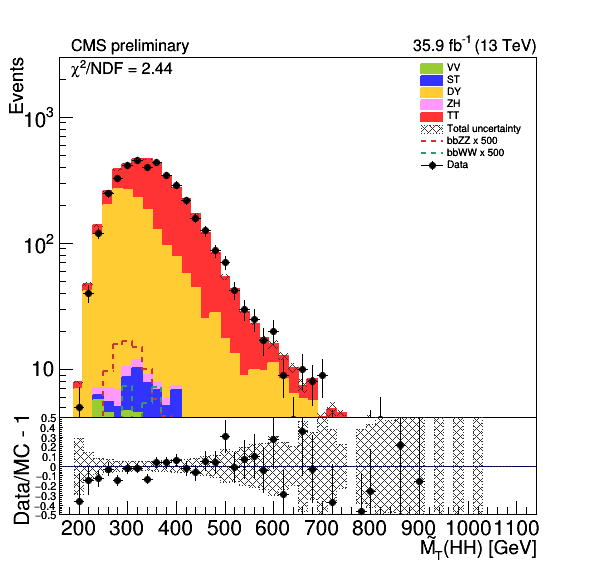
\includegraphics[width=0.31\textwidth]{figures/mm_300_april18/mm_300_good_SR_bdt_sideBand_april18/hhMt_mm_SR_FullPostfit_plot_apr18.png}\\
\caption[Data-MC comparison in the BDT sideband of the SR.]{Comparison of data and MC samples. 300 GeV graviton mass hypothesis, BDT sideband of the SR, $\mu\mu$ channel. Pre-fit plot on the left; Post-fit plot on the right.}
    \label{MCcomparisons_mm_low_SR_bdt_sideband_1}
  \end{center}
\end{figure}


\begin{figure}[H]
  \begin{center}
    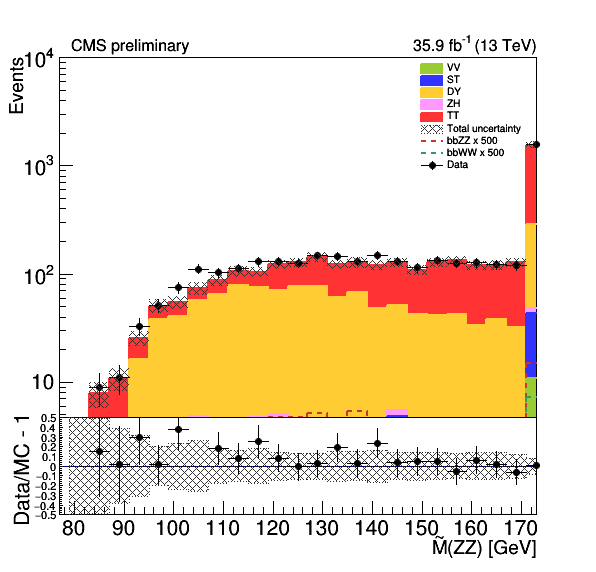
\includegraphics[width=0.43\textwidth]{figures/mm_300_april18/mm_300_good_SR_bdt_sideBand_april18/hmass0_mm_SR_prefit_plot_apr18.png}
    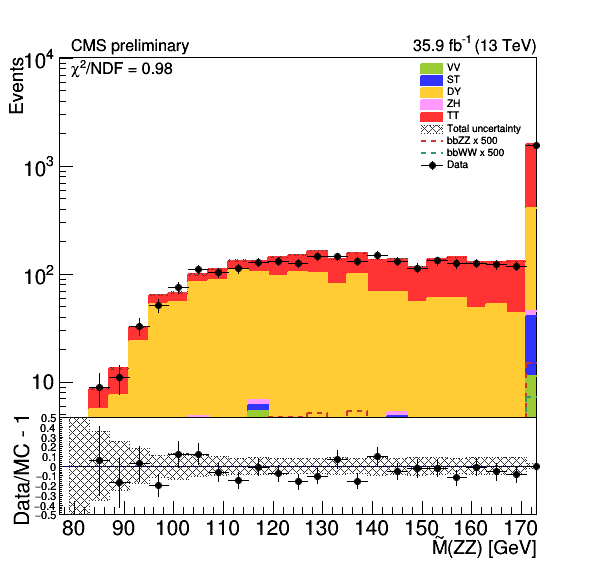
\includegraphics[width=0.43\textwidth]{figures/mm_300_april18/mm_300_good_SR_bdt_sideBand_april18/hmass0_mm_SR_FullPostfit_plot_apr18.png}\\
    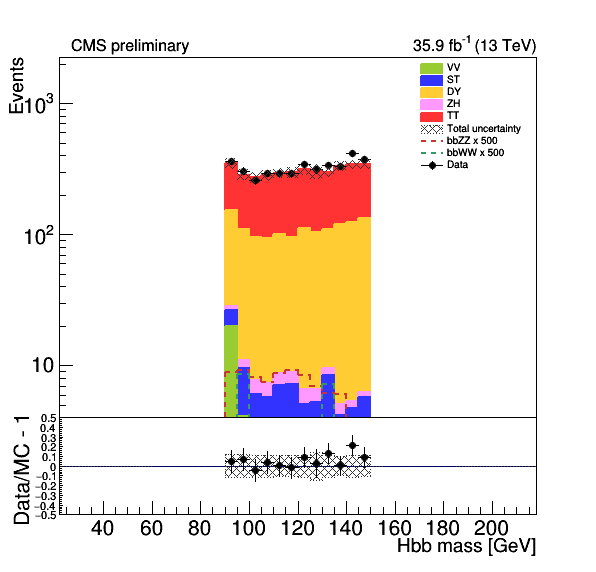
\includegraphics[width=0.43\textwidth]{figures/mm_300_april18/mm_300_good_SR_bdt_sideBand_april18/hmass1_mm_SR_prefit_plot_apr18.png}
    \includegraphics[width=0.43\textwidth]{figures/mm_300_april18/mm_300_good_SR_bdt_sideBand_april18/hmass1_mm_SR_FullPostfit_plot_apr18.png}\\
\caption[Data-MC comparison in the BDT sideband of the SR.]{Comparison of data and MC samples. 300 GeV graviton mass hypothesis, BDT sideband of the SR, $\mu\mu$ channel. Pre-fit plot on the left; Post-fit plot on the right.}
    \label{MCcomparisons_mm_low_SR_bdt_sideband_2}
  \end{center}
\end{figure}

\begin{figure}[H]
  \begin{center}
    \includegraphics[width=0.43\textwidth]{figures/mm_300_april18/mm_300_good_SR_bdt_sideBand_april18/hpt0_mm_SR_prefit_plot_apr18.png}
    \includegraphics[width=0.43\textwidth]{figures/mm_300_april18/mm_300_good_SR_bdt_sideBand_april18/hpt0_mm_SR_FullPostfit_plot_apr18.png}\\
    \includegraphics[width=0.43\textwidth]{figures/mm_300_april18/mm_300_good_SR_bdt_sideBand_april18/hpt1_mm_SR_prefit_plot_apr18.png}
    \includegraphics[width=0.43\textwidth]{figures/mm_300_april18/mm_300_good_SR_bdt_sideBand_april18/hpt1_mm_SR_FullPostfit_plot_apr18.png}\\
    \caption[Data-MC comparison in the BDT sideband of the SR.]{Comparison of data and MC samples. 300 GeV graviton mass hypothesis, BDT sideband of the SR, $\mu\mu$ channel. Pre-fit plot on the left; Post-fit plot on the right.}
    \label{MCcomparisons_mm_low_SR_bdt_sideband_3}
  \end{center}
\end{figure}

    \begin{figure}[H]
  \begin{center}
    \includegraphics[width=0.43\textwidth]{figures/mm_300_april18/mm_300_good_SR_bdt_sideBand_april18/met_pt_mm_SR_prefit_plot_apr18.png}
    \includegraphics[width=0.43\textwidth]{figures/mm_300_april18/mm_300_good_SR_bdt_sideBand_april18/met_pt_mm_SR_FullPostfit_plot_apr18.png}\\
%    \includegraphics[width=0.31\textwidth]{figures/mm_300_april18/mm_300_good_SR_bdt_sideBand_april18/zmass_high_mm_SR_prefit_plot_apr18.png}
 %   \includegraphics[width=0.31\textwidth]{figures/mm_300_april18/mm_300_good_SR_bdt_sideBand_april18/zmass_high_mm_SR_FullPostfit_plot_apr18.png}\\
    \includegraphics[width=0.43\textwidth]{figures/mm_300_april18/mm_300_good_SR_bdt_sideBand_april18/zpt0_mm_SR_prefit_plot_apr18.png}
    \includegraphics[width=0.43\textwidth]{figures/mm_300_april18/mm_300_good_SR_bdt_sideBand_april18/zpt0_mm_SR_FullPostfit_plot_apr18.png}\\
\caption[Data-MC comparison in the BDT sideband of the SR.]{Comparison of data and MC samples. 300 GeV graviton mass hypothesis, BDT sideband of the SR, $\mu\mu$ channel. Pre-fit plot on the left; Post-fit plot on the right.}
    \label{MCcomparisons_mm_low_SR_bdt_sideband_4}
  \end{center}
\end{figure}



%~~~~~~~~~~~~~~~~~~~~~~~~~~~~~~~~~~~~~~~~~~~~~~~~~~~~~~~~~~~~~~~~~~~~~~~~~~~~~~~~~~~~~~~~~~~~~~~~~~~~ 
\begin{figure}[H]
\begin{center}
\includegraphics[width=0.43\textwidth]{figures/mm_300_april18/dR_bjets_mm_CRTT_prefit_plot_apr18.png}
\includegraphics[width=0.43\textwidth]{figures/mm_300_april18/dR_bjets_mm_CRTT_FullPostfit_plot_apr18.png}\\
\includegraphics[width=0.43\textwidth]{figures/mm_300_april18/dR_leps_mm_CRTT_prefit_plot_apr18.png}
\includegraphics[width=0.43\textwidth]{figures/mm_300_april18/dR_leps_mm_CRTT_FullPostfit_plot_apr18.png}\\
% \includegraphics[width=0.31\textwidth]{figures/mm_300_april18/hhMt_mm_CRTT_prefit_plot_apr18.png}
%\includegraphics[width=0.31\textwidth]{figures/mm_300_april18/hhMt_mm_CRTT_FullPostfit_plot_apr18.png}\\
\caption[Data-MC comparison in CRTT.]{Comparison of data and MC samples. 300 GeV graviton mass hypothesis, CRTT region, $\mu\mu$ channel. Pre-fit plot on the left; Post-fit plot on the right.}
\label{MCcomparisons_mm_low_CRTT_1}
\end{center}
\end{figure}


\begin{figure}[H]
\begin{center}
\includegraphics[width=0.43\textwidth]{figures/mm_300_april18/hmass0_mm_CRTT_prefit_plot_apr18.png}
\includegraphics[width=0.43\textwidth]{figures/mm_300_april18/hmass0_mm_CRTT_FullPostfit_plot_apr18.png}\\
\includegraphics[width=0.43\textwidth]{figures/mm_300_april18/hmass1_mm_CRTT_prefit_plot_apr18.png}
\includegraphics[width=0.43\textwidth]{figures/mm_300_april18/hmass1_mm_CRTT_FullPostfit_plot_apr18.png}\\
\caption[Data-MC comparison in CRTT.]{Comparison of data and MC samples. 300 GeV graviton mass hypothesis, CRTT region, $\mu\mu$ channel. Pre-fit plot on the left; Post-fit plot on the right.}
\label{MCcomparisons_mm_low_CRTT_2}
\end{center}
\end{figure}

\begin{figure}[H]
\begin{center}
\includegraphics[width=0.43\textwidth]{figures/mm_300_april18/hpt0_mm_CRTT_prefit_plot_apr18.png}
\includegraphics[width=0.43\textwidth]{figures/mm_300_april18/hpt0_mm_CRTT_FullPostfit_plot_apr18.png}\\
\includegraphics[width=0.43\textwidth]{figures/mm_300_april18/hpt1_mm_CRTT_prefit_plot_apr18.png}
\includegraphics[width=0.43\textwidth]{figures/mm_300_april18/hpt1_mm_CRTT_FullPostfit_plot_apr18.png}\\
\caption[Data-MC comparison in CRTT.]{Comparison of data and MC samples. 300 GeV graviton mass hypothesis, CRTT region, $\mu\mu$ channel. Pre-fit plot on the left; Post-fit plot on the right.}
\label{MCcomparisons_mm_low_CRTT_3}
\end{center}
\end{figure}


\begin{figure}[H]
\begin{center}
\includegraphics[width=0.43\textwidth]{figures/mm_300_april18/met_pt_mm_CRTT_prefit_plot_apr18.png}
\includegraphics[width=0.43\textwidth]{figures/mm_300_april18/met_pt_mm_CRTT_FullPostfit_plot_apr18.png}\\
\includegraphics[width=0.43\textwidth]{figures/mm_300_april18/zmass_high_mm_CRTT_prefit_plot_apr18.png}
\includegraphics[width=0.43\textwidth]{figures/mm_300_april18/zmass_high_mm_CRTT_FullPostfit_plot_apr18.png}\\
\caption[Data-MC comparison in CRTT.]{Comparison of data and MC samples. 300 GeV graviton mass hypothesis, CRTT region, $\mu\mu$ channel. Pre-fit plot on the left; Post-fit plot on the right.}
\label{MCcomparisons_mm_low_CRTT_4}
\end{center}
\end{figure}


\begin{figure}[H]
\begin{center}
\includegraphics[width=0.43\textwidth]{figures/mm_300_april18/zpt0_mm_CRTT_prefit_plot_apr18.png}
\includegraphics[width=0.43\textwidth]{figures/mm_300_april18/zpt0_mm_CRTT_FullPostfit_plot_apr18.png}\\
\caption[Data-MC comparison in CRTT.]{Comparison of data and MC samples. 300 GeV graviton mass hypothesis, CRTT region, $\mu\mu$ channel. Pre-fit plot on the left; Post-fit plot on the right.}
\label{MCcomparisons_mm_low_CRTT_5}
\end{center}
\end{figure}

\subsection{Multivariate discriminant: a BDT classifier}

In many areas of HEP, such as object identification, a reduction of the background contribution in the signal region, etc., there are needs to discriminate a ``signal'' from one or several ``backgrounds.'' The discriminating algorithms can use a single physical variable for signal-background separation, or several variables. The Higgs boson discovery, in part, was possible due to an employed BDT approach, where several variables are combined into an artificial BDT score or output. The BDT output, as a higher-level construct, has no direct physical interpretation. However, due to the demostrated gain in signal-background separation performance, the BDT has been successfully used for years for the final classification decision. 

Multivariate discriminants (or models or classifiers) based on the BDT or other algorithms are constructed using machine learning (ML) techniques. Now, at almost every stage of the HEP data analysis, starting from the physics object reconstruction, through the object identification and the signal region purification, and up to the construction of the final discriminating MVA variable, physicists rely on the ML methods.

In simple terms, the ML procedure consists of training and testing stages, and sometimes a validation stage is added. First, the input data are split into two non-overlapping sets: train and test data. Then the classifier is trained when the model is learning the patterns in the train data. After that, the performance of the model is tested using independent test data. 

After the training procedure, the ML algorithm produces a discriminant, which is a function that is related to the likelihood of an event to belong to a signal or to a background category. Here and in other parts of the thesis, we are describing the BDT procedure, which is a non-parametric supervised learning method used for classification; other MVA methods that are not related to this measurement, are well-explained in \cite{book:411471}. 

One prefers a classifier with low bias and low variance. A bias is the difference between the average prediction of our model and the correct value, the latter of which we are trying to predict. A classifier with a high bias oversimplifies the model and does not take into account all the nuances of a given train dataset. Therefore, analysts prefer low bias models, which are flexible and perform well both on the train and test data, and always provide a stable separation between the signal and background hypotheses. A variance is the variability of model prediction for a given data point and is related to the spread of our data (a sharp peak vs a broad distribution). A model with high variance learns almost every single pattern in the train data and, therefore, will not generalize well when given new unseen data. As a result, models with a high variance achieve the best scores using the train data but perform poorly on the test data. Thus, low variance models, which are robust when applying the trained classifiers on a dataset that is statistically independent from the one used for training, are preferable.

One of the most popular ML algorithms in HEP is based on boosted decision trees (BDT). A single decision tree is a sequence of simple binary splits on each of the input variables. The tree can thus be depicted as a multidimensional set of selections on input space. The tree assigns a score of +1 or -1 if a given event is signal or background-like. The key elements in each step of the BDT splits are the variables used for the selection and the positions of the selections. Both are determined using an impurity criterion $I(p_n)$, which is a function of the signal purity $p_n$ in a tree node $n$. As a definition of the impurity criterion for this measurement, the Gini coefficient is used: $I_G(p_n) = 2 p_n \cdot (1 - p_n)$. The signal purity is defined as a ratio of the signal contribution to the total number of signal and background events, $p_n = S/(S+B)$. The impurity criterion is chosen such that it is at the minimum when $p_n$=0 or $p_n$=1. These values would give perfect signal-background discrimination. The criterion is at the maximum, when $p_n$=0.5, which means no discrimination is achieved. 
Each split maximises the gain function $G=I(p_n) - f_1I(p_{c1})-f_2I(p_{c2})$ . In this formulation of $G$, the labels c1 and c2 refer to child nodes of the parent node, and $f_1$ and $f_2$ are the fractions of events of the parent node that are found in child nodes c1 and c2, respectively. 
The tree keeps applying the selection on the input variables until either a maximum depth is reached (a number of consecutive splits), or a minimum number of events in the final child nodes are attained. The problem with such a tree growing procedure is that it is prone to overtraining, which means the model will not generalize well and have a high variance. 

One way to deal with BDT overtraining is boosting. The idea behind boosting is that signal events from the training sample that end up in a background node or vice versa are given intentionally large weights (a penalty). These weights are normally significantly larger than the weights for events with the correct leaf node prediction. Such a penalty procedure re-weighs the train data and then new decision trees are created. The boosting is applied hundreds of times, which produces a set of new reweighted trees (a forest). Intuitively, boosting is a method in which a large number of shallow trees, which have only a few splits, are combined by taking a weighted average of their output scores. The discriminating power of a single shallow tree is usually poor, but such a tree is less prone to overtraining, therefore when combined, the ensemble of these trees produces a model with high and stable performance.

For the boosting algorithm, we chose the gradient boosting method, as is implemented in the popular MVA package for HEP - TMVA \cite{Hocker:2007ht}. Gradient boosting can be thought of as a function expansion approach. In this case, each tree corresponds to a summand. In this approach, the parameters for each summand (tree) are determined by minimizing an error function. In the TMVA implementation, the binomial log-likelihood loss function is used. The adopted procedure follows the greedy algorithm approach - only one tree is modified at a time, while the other trees remain invariable.

Several decision trees of the BDT procedure which were employed in the analysis are shown below. This training was done in the di-electron channel. In all figures produced by TMVA, index 0 refers to \HZZ~candidate and index 1 refers to \HBB~candidate. For example, ``hmass1'' denotes the mass of the \HZZ~candidate, ``hpt0'' denotes the $p_T$ of the \HBB~candidate, etc. For the Z boson candidate, the on-shell Z boson decaying to charged leptons, \Zll, has either an index 0 or the index is dropped. The closer the node color is to blue, the more the event is classified as signal-like.The same idea is illustrated with the red color for background events. \label{TMVA_notation}

Di-electron and di-muon channels have been trained separately and the BDT metrics (discussed later in this chapter) show similar performance. To save space, in this chapter we show mostly figures related to the di-electron channel.

\begin{figure}[H]
\begin{center}
\includegraphics[width=0.94\textwidth]{BDT_0.pdf}
\includegraphics[width=0.94\textwidth]{BDT_1.pdf}\\
\caption[BDT trees 1 and 2.]{BDT trees 1 and 2 (indexing starts from 0). These trees relied on: the mass and the $p_T$ of the \Zll~candidate, $\Delta R$ separation between two b jets, the mass of the \HBB~candidate, and the $p_T$ of the $ZZ^*$ system. The TMVA notation is explained in \ref{TMVA_notation}.}
\label{fig:bdt_trees}
\end{center}
\end{figure}

\begin{figure}[H]
\begin{center}
\includegraphics[width=0.94\textwidth]{BDT_399.pdf}
\includegraphics[width=0.94\textwidth]{BDT_400.pdf}\\
\caption[BDT trees 400 and 401.]{BDT trees 400 and 401 (indexing starts from 0). These trees relied on: the $p_T$ of the \Zll~candidate, 
$\Delta R$ separation between two b jets,
$\Delta R$ separation between two charged leptons, 
the $p_T$ of the \HBB~candidate, and the mass and the $p_T$ of the $ZZ^*$ system. The TMVA notation is explained in \ref{TMVA_notation}.} 
\label{fig:bdt_trees_2}
\end{center}
\end{figure}

\begin{figure}[H]
\begin{center}
\includegraphics[width=0.94\textwidth]{BDT_798.pdf}
\includegraphics[width=0.94\textwidth]{BDT_799.pdf}\\
\caption[BDT trees 799 and 800.]{BDT trees 799 and 800 (indexing starts from 0). These trees relied on: the $p_T$ of the \Zll~candidate, 
$\Delta R$ separation between two b jets,
$\Delta R$ separation between two charged leptons, 
the mass of the \HBB~candidate, and the mass of the $ZZ^*$ system. The TMVA notation is explained in \ref{TMVA_notation}.} 
\label{fig:bdt_trees_3}
\end{center}
\end{figure}

The BDT discriminant is trained on a pure sample of signal and background events from simulation, using the train data. The properties of the discriminant are studied on an independent testing sample of pure signal and background events, using the test data. The Deep Neural Network (DNN) approach has also been studied - however, due to the lack of event statistics, the DNN approach could not offer a performance higher than the one achieved with the BDT, and thus was abandoned. Training 16 BDTs per spin hypothesis seemed impractical since our data analysis is dominated by statistical uncertainties. Instead, we follow the approach of other $HH$ analyses \cite{HH_combination}: we split the range from 250 to 1000 into two regions: low mass (250 to 450 GeV) and high mass (above 450 GeV up to 1 TeV) regions. This separation boundary at 450 GeV was optimized first using ROC curves (described later in this section), then by running the whole analysis chain all the way to the final limits. %This procedure not only saves CPU cycles by training two BDTs instead of sixteen, but mostly increases the statistics and improves the robustness of the trained BDT. 

During the training procedure some variables provide more discriminating power and on average are used more often than others. The more often the variable is used, the higher its importance is. The tables below show the ranking and average importance of each of the BDT training. For the low and high mass regions, and di-electron and di-muon channels, see Tables \ref{tab:importance_ee_low}, \ref{tab:importance_ee_high}, \ref{tab:importance_mm_low}, \ref{tab:importance_mm_high}. As can be seen from these Tables, all nine selected variables are equally important, and one cannot use 1-2 single variables to perform signal-background discrimination. The ranking of variables is compatible between di-electron and di-muon channels within the statistical uncertainty of $O$(sub percent), the graviton signal hypothesis is shown. 

\noindent\begin{table}[H]
\centering
\begin{tabular}{|c| l |c|}\hline
Rank & Variable & Importance (\%) \\\hline
1 & $\Delta R_{b\ jets}$ & 13.9 \\ 
2 & MET & 12.1 \\ 
3 & Mass of $\HBB$~candidate & 11.9 \\ 
4 & $p_T^{ZZ^*}$ & 11.0 \\ 
5 & $\Delta R_{leptons}$ & 10.9 \\ 
6 & $p_T$ of $\HBB$~candidate & 10.7 \\ 
7 & $p_T$ of Z boson candidate & 10.2 \\ 
8 & Mass of $ZZ^*$ system & 10.1 \\ 
9 & Mass of Z boson candidate & 9.26 \\ 
\hline
\end{tabular}
\captionof{table}{Di-electron channel. Relative importance of the input variables in the low mass BDT training.}
\label{tab:importance_ee_low}
\end{table}
\begin{table}
\centering
\begin{tabular}{|c| l |c|}\hline
Rank & Variable & Importance (\%) \\\hline
1 & $\Delta R_{leptons}$ & 14.1 \\ 
2 & Mass of $\HBB$~candidate & 13.7 \\ 
3 & $\Delta R_{b\ jets}$ & 13.2 \\ 
4 & $p_T$ of $\HBB$~candidate & 12.1 \\ 
5 & $p_T$ of Z boson candidate & 11.5 \\ 
6 & $p_T^{ZZ^*}$ & 11.3 \\ 
7 & MET & 10.3 \\ 
8 & Mass of $ZZ^*$ system & 7.7 \\ 
9 & Mass of Z boson candidate & 6.1 \\ 
\hline
\end{tabular}
\captionof{table}{Di-electron channel. Relative importance of the input variables in the high mass BDT training.}
\label{tab:importance_ee_high}
\end{table}

\vspace{2cm}
%%%%%%%%%%%%%%%%%%%%%%%%
%%%%%%%%%%%%%%%%%%%%%%%%
\noindent\begin{table}[H]
\centering
\begin{tabular}{|c| l |c|}\hline
Rank & Variable & Importance (\%) \\\hline
1 & $\Delta R_{b\ jets}$ & 13.0 \\ 
2 & MET & 12.2 \\ 
3 & Mass of $\HBB$~candidate & 11.9 \\ 
4 & $p_T$ of $\HBB$~candidate & 11.3 \\ 
5 & $p_T$ of Z boson candidate & 11.1 \\ 
6 & $p_T^{ZZ^*}$ & 10.9 \\ 
7 & $\Delta R_{leptons}$ & 10.5 \\ 
8 & Mass of $ZZ^*$ system & 9.7 \\ 
9 & Mass of Z boson candidate & 9.5 \\ 
\hline
\end{tabular}
\captionof{table}{Di-muon channel. Relative importance of the input variables in the low mass BDT training.}
\label{tab:importance_mm_low}
\end{table}
\begin{table}
\centering
\begin{tabular}{|c| l |c|}\hline
Rank & Variable & Importance (\%) \\\hline
1 & Mass of $\HBB$~candidate & 13.8 \\ 
2 & $\Delta R_{b\ jets}$ & 13.1 \\ 
3 & $\Delta R_{leptons}$ & 12.9 \\ 
4 & $p_T$ of \HBB~candidate & 11.7 \\ 
5 & $p_T^{ZZ^*}$ & 11.3 \\ 
6 & $p_T$ of Z boson candidate & 11.1 \\ 
7 & MET & 11.0 \\ 
8 & Mass of $ZZ^*$ system & 8.8 \\ 
9 & Mass of Z boson candidate & 6.2 \\ 
\hline
\end{tabular}
\captionof{table}{Di-muon channel. Relative importance of the input variables in the high mass BDT training.}
\label{tab:importance_mm_high}
\end{table}

The correlations among the input variables are shown in the Figs. ~\ref{fig:ele_cors_low}, ~\ref{fig:ele_cors_high} (graviton hypothesis). For low mass training, signal samples for mass hypotheses from 250 to 450 GeV are combined together and represent the ``signal''. This is done similarly for high mass training - it is a mix of signal samples for mass hypotheses from 500 to 1000 GeV. For background samples, the ``background'' is a mix of samples of two main background processes: DY in association with jets and $t\bar{t}$ production, weighted by the cross section value. The full selection is applied except for the Z boson and \HBB~ candidate invariant mass requirements. 

\begin{figure}[tbp]
\begin{center}
\includegraphics[width=0.75\textwidth]{bdtPlots_eles/low_corS.pdf}
\includegraphics[width=0.75\textwidth]{bdtPlots_eles/low_corB.pdf}
\caption[Input variable correlations of the di-electron channel, low mass training.]{ Input variable correlations of the di-electron channel, low mass training. Top: signal sample mix. Bottom: background sample mix. The TMVA notation is explained in \ref{TMVA_notation}.}
\label{fig:ele_cors_low}
\end{center}
\end{figure}

\begin{figure}[tbp]
\begin{center}
\includegraphics[width=0.75\textwidth]{bdtPlots_eles/high_corS.pdf}
\includegraphics[width=0.75\textwidth]{bdtPlots_eles/high_corB.pdf}
\caption[Input variable correlations of the di-electron channel, high mass training.]{ Input variable correlations of the di-electron channel, high mass training. Top: signal sample mix. Bottom: background sample mix. The TMVA notation is explained in \ref{TMVA_notation}.}
\label{fig:ele_cors_high}
\end{center}
\end{figure}

Below we include figures of the BDT input variables. They are the same variables previously shown, but are produced by the TMVA package. In this style they allow for an easier visual judgment of which variables behave with greater difference between the signal and the background, see Figs. \ref{fig:ele_lowVars}, \ref{fig:ele_highVars} for the BDT training in the di-electron channel, graviton hypothesis. For the radion hypothesis, the separation power of the individual variables slightly varies, but overall the BDT training has a similar performance. The input variables to the BDT training of the radion signal hypothesis in the di-electron channel are shown in Figs. \ref{fig:ele_lowVars_radion}, \ref{fig:ele_highVars_radion}.

\begin{figure}[H]
\begin{center}
\includegraphics[width=0.95\textwidth]{bdtPlots_eles/low_vars1.pdf}
\includegraphics[width=0.95\textwidth]{bdtPlots_eles/low_vars2.pdf}
\caption[Variables used in the low mass training for di-electron channel, graviton hypothesis.]{ Variables used in the low mass training for di-electron channel, graviton hypothesis. Index '1' refers to \HBB~decay and index '0' refers to \HZZ~decay. The TMVA notation is explained in \ref{TMVA_notation}.}
\label{fig:ele_lowVars}
\end{center}
\end{figure}

\begin{figure}[H]
\begin{center}
\includegraphics[width=0.95\textwidth]{bdtPlots_eles/high_vars1.pdf}
\includegraphics[width=0.95\textwidth]{bdtPlots_eles/high_vars2.pdf}
\caption[Variables used in the high mass training for di-electron channel, graviton hypothesis.]{ Variables used in the high mass training for di-electron channel, graviton hypothesis. Index '1' refers to \HBB~decay and index '0' refers to \HZZ~decay. The TMVA notation is explained in \ref{TMVA_notation}.}
\label{fig:ele_highVars}
\end{center}
\end{figure}

%%%%%%%%%%%%%%%%%%%%%%%%%%%%%%%%%%
\begin{figure}[H]
\begin{center}
\includegraphics[width=0.95\textwidth]{radion_ee_low_bdt/radion_variables_id_c1.pdf}
\includegraphics[width=0.95\textwidth]{radion_ee_low_bdt/radion_variables_id_c2.pdf}
\caption[Variables used in the low mass training for di-electron channel, radion hypothesis.]{ Variables used in the low mass training for di-electron channel, radion hypothesis. Index '1' refers to \HBB~decay and index '0' refers to \HZZ~decay. The TMVA notation is explained in \ref{TMVA_notation}.}
\label{fig:ele_lowVars_radion}
\end{center}
\end{figure}

\begin{figure}[H]
\begin{center}
\includegraphics[width=0.95\textwidth]{radion_ee_high_bdt/radion_variables_id_c1.pdf}
\includegraphics[width=0.95\textwidth]{radion_ee_high_bdt/radion_variables_id_c2.pdf}
\caption[Variables used in the high mass training for di-electron channel, radion hypothesis.]{ Variables used in the high mass training for di-electron channel, radion hypothesis. Index '1' refers to \HBB~decay and index '0' refers to \HZZ~decay. The TMVA notation is explained in \ref{TMVA_notation}.}
\label{fig:ele_highVars_radion}
\end{center}
\end{figure}



After the training, the BDT model is created. This model produces the BDT distribution (BDT response), see Fig. \ref{fig:ele_BDTs}. This figure overlays train and test parameters of the BDT training of the di-electron channel. The parameters of the model, such as the number of trees, the allowed number of splits per variable, the maximum tree depth and others, have been thoroughly studied. The default TMVA parameters are found to provide a good performance with this measurement. 

It is difficult to get high performance during low mass training, since
in this region kinematic properties of the background processes are similar to those of the signal, see Figs. ~\ref{fig:ele_lowVars}, ~\ref{fig:ele_highVars}. The event yield of background in this region is very high and most variables have similar distributions for signal and background processes. The BDT performance is noticeably better than what can be achieved using a simple linear discriminant method (LD), see Figs. ~\ref{fig:ele_BDTs}, ~\ref{fig:ele_ROCs}.

Performance of the high mass training can be considered perfect, see Fig. ~\ref{fig:ele_highVars}. High mass resonances produce boosted Higgs bosons whose kinematical properties are different from those of the background processes. This is clearly seen in variables related to the boost, such as $\Delta R_{b\ jets}$, $\Delta R_{leptons}$, $p_T$ of $\HBB$~candidate, and $p_T$ of $\HZZ$~candidate. Therefore, for the high mass region even the linear
discriminant is performing well, see Figs. ~\ref{fig:ele_BDTs}, ~\ref{fig:ele_ROCs}.

\begin{figure}[H]
\begin{center}
\includegraphics[width=0.75\textwidth]{bdtPlots_eles/low_bdt.pdf}
\includegraphics[width=0.75\textwidth]{bdtPlots_eles/high_bdt.pdf}
\caption[BDT discriminants for di-electron channel, graviton hypothesis.]{ BDT discriminants for di-electron channel, graviton hypothesis. Top: low mass training. Bottom: high mass training. }
\label{fig:ele_BDTs}
\end{center}
\end{figure}

In machine learning, performance measures are needed to compare several models. Usually for a classification problem, one relies on the Receiver Operating Characteristic curve (ROC) and its Area Under The Curve (AUC). These two are the most important evaluation metrics for checking the performance for any classification model. The ROC is a curve plotted in the space of signal efficiency and background rejection efficiency, where background rejection is equal to one minus the background efficiency. On the 0 to 1 ranges for axes (values of efficiencies), a diagonal line represents the efficiency of the random guess, which is 0.5. A perfect ROC would bend very close to the top right corner. Such a ROC has an AUC almost equal to 1. The ROC curves for di-electron training in low and high mass regions are shown in Fig. \ref{fig:ele_ROCs}. 

The ROC can be regarded as a probability curve and, in this case, the AUC represents the degree or measure of signal-background separability. It tells how much the model is capable of distinguishing between two given classes. The higher the AUC is, the better the model is at predicting signal as a signal-like event and background as a background-like event.

\begin{figure}[H]
\begin{center}
\includegraphics[width=0.75\textwidth]{bdtPlots_eles/low_roc.pdf}
\includegraphics[width=0.75\textwidth]{bdtPlots_eles/high_roc.pdf}
\caption[ROC curves for di-electron channel, graviton hypothesis.]{ ROC curves for di-electron channel, graviton hypothesis. Top: low mass training. Bottom: high mass training. }
\label{fig:ele_ROCs}
\end{center}
\end{figure}

For two given signal efficiencies, one would prefer the model that has a lower background efficiency; or in other words, a higher background rejection efficiency. In practice, when AUCs are close to 1 and ROCs are similar, one compares AUCs directly and decides which model to use based on the AUC value. 

Finally, we provide the figures of the BDT discriminant in the SR. The plots are shown for the 300 GeV radion decaying in the di-electron and di-muon channels. 

\begin{figure}[H]
\begin{center}
\includegraphics[width=0.6\textwidth]{bdt_response_ee_SR_FullPostfit_plot_nov16_2_radion.pdf}\\
\includegraphics[width=0.6\textwidth]{bdt_response_mm_SR_FullPostfit_plot_nov16_2_radion.pdf}\\
\caption[BDT distributions for the radion case.]{ BDT distributions (post-fit) for the radion case, electron(muon) channel is shown at the top (bottom). Signal region is presented for the 300 GeV mass hypothesis. For electrons the selection is at 0.4, for muons at 0.7, as is described in Section \ref{BDT_selection_in_SR}.}
\label{fig:BDTs}
\end{center}
\end{figure}

\subsection{BDT selection requirement in the signal region}
\label{BDT_selection_in_SR}

To remove the background contribution in the SR, we apply a BDT requirement to di-Higgs candidates. The requirement is specific to the mass hypothesis and specific to the lepton channel; however, the requirement does not depend on the resonance nature. A simple grid search method was adopted to find the best BDT selection for each mass point and channel. During the optimization procedure, we produced the final limits for each value of the considered BDT requirement. Then, we determine the value of the BDT requirement that corresponds to the best expected limit. The optimized values of the BDT selection that are used in this physics analysis are summarised in the Table~\ref{suboptCut}. The BDT selection is not applied in the CRs. The BDT selection achieves about a 90 \% efficiency for the signal while reducing the background contribution by a factor of few at the low mass region to more than 100 for the high mass region.

\begin{table}
\begin{center} 
\caption{The BDT selection values used in this measurement.}
\begin{tabular}{ |c|c|c|c|c| } \hline%\hline
Channel & 260 and 270 GeV & 300 and 350 GeV & 400 and 450 GeV & 500 to 1000 GeV \\ \hline
Di-muon & 0.1 & 0.7 & 0.7 & 0.99 \\ %\hline
Di-electron & 0.4 & 0.4 & 0.925 & 0.99\\ \hline%\hline
\end{tabular}
\label{suboptCut}
\end{center} 
\end{table}

The corresponding efficiencies of the BDT selection are presented in Table \ref{EfficiencyBDT}. These values are derived for the graviton signal hypothesis and the main background processes for two channels separately. 

\begin{table}[H] 
\begin{center} 
\caption[Efficiency of the BDT selection.]{Efficiency of the BDT selection in two mass regions and for two channels: $ee$ channel (top) and $\mu\mu$ channel (bottom). }
\begin{tabular}{|c|c|c|}
\hline
sample & Efficiency at 300 GeV (\%) & Efficiency at 900 GeV (\%) \\
\hline
signal (bbZZ) & 89.2 & 94.9 \\
signal (bbWW) & 75.0 & 88.4 \\
\ttbar & 28.8 & 0.2 \\
Drell-Yan & 74.2 & 1.2 \\
Single top & 33.1 & 1.1 \\
ZH & 88.8 & 10.7 \\
Dibosons & 90.0 & 5.0 \\
\hline
\end{tabular}
%\vspace*{1cm}
\begin{tabular}{|c|c|c|}
\hline
sample & Efficiency at 300 GeV (\%) & Efficiency at 900 GeV (\%) \\
\hline
signal (bbZZ) & 58.1 & 91.1 \\
signal (bbWW) & 25.9 & 96.3 \\
\ttbar & 13.6 & 0.2 \\
Drell-Yan & 39.0 & 0.8 \\
Single top & 13.0 & 0.2 \\
ZH & 56.0 & 8.4 \\
Dibosons & 51.4 & 6.2 \\
\hline
\end{tabular}
\label{EfficiencyBDT} 
\end{center} 
\end{table} 

\section{Uncertainties of the measurement}
\label{sec:Systematics}

The outcome of the statistical analysis is the limit on the $HH$ production cross section multiplied by the BF of the final state (or just the limit). The statistical analysis uses the predicted event counts for different processes as well as the shape information of the final kinematic variable, the pseudo-transverse mass of the di-Higgs system \mTHH, for those events. The predicted event counts are computed by multiplying the number of events in simulated samples of different processes by the most accurately predicted cross sections for those processes, while also assigning event weights based on several other factors. However, the results of the analysis are highly affected by statistical uncertainties, and to a smaller degree, by systematic uncertainties. We first discuss the types of uncertainties, how they affect the final limits, and also provide the size of this impact for dominant sources of the uncertainties. Then, we will discuss the fit procedure and the variable that was used to extract the limits. 

Uncertainties that affect the sensitivity of the search come from a variety of sources: statistical uncertainties due to the limited size of the sample statistics, experimental uncertainties related to the accuracy of the detector response, the amount of collected data (uncertainty on the luminosity), differences of simulated samples from real data, and the theoretical uncertainties on cross sections or proton structure. Following CMS practices, below we will divide all uncertainties into two broad classes: the ``normalization'' and the ``shape'' uncertainties. The former modifies only the event yields (or ``normalizations'' for brevity) of selected events from different processes. The latter may also distort the shape of the distribution of the final kinematic variable that is used in the extraction of the limits.

To compute the effect of a particular source of the systematic uncertainty on the final limit, we use the up/down method. This is a procedure of varying a factor affecting the expected yields up or down by the amount of the estimated uncertainty on the effect and examining how the yields change.

\subsection{Normalisation uncertainties}

The sources of systematic uncertainties that affect normalization are discussed below. The sizes of certain types of uncertainties vary depending on the resonance mass hypothesis and the type of the channel (di-electron or di-muon). In this case, ranges of the uncertainty values are listed. Normalization uncertainties listed in this section modify all background processes but \ttbar and DY. The levels of those backgrounds are determined from data during the statistical analysis that uses two control regions dominated by these two background processes.

\begin{itemize}

\item{\bf Luminosity.} 
CMS estimated the uncertainty on the integrated luminosity of the 2016 data set to be $2.5\%$, see ~\cite{CMS-PAS-LUM-17-001}. This uncertainty directly affects the expected event yields for both signal and background processes whose yields are directly normalized to the integrated luminosity (excluding two dominant ones: DY and \ttbar).

\item{\bf Pileup.} 
How well the PU interactions are replicated in the MC simulation affects the signal and background event yields. The effect of this uncertainty on normalizations is approximately 6\%. The effect is estimated by varying the number of pileup interactions in simulated samples up and down within the range, reflecting the limited knowledge of the total inelastic proton-proton interaction cross section at 13~TeV. 

\item{\bf Proton PDF.} 
The impossibility to know precisely the structure of the interacting protons is evaluated using an ensemble of PDF replicas from the NNPDF set \cite{Ball:2014uwa} following the PDF4LHC prescription \cite{Botje:2011sn,Alekhin:2011sk}. The root mean square value of the expected event yields in simulated samples, computed with the PDF replicas from this ensemble, is taken as a measure of the uncertainty. The size of the effect is found to be of order 5\%. 

\item{\bf Theoretical uncertainties of the QCD scales.} 
The uncertainty associated with the theoretical uncertainties in the QCD factorization and renormalization scales is evaluated. This uncertainty affects the expected yield of the signal and background events (except the \ttbar and DY processes, which normalizations are fixed to the values determined during the fit). This uncertainty is computed by independently varying the factorization and renormalization scales, used as parameters in the Pythia event generator. The variation is done in the MC simulation following a standard CMS prescription given by the PDF4LHC \cite{Butterworth:2015oua}. The scales in signal samples are varied by a factor of 2 up and down - multiplying the original nominal scale values by two corresponding factors: 0.5 and 2. The unphysical cases, when one of the scales fluctuates up, while the other fluctuates down, are not considered. In each bin of the final kinematic variable that is used in the statistical analysis, the maximum and minimum variations of the yields are used to build an uncertainty region around the nominal shape. The size of the envelope indicates that these scales affect the yields of the processes at a level of 4-6\%.

\item{\bf Theoretical values of the cross sections.} 
The uncertainty on the theoretical cross section value of the single top, ZH, and diboson production is propagated to the background yields of these background processes and used to normalize their event yield. The uncertainty is 5--7\%. 

\item{\bf Missing transverse momentum.} 
During the clustering of the jets and a subsequent application of JEC and JER corrections, 
neutral hadrons and photons that do not belong to any jet (``unclustered energy'') and jets with transverse momenta below 10~GeV - lack such corrections. This affects the MET reconstruction and results in a small systematic uncertainty. The effect of JEC on the unclustered energy and subsequently on the magnitude of the $\vec{p}^{miss}_T$ is studied. The effect is propagated to the final kinematic variable, which contains the $\vec{p}^{miss}_T$. The effect of this uncertainty is studied by shifting the energy of each particle not contained in jets or contained in low-\pt~jets by its uncertainty, which is estimated during particle's reconstruction. These variations are found to affect the event yields of signal and background processes at the level of 3\%; however, they do not show a visible effect on the shape of the final kinematic variable. This uncertainty is categorized as a ``normalization'' systematic source.

\end{itemize}

\subsection{Shape uncertainties}
\label{sec:shapes}

Certain types of systematic uncertainties (later referred to as ``shape uncertainties'') distort the shapes of some 
kinematic distributions and BDT discriminant distributions. As a consequence, the shape of the final discriminating variable is modified. The parameters defining each source of the uncertainty are varied within one standard deviation up and down. The effect is propagated through all variables included in the construction of the final kinematic variable used in the statistical analysis procedure. This method prepares three shapes: in addition to the nominal shape of the final variable, it also produces two modified shapes corresponding to the up and down variations of the parameters. All these shapes are then used in the statistical analysis of the data, see \ref{sec:statistics}. Below we discuss each source of the shape uncertainty individually.

\begin{itemize}

\item{\bf Lepton efficiency.} 
Data-MC simulation differences in the lepton reconstruction in the tracker, identification and isolation selection criteria, and in the efficiencies of the HLT trigger requirements are computed and used to correct the MC samples. The final statistical analysis relies on the MC correctly simulating the efficiency for an event to be reconstructed and to pass online and offline selection requirements. The lepton scale factors are derived from high-statistics samples of \PZ~boson decays. This simulation is not perfect, thus, corrections are applied to candidates as per-candidate (or per-event) weights, as explained later in this chapter. These corrections, though, are also known with limited accuracy. The accuracy as well as the size of the correction depend on $p_T$ and $\eta$ of the leptons. The uncertainty of lepton efficiency corrections as a function of lepton $p_T$ and $\eta$ is propagated to the final kinematic distribution. The effect of these uncertainties is sub-percent for the muon channel and up to 6\% for some bins of the electron channel \mTHH distributions.

\item{\bf Jet energy scale.}
The JEC directly affects the invariant mass and $p_T$ of the \HBB~candidates and the magnitude of the $\vec{p}^{miss}_T$. Both objects are used in the construction of the final kinematic variable; therefore the JEC effect is thoroughly studied. The JEC is varied within one standard deviation of its uncertainty as a function of jet $p_T$ and $\eta$, and the effect on the b jet kinematics and on the $\vec{p}^{miss}_T$ is calculated. This effect is propagated through the steps of the measurement yielding the variation of the final variable shape. The JEC uncertainty has an effect on the yields of the signal and background processes at a level of 5 to 10\%.

\item{\bf Jet energy resolution.} 
The shapes of the final kinematic distributions are affected by the difference between the jet energy
resolution in data and simulation, because this bias modifies the mass and the $p_T$ of \HBB~candidates and the magnitude of the $\vec{p}^{miss}_T$. The JER is varied in simulation by one standard deviation as a function of jet $p_T$ and $\eta$, and the effect is propagated through the steps of the measurement. This uncertainty affects the final distribution at the order of 0.5\%.

\item{\bf b tagging.}
The data-mc difference in the efficiency to tag a b jet (and the probability to misidentify a light flavor or a gluon jet as a b jet) is calculated and MC samples are corrected by the corresponding SFs, see Section \ref{sec:jets}. They are derived using heavy-flavor enhanced jet MC samples. The uncertainties on these SFs are propagated through the measurement steps to the final variable. The effect of the b-tagging efficiency (flavor misidentification) is the highest for DY process, at about 5\% (7--10\%), and is at the sub-percent level for other processes (7--10\%). 

\item{\bf Bin-by-bin uncertainties (BBB).} 
\label{BBB}
This is a statistical uncertainty. Out of hundreds of uncertainty sources in this measurement, the most dominant ones are related to the limited size of simulated samples. In certain cases, these statistical uncertainties can produce sizeable fluctuations of the bin content of the shape of the final variable. Because of this, we add an individual nuisance parameter for each bin of the final variable distribution. For each bin in the bins of the final variable, the corresponding bin-by-bin uncertainty, defined as a single Gaussian-constrained Barlow-Beeston-lite parameter \cite{Barlow-Beeston, autoMCStats}, is created and used to scale the total yield in a given bin.

\end{itemize}

\subsection{Leading uncertainties}
The summary of the sources of systematic uncertainties is given in the Tables \ref{tab:syst_unc_ee}, \ref{tab:syst_unc_mm}. As can be seen there, the leading systematic uncertainties are associated with jets: b-tagging and b jet mistagging, and jet energy resolution and scale. It is worthwhile noting, that out of 300 hundred uncertainties in this measurement, the most dominant ones - the first 30 - 40 - are predominantly statistical uncertainties (BBB) \ref{BBB} on the bin content of the \mTHH distributions  that are used in the fit.



\begin{sidewaystable}
\begin{center}
\caption[The effect of leading systematic uncertainties, ee channel.]{The effect of leading systematic uncertainties on the total event yield for main signal and background processes, ee channel, 300 GeV graviton mass hypothesis.}
\label{tab:syst_unc_ee}
\begin{tabular}{ | c | c | c | c | c | c |c | c | } \hline
 Sample & b-tagging &  mistagging &  electron ID and ISO &  electron tracker eff. &  electron trigger eff. &  JER &  JEC \\\hline
  DY         &              4.3 &     7.4 &              5.4 &               1.1 &               2.1 &             0.2 &        5.3 \\
  \ttbar      &              0.5 &     7.4 &              4.7 &               1.1 &               1.9 &             0.0 &        0.5 \\
  Signal (bbZZ)   &    0.2 &     7.6 &              5.0 &               1.1 &               2.0 &             0.7 &        5.8 \\
  Signal (bbWW) &    0.0 &     7.6 &              6.7 &               1.1 &               2.9 &             0.0 &        1.6 \\\hline
\end{tabular}
\end{center}
%---------------------------------------------------------------------                                        
%Vertical lines as column separators                                                                          
\begin{center}
\caption[The effect of leading systematic uncertainties, $\mu\mu$ channel.]{The effect of leading systematic uncertainties on the total event yield for main signal and background processes, $\mu\mu$ channel, 300 GeV graviton mass hypothesis.}
\begin{tabular}{ | c | c | c | c| c | c | c | c| c |}\hline
Sample &  b-tagging &  mistagging &  muon ID &  muon ISO &  muon tracker eff. &  muon trigger eff. &  JER &  JEC \\\hline
  DY          &              4.9 &     7.0 &      0.2 &       0.1 &           0.1 &           0.4 &             0.2 &        9.4 \\
  \ttbar       &              0.9 &     7.2 &      0.2 &       0.1 &           0.0 &           0.4 &             0.6 &        0.7 \\
  Signal (bbZZ)    &    0.3 &     7.7 &      0.2 &       0.1 &           0.0 &           0.4 &             0.5 &        4.4 \\
  Signal (bbWW) &    0.0 &     9.2 &      0.2 &       0.1 &           0.0 &           0.1 &             0.0 &        8.5 \\\hline
\end{tabular}
\label{tab:syst_unc_mm}
\end{center}
%\end{table}
\end{sidewaystable}

\newpage


\section{Statistical Analysis}
\label{sec:statistics}

As was mentioned in Section \ref{sec:strategy}, the final variable (\mTHH) is constructed as the sum of the Lorentz vectors of the \Zll ~candidate, the \HBB~candidate, and $\vec{p}^{miss}_T$ vector. This variable, a pseudo-transverse mass of the double Higgs system, is used to extract the results in this measurement. In this section, we discuss how the distributions of the \mTHH variable are used in the statistical analysis to obtain the limits on $HH$ production multiplied by the BFs of the final state.

Below we present the expected event yields and observed data counts in the SR, see Table~\ref{tab:exp_yields_and_data_SR}. 

\begin{table}[H]
\begin{center}
\caption[Expected event yields and observed data counts in the SR.]{Expected event yields and observed data counts in the SR, split by channel. 300 GeV graviton mass hypothesis. Signal is normalized to 2 pb cross section. BDT selection is 0.4 for the ee channel, and 0.7 for $\mu\mu$ channel.}
\begin{tabular}{|c|c|c|} \hline
{Process} & ee channel & $\mu\mu$ channel \\\hline
Signal & 0.09 & 0.12\\\hline
DY & 341.55 & 318.32\\
\ttbar &  261.42 &  216.85\\
ZH &  7.27 & 10.62\\
Single top & 6.79 & 5.99\\
Dibosons & 7.64 &  9.08\\\hline
Data & 598 &  513\\
\hline
\end{tabular}
\label{tab:exp_yields_and_data_SR}
\end{center}
\end{table}


%\begin{table}[H]
%\begin{center}
%\caption[Expected event yields and observed data counts in the CRDY.]{Expected event yields and observed data counts in the CRDY, split by channel. 300 GeV graviton mass hypothesis. Signal is normalized to 2 pb cross section. BDT selection is not applied. }
%\begin{tabular}{|c|c|c|} \hline
%{Process} & ee channel & $\mu\mu$ channel \\\hline
%Signal & 0.04 & 0.07\\\hline
%DY &  1065.65 & 1817.53\\
%\ttbar &  2427.39 & 4291.86 \\
%ZH &  2.83 &6.47 \\
%Single top & 56.56 & 135.94\\
%Dibosons & 22.12 &  36.73\\\hline
%Data & 3589 & 6213 \\
%\hline
%\end{tabular}
%\label{tab:exp_yields_and_data_CRDY}
%\end{center}
%\end{table}


\subsection{The likelihood function}
\label{sec:likelihood}

The results in this measurement are obtained with a maximum likelihood fit. We perform a simultaneous fit of the SR and both CRs for both di-electron and di-muon channels using the likelihood function constructed as a product of Poisson terms over all bins of the input \mTHH distributions in the three regions (SR, CRDY, CRTT) with Gaussian terms to constrain the nuisance parameters:

\begin{align*}
L(r_{\text{signal}}, r_{k}|\text{data}) = \prod_{i=1}^{N_{\mathrm{bins}}}\frac{\mu_{i}^{n_{i}}\cdot e^{-\mu_{i}}}{n_{i}!}
\cdot \prod_{j=1}^{N_{\mathrm{nuisances}}} e^{-\frac{1}{2}\theta_{j}^{2}}
\end{align*}

\noindent where the product index $i$ refers to the bin of the input distributions, the product index $j$
refers to uncertainties accounted for by the fit model, and $n_i$ is the number of observed data
events in the bin $i$. The mean value for each of the Poisson distributions is computed as:

\begin{align*}
\mu_{i} &= r_{\text{signal}} \cdot S_{i} + \sum_{k}r_{k}\cdot B_{k,i},
\end{align*}

\noindent where $k$ refers to the background process $k$, and $B_{k,i}$ is the content of the bin $i$ of the background
shape for a process $k$, while $S_i$ is the content of the bin $i$ of the signal shape. The $S$ and $B_k$ distributions are prepared using MC simulations with the best-known cross section values. This is done to have the number of expected MC events equal to the number of events in the analyzed data set (with the corresponding integrated luminosity). When filling the distributions for $S$ and $B_k$, we also use a set of weights composed of scale factors of various types that depend on kinematic parameters of the candidates.

The parameter $r_k$ sets the normalization of the background process $k$ while $r_{signal}$ is the signal strength parameter. All $r$ parameters float freely in the fit.Two values of the signal strength parameter are of special interest: $r_{signal} = 0$ describes the background-only scenario, while $r_{signal} = 1$ corresponds to the case where the $HH$ cross section matches the cross section used for the initial signal normalization inspired by BSM models, 2 pb in our case, which is a typical value for predictions of WED models (e.g., at 300 GeV). The terms $\theta_j$ represent the set of nuisance parameters that are introduced into the likelihood function as Gaussian constraints. In the final likelihood function, we have a nuisance parameter for each source of systematic uncertainty associated with each physics object and for each normalization and shape uncertainty for a given process. Each normalization nuisance parameter describes a relative difference in the event yield of the process before and after the fit to data; and each shape nuisance parameter quantifies the difference in shape of the \mTHH distribution obtained with interpolation or extrapolation of the nominal, up, and down shapes (see Section \ref{sec:shapes}) corresponding to the variation of a given systematic effect to achieve the best fit to the data.

The fit is performed separately for each of the 16 resonance mass points in the range 250 to 1000 GeV for a radion and a graviton resonance hypothesis individually. During the fit, the values of the $r_{signal}$ and $r_k$, along with the uncertainties, are determined. 

The implementation of the maximum likelihood fit is done in the Higgs Combine package, a software framework supported by the CMS experiment \cite{HiggsCombine,CMS-NOTE-2011-005}. The framework is based on the RooStats package \cite{RooStats} that is widely used in the HEP community. 


Figure~\ref{MCcomparisons} shows the result of the fit for one mass point - 300 GeV. These $HH$ transverse mass distributions for the graviton hypothesis are of the post-fit type - the normalizations and shapes of all components were adjusted according to the best-fit values. A similar figure in the case of the radion hypothesis is shown in Fig. ~\ref{MCcomparisons_radion}. The signal component is very close to zero, it would not be visible on the figures. Therefore, the signal event yield is further scaled by a certain high factor for visual purposes, to make the signal contribution clearly visible. 

\begin{figure}[H]
\begin{center}
\includegraphics[width=0.31\textwidth]{hhMt_mm_CRDY_FullPostfit_plot_nov16_2_graviton.pdf}
\includegraphics[width=0.31\textwidth]{hhMt_mm_CRTT_FullPostfit_plot_nov16_2_graviton.pdf}
\includegraphics[width=0.31\textwidth]{hhMt_mm_SR_FullPostfit_plot_nov16_2_graviton.pdf} \\
\includegraphics[width=0.31\textwidth]{hhMt_ee_CRDY_FullPostfit_plot_nov16_2_graviton.pdf}
\includegraphics[width=0.31\textwidth]{hhMt_ee_CRTT_FullPostfit_plot_nov16_2_graviton.pdf}
\includegraphics[width=0.31\textwidth]{hhMt_ee_SR_FullPostfit_plot_nov16_2_graviton.pdf}
\caption[Transverse mass of the reconstructed $HH$ candidates for graviton hypothesis.]{Transverse mass of the reconstructed $HH$ candidates for data, the simulated signal for the 300 GeV mass hypothesis of the graviton, and simulated background processes. Event yields of the MC simulations are scaled according to the fit results. The top row shows the figures for the di-muon channel, while the bottom row is for the di-electron channel. For each row, the left plot is for the CRDY, the middle is for the CRTT, and the right is for the SR. The signal scaling choice is discussed in the text. The crosshatched area represents the sum of statistical and systematic uncertainties.
\label{MCcomparisons} } 
\end{center}
\end{figure}

\begin{figure}[H]
\begin{center}
\includegraphics[width=0.31\textwidth]{hhMt_mm_CRDY_FullPostfit_plot_nov16_2_radion.pdf}
\includegraphics[width=0.31\textwidth]{hhMt_mm_CRTT_FullPostfit_plot_nov16_2_radion.pdf}
\includegraphics[width=0.31\textwidth]{hhMt_mm_SR_FullPostfit_plot_nov16_2_radion.pdf} \\
\includegraphics[width=0.31\textwidth]{hhMt_ee_CRDY_FullPostfit_plot_nov16_2_radion.pdf}
\includegraphics[width=0.31\textwidth]{hhMt_ee_CRTT_FullPostfit_plot_nov16_2_radion.pdf}
\includegraphics[width=0.31\textwidth]{hhMt_ee_SR_FullPostfit_plot_nov16_2_radion.pdf}
\caption[Transverse mass of the reconstructed $HH$ candidates for radion hypothesis.]{Transverse mass of the reconstructed $HH$ candidates for data, the simulated signal for the 300 GeV mass hypothesis of the radion, and simulated background processes. Event yields of the MC simulations are scaled according to the fit results. The top row shows the figures for the di-muon channel, while the bottom row is for the di-electron channel. For each row, the left plot is for the CRDY, the middle is for the CRTT, and the right is for the SR. The signal scaling choice is discussed in the text. The crosshatched area represents the sum of statistical and systematic uncertainties.}
\label{MCcomparisons_radion} 
\end{center}
\end{figure}

\subsection{The fit results}
\label{sec:fit_results}

Based on fit results, we proceed setting upper 95 \% confidence level limits on the $HH$ production cross section multiplied by the BF of the final state, using the modified frequentist CL$_s$ approach (asymptotic CL$_s$)~\cite{Junk:1999kv, LEP-CLs, HIG-11-011, Cowan:2010js}. 

It is worthwhile letting the reader know that before the real data is used to derive observed limits, the toy data set is first used to optimize the expected limits. This toy data set, called the Asimov data set, is commonly used by CMS and ATLAS experiments for statistical analysis procedures. The Asimov data set (see \cite{Cowan:2010js}) represents the hypothesis, which in most cases is the expected background with no fluctuations. The signal strength is set to zero, which, in a simple counting experiment \cite{expected_limit_asimov} corresponds to the total number of events equal (if there are no fluctuations) to the number of background events (no signal events). 

In this physics analysis, we follow a standard CMS practice that helps experimenters avoid bias in the measurement - a blinding procedure. First, the measurement is performed only with a simulation. The expected sensitivity and the expected limits (with the Asimov data set) on the quantity being measured are determined, and the procedure is frozen. Second, the likelihood fit is performed and a set of diagnostic figures is prepared with real data, including all kinematic distributions shown in Section \ref{sec:variables}, the BDT outputs \ref{fig:BDTs}, and \mTHH distributions in the signal region \ref{MCcomparisons}, \ref{MCcomparisons_radion}. The figures are examined for data and simulation agreement.  At this stage, the results are kept blind and no real data are used. 

Finally, the real data is used and all outputs of the fit are examined. We look at the distributions in the SR and determine $r_signal$. The data-MC agreement is once again verified for the input variables to the BDT. This is an additional way to check that fit results are correct, see Figs.~\ref{MCcomparisons_mm_low_SR_1}, \ref{MCcomparisons_mm_low_SR_2}, \ref{MCcomparisons_mm_low_SR_3}, \ref{MCcomparisons_mm_low_SR_4}, \ref{MCcomparisons_mm_low_SR_5}. 


%~~~~~~~~~~~~~~~~~~~~~~~~~~~~~~~~~~~~~~~~~~~~~~~~~~~~~~~~~~~~~~~~~~~~~~~~~~~~~~~~~~~~~~~~~~~~~~~~~~~~ 
\begin{figure}[H]
\begin{center}
\includegraphics[width=0.43\textwidth]{figures/mm_300_SR_april21/dR_bjets_mm_SR_prefit_plot_apr21.png}
\includegraphics[width=0.43\textwidth]{figures/mm_300_SR_april21/dR_bjets_mm_SR_FullPostfit_plot_apr21.png}\\
\includegraphics[width=0.43\textwidth]{figures/mm_300_SR_april21/dR_leps_mm_SR_prefit_plot_apr21.png}
\includegraphics[width=0.43\textwidth]{figures/mm_300_SR_april21/dR_leps_mm_SR_FullPostfit_plot_apr21.png}\\
% \includegraphics[width=0.31\textwidth]{figures/mm_300_SR_april21/hhMt_mm_SR_prefit_plot_apr21.png}
% \includegraphics[width=0.31\textwidth]{figures/mm_300_SR_april21/hhMt_mm_SR_FullPostfit_plot_apr21.png}\\
\caption[Data-MC comparison in the SR.]{Comparison of data and MC samples. 300 GeV graviton mass hypothesis, SR region, $\mu\mu$ channel. Pre-fit plot on the left; Post-fit plot on the right.}
\label{MCcomparisons_mm_low_SR_1}
\end{center}
\end{figure}

\begin{figure}[H]
\begin{center}
\includegraphics[width=0.43\textwidth]{figures/mm_300_SR_april21/hmass0_mm_SR_prefit_plot_apr21.png}
\includegraphics[width=0.43\textwidth]{figures/mm_300_SR_april21/hmass0_mm_SR_FullPostfit_plot_apr21.png}\\
\includegraphics[width=0.43\textwidth]{figures/mm_300_SR_april21/hmass1_mm_SR_prefit_plot_apr21.png}
\includegraphics[width=0.43\textwidth]{figures/mm_300_SR_april21/hmass1_mm_SR_FullPostfit_plot_apr21.png}\\
\caption[Data-MC comparison in the SR.]{Comparison of data and MC samples. 300 GeV graviton mass hypothesis, SR region, $\mu\mu$ channel. Pre-fit plot on the left; Post-fit plot on the right.}
\label{MCcomparisons_mm_low_SR_2}
\end{center}
\end{figure}

\begin{figure}[H]
\begin{center}
\includegraphics[width=0.43\textwidth]{figures/mm_300_SR_april21/hpt0_mm_SR_prefit_plot_apr21.png}
\includegraphics[width=0.43\textwidth]{figures/mm_300_SR_april21/hpt0_mm_SR_FullPostfit_plot_apr21.png}\\
\includegraphics[width=0.43\textwidth]{figures/mm_300_SR_april21/hpt1_mm_SR_prefit_plot_apr21.png}
\includegraphics[width=0.43\textwidth]{figures/mm_300_SR_april21/hpt1_mm_SR_FullPostfit_plot_apr21.png}\\
\caption[Data-MC comparison in the SR.]{Comparison of data and MC samples. 300 GeV graviton mass hypothesis, SR region, $\mu\mu$ channel. Pre-fit plot on the left; Post-fit plot on the right.}
\label{MCcomparisons_mm_low_SR_3}
\end{center}
\end{figure}


\begin{figure}[H]
\begin{center}
\includegraphics[width=0.43\textwidth]{figures/mm_300_SR_april21/met_pt_mm_SR_prefit_plot_apr21.png}
\includegraphics[width=0.43\textwidth]{figures/mm_300_SR_april21/met_pt_mm_SR_FullPostfit_plot_apr21.png}\\
\includegraphics[width=0.43\textwidth]{figures/mm_300_SR_april21/zmass_mm_SR_prefit_plot_apr21.png}
\includegraphics[width=0.43\textwidth]{figures/mm_300_SR_april21/zmass_mm_SR_FullPostfit_plot_apr21.png}\\
\caption[Data-MC comparison in the SR.]{Comparison of data and MC samples. 300 GeV graviton mass hypothesis, SR region, $\mu\mu$ channel. Pre-fit plot on the left; Post-fit plot on the right.}
\label{MCcomparisons_mm_low_SR_4}
\end{center}
\end{figure}


\begin{figure}[H]
\begin{center}
\includegraphics[width=0.43\textwidth]{figures/mm_300_SR_april21/zpt0_mm_SR_prefit_plot_apr21.png}
\includegraphics[width=0.43\textwidth]{figures/mm_300_SR_april21/zpt0_mm_SR_FullPostfit_plot_apr21.png}\\
\caption[Data-MC comparison in the SR.]{Comparison of data and MC samples. 300 GeV graviton mass hypothesis, SR region, $\mu\mu$ channel. Pre-fit plot on the left; Post-fit plot on the right.}
\label{MCcomparisons_mm_low_SR_5}
\end{center}
\end{figure}


The observed and expected 95\% upper CL limits for the full mass range and both resonances are listed in Table~\ref{tab:finalLimits}. Produced figures of limits are shown in Fig.~\ref{fig:HHlimits}. The green and yellow bands correspond to one and two standard deviations around the expected limit respectively. Since 450 GeV is the separation boundary between two mass regions, low mass and high mass - in which different BDT discriminants are applied - the limit calculation is performed with both of the BDTs at 450 GeV, where the discontinuity is
seen in the figure. The figure also shows the expected production cross section for an RS1 KK graviton and RS1 radion in WED models. These cross sections are computed in \cite{Oliveira:2014kla}. As seen from the figure, this measurement is not sensitive by itself to probe the chosen model of $HH$ production. The combination of this measurement with other similar measurements is necessary, as discussed in Section \ref{sec:Discussion}.

\begin{table}[H]
\begin{center}
\caption[The expected and observed limits.]{The expected and observed $HH$ production cross section upper limits at 95\% CL for different
narrow resonance graviton (top) and radion (bottom) mass hypotheses for both dielectron and dimuon channels combined.}
\label{tab:finalLimits}
\begin{tabular}{|c|c|c|}
\hline
Mass, GeV & Observed Limit (pb) & Expected Limit (pb) \\
\hline
250 & 253.5 & 589.1 \\
260 & 272.2 & 585.9 \\
270 & 274.4 & 537.5 \\
300 & 380.0 & 434.4 \\
350 & 330.6 & 309.4 \\
400 & 90.4 & 119.9 \\
450 & 59.8 & 63.3 \\
500 & 31.0 & 36.6 \\
550 & 14.5 & 20.2 \\
600 & 9.8 & 12.7 \\
650 & 18.5 & 11.1 \\
700 & 16.1 & 10.1 \\
750 & 13.7 & 8.8 \\
800 & 10.1 & 6.5 \\
900 & 8.1 & 4.8 \\
1000 & 5.8 & 4.2 \\
\hline
\end{tabular}
\vspace{1 cm} \ \\
\begin{tabular}{|c|c|c|}
\hline
Mass, GeV & Observed Limit (pb) & Expected Limit (pb) \\
\hline
250 & 107.3 & 297.7 \\
260 & 170.8 & 410.9 \\
270 & 207.0 & 470.3 \\
300 & 451.7 & 496.9 \\
350 & 532.6 & 496.9 \\
400 & 155.7 & 171.1 \\
450 & 89.3 & 82.0 \\
500 & 36.0 & 54.4 \\
550 & 18.7 & 28.5 \\
600 & 13.2 & 19.6 \\
650 & 24.6 & 17.2 \\
700 & 16.4 & 12.0 \\
750 & 13.9 & 10.4 \\
800 & 12.6 & 9.8 \\
900 & 6.9 & 5.6 \\
1000 & 5.7 & 4.5 \\
\hline
\end{tabular}
\end{center}
\end{table}

\begin{figure}[H] 
\begin{center}
\includegraphics[width=0.65\textwidth]{limitHH_Nov16_graviton.pdf}
\includegraphics[width=0.65\textwidth]{limitHH_Nov16_radion.pdf}
\caption[The expected and observed limits.]{ Expected (dashed line) and observed (solid line) limits on the cross section of a resonant $HH$ production
as a function of the mass of the narrow resonance for both leptonic channels combined. The graviton case is shown at the top and radion case at the bottom. The red line shows a theoretical prediction for
the production of a WED particle with certain model assumptions \cite{Oliveira:2014kla}.}
\label{fig:HHlimits} 
\end{center}
\end{figure}

\section{Discussion}
\label{sec:Discussion}

In searches for a process, when intermediate particles can decay through a variety of channels, a common experimental approach is to search for multiple final states in parallel. Then the results are combined into a single result. This is a common method in the measurement of limits on a cross section of a physics process such as the production of a heavy resonance.

At CMS, the Higgs boson program searches for $HH$ production, both of the SM and BSM types. These searches cover multiple channels, including this measurement, and are published as individual papers. For di-Higgs measurements, the individual channels include many of the channels seen in Fig. \ref{BR}. This is usually followed by the final paper that presents the combined result of all individual channels, the ``grand combination''.

This measurement, the search for a resonant production of the $HH$ system decaying through the intermediate $bbZZ$ state into $2 b 2 \ell 2 \nu$ final state is completed, approved by the CMS collaboration \cite{CMS-PAS-HIG-17-032}, and is shown at conferences \cite{HiggsCouplings2018}. This was the first measurement of the $HH$ production in the $bbZZ$ intermediate state that was performed at CERN using the LHC data. 

This data analysis, at the time of this writing, is being combined with a similar channel where the $HH$ system decays through the same intermediate state $bbZZ$ into the final state of $2 b 2 \ell 2 q$, and a paper will be submitted to the Physical Review D shortly after the defence of this dissertation.

While this measurement by itself is not able to exclude the RS1 model in search, this physics analysis combined with the other HH channels is able to exclude a part of the parameter space of the WED theory. As of this writing, the best available grand combination from the CMS experiment is based on a partial 13 TeV data set analysis, see Fig. \ref{HH_combo}, published in \cite{HH_combo} that includes a subset of all channels. That paper does not include the present measurement, which would be found just above the $bbWW$ graph, which is the curve shown in orange. As can be seen from the figure, the most sensitive channels are the $bb\gamma\gamma$ for the mass region below 500 GeV and the $bbbb$ channel for higher masses.

\begin{figure}[H]%hbpt? 
\begin{center}
\includegraphics[width=0.65\textwidth]{HH_combo_spin0.png}
\includegraphics[width=0.65\textwidth]{HH_combo_spin2.png}
\caption[Combination of $HH$ channels using 2016 data.]{Combination of $HH$ channels using 2016 data. Expected (dashed) and observed (solid line) 95\% CL exclusion limits are shown. The results describe the production cross section of a narrow width spin 0 (top) and spin 2 (bottom) resonance decaying into a pair of SM Higgs bosons. }
\label{HH_combo}
\end{center}
\end{figure}

While no individual channel measurement is sensitive enough to see resonant $HH$ production at the level predicted by the WED theory, the grand combination for the full data set may be able to see the process, if it exists, and approach a sensitivity to cross sections of order picobarns. With more data taken in Run 3 and the HL-LHC period, the BSM theories discussed here will be probed more stringently. However, the ability of a particle collider experiment to detect the SM production of the $HH$ system is further off into the future.

A projected sensitivity for a combined $HH$ measurement based on the full data set expected to be collected with the HL-LHC (almost 3\abinv of data) shows that this amount of data is not enough to reach the discovery sensitivity ~\cite{CMS-PAS-FTR-18-019}: ``the statistical combination of the five decay channels results in an expected significance for the standard model $HH$ signal of 2.6$\sigma$''. This is a clear sign that more data are needed for both BSM and SM searches of the $HH$ production. This is a sign that new statistical and MVA tools should be developed and employed. Thus, the next versions of the $HH$ analyses will most likely use a sophisticated neural network not only for signal-background separation but also for physics object reconstruction and more. At the moment, there is a strong effort in the CMS community to develop such tools and methods. 

This concludes the discussion of analysis details. In the next chapter, we will summarise the main ideas that have been covered throughout this thesis. 




